% Meta-Informationen -------------------------------------------------------
%		Informationen über das Dokument, wie z.B. Titel, Autor, Matrikelnr. etc
%		werden in der Datei _Meta.tex definiert und können danach global
%		verwendet werden.
% --------------------------------------------------------------------------
% Informationen ------------------------------------------------------------
% 	Definition von globalen Parametern, die im gesamten Dokument verwendet
% 	werden können (z.B auf dem Deckblatt etc.).
% --------------------------------------------------------------------------
\newcommand{\titel}{End-to-End Reinforcement Learning Training of a Convolutional Neural Network to achieve an autonomous driving agent resilient to light changes}
\newcommand{\art}{Master's Thesis}
\newcommand{\ort}{Leipzig}
\newcommand{\hochschule}{Universität Leipzig}
\newcommand{\fachgebiet}{Database Department}
\newcommand{\fakultaet}{Faculty of Mathematics and Computer Science}
\newcommand{\institut}{Institute of Computer Science}
\newcommand{\autor}{Georg Schneeberger}
\newcommand{\matrikelnr}{3707914}
\newcommand{\erstbetreuer}{Prof. Dr. Erhard Rahm}
\newcommand{\zweitbetreuer}{Dr. Thomas Burghardt}
\newcommand{\drittbetreuer}{Martin Lorenz}
\newcommand{\jahr}{2024}
\newcommand{\invnr}{1337}
\newcommand{\eingereicht}{28.06.2024}

% Eigene Befehle
\newcommand{\todo}[1]{\textbf{\textsc{\textcolor{red}{(TODO: #1)}}}}

% Autorennamen in small caps
\newcommand{\AutorZ}[1]{\textsc{#1}}
\newcommand{\Autor}[1]{\AutorZ{\citeauthor{#1}}}

% Befehle zur semantischen Auszeichnung von Text
\newcommand{\NeuerBegriff}[1]{\textbf{#1}}
\newcommand{\Fachbegriff}[1]{\textit{#1}}
\newcommand{\Prozess}[1]{\textit{#1}}
\newcommand{\Webservice}[1]{\textit{#1}}
\newcommand{\Eingabe}[1]{\texttt{#1}}
\newcommand{\Code}[1]{\texttt{#1}}
\newcommand{\Datei}[1]{\texttt{#1}}
\newcommand{\Datentyp}[1]{\textsf{#1}}
\newcommand{\XMLElement}[1]{\textsf{#1}}

% Abkürzungen
\newcommand{\vgl}{Vgl.\ }
\newcommand{\ua}{\mbox{u.\,a.\ }}
\newcommand{\zB}{\mbox{z.\,B.\ }}
\newcommand{\bs}{$\backslash$}

% Einfache Anführungszeichen in texttt
\newcommand{\sq}{\textquotesingle}



% Dokumentenkopf -----------------------------------------------------------
% 	Diese Vorlage basiert auf "scrreprt" aus dem koma-script.
%		Die Option draft sollte beim fertigen Dokument ausgeschaltet werden.
% --------------------------------------------------------------------------
\documentclass[
	11pt,					% Schriftgröße
	DIV=10,
	ngerman,				% für Umlaute, Silbentrennung etc.
	%english,
	a4paper,				% Papierformat
	oneside,				% einseitiges Dokument
	titlepage,				% es wird eine Titelseite verwendet
	parskip=half,			% Abstand zwischen Absätzen (halbe Zeile)
	headings=normal, % Größe der Überschriften verkleinern
	numbers=withendperiod, % Fügt in den Überschriften nach den Zahlen einen Punkt ein
	listof=totoc,				% Verzeichnisse im Inhaltsverzeichnis aufführen
	bibliography=totoc,				% Literaturverzeichnis im Inhaltsverzeichnis aufführen
	index=totoc,				% Index im Inhaltsverzeichnis aufführen
	captions=tableheading,		% Beschriftung von Tabellen oberhalb ausgeben
	final					% Status des Dokuments (final/draft)
]{scrreprt}

\renewcommand*\chapterheadstartvskip{\vspace*{-1.0cm}}

% Bentigte Packages -------------------------------------------------------
%		Weitere Packages, die benötigt werden, sind in die Datei Packages.tex
%		"ausgelagert", um die Vorlage möglichst übersichtlich zu halten.
% --------------------------------------------------------------------------
%% Anpassung des Seitenlayouts ----------------------------------------------
% 	siehe Seitenstil.tex
% --------------------------------------------------------------------------
\usepackage[
	automark,			% Kapitelangaben in Kopfzeile automatisch erstellen
	headsepline,	% Trennlinie unter Kopfzeile
	ilines				% Trennlinie linksbündig ausrichten
]{scrlayer-scrpage}
\usepackage{scrhack} % Disable some warnings

\usepackage{pseudocode}
\usepackage{nicefrac}

% Für eine schöne Anordnung von Bildern
\usepackage{subfigure}

\usepackage{dsfont}
%\usepackage{color}
%
%% Define user colors using the RGB model
%\definecolor{yellow}{rgb}{0.0,1.0,0.0}
%\definecolor{rot}{rgb}{1.0,0.0,0.0}

% Anpassung an Landessprache -----------------------------------------------
% 	Verwendet globale Option german siehe \documentclass
% --------------------------------------------------------------------------
\usepackage[ngerman]{babel}

% Umlaute ------------------------------------------------------------------
% 		Umlaute/Sonderzeichen wie äöüß direkt im Quelltext verwenden (CodePage).
%		Erlaubt automatische Trennung von Worten mit Umlauten.
% --------------------------------------------------------------------------
\usepackage[utf8]{inputenc}
\usepackage[T1]{fontenc}
%\usepackage{ae} % "schöneres" ä
\usepackage{textcomp} % Euro-Zeichen etc.
\usepackage{lmodern} % schööön

% Grafiken -----------------------------------------------------------------
% 		Einbinden von Grafiken [draft oder final]
% 		Option [draft] bindet Bilder nicht ein - auch globale Option
% --------------------------------------------------------------------------
\usepackage[dvips,final]{graphicx}
\usepackage{wrapfig}
\graphicspath{{Bilder/}} % Dort liegen die Bilder des Dokuments

% Befehle aus AMSTeX für mathematische Symbole z.B. \boldsymbol \mathbb ----
\usepackage{amsmath,amsfonts,amsthm}

% Für Index-Ausgabe; \printindex -------------------------------------------
\usepackage{makeidx}

% Einfache Definition der Zeilenabstände und Seitenränder etc. -------------
\usepackage{setspace}
\usepackage{geometry}

% für gedrehte Tabellen
\usepackage{rotating} 

% Symbolverzeichnis --------------------------------------------------------
% 	Symbolverzeichnisse bequem erstellen, beruht auf MakeIndex.
% 		makeindex.exe %Name%.nlo -s nomencl.ist -o %Name%.nls
% 	erzeugt dann das Verzeichnis. Dieser Befehl kann z.B. im TeXnicCenter
%		als Postprozessor eingetragen werden, damit er nicht ständig manuell
%		ausgeführt werden muss.
%		Die Definitionen sind ausgegliedert in die Datei Abkuerzungen.tex.
% --------------------------------------------------------------------------
\usepackage[intoc]{nomencl}
  \let\abbrev\nomenclature
  \renewcommand{\nomname}{Abkürzungsverzeichnis}
  \setlength{\nomlabelwidth}{.25\hsize}
  \renewcommand{\nomlabel}[1]{#1 \dotfill}
  \setlength{\nomitemsep}{-\parsep}

% Zum Umfließen von Bildern -------------------------------------------------
\usepackage{floatflt}

% Zum Einbinden von Programmcode --------------------------------------------
\usepackage{listings}
\usepackage{xcolor} 
\definecolor{hellgelb}{rgb}{1,1,0.9}
\definecolor{colKeys}{rgb}{0,0,1}
\definecolor{colIdentifier}{rgb}{0,0,0}
\definecolor{colComments}{rgb}{1,0,0}
\definecolor{colString}{rgb}{0,0.5,0}
\lstset{%
    float=hbp,%
    basicstyle=\texttt\small, %
    identifierstyle=\color{colIdentifier}, %
    keywordstyle=\color{colKeys}, %
    stringstyle=\color{colString}, %
    commentstyle=\color{colComments}, %
    columns=flexible, %
    tabsize=2, %
    frame=single, %
    extendedchars=true, %
    showspaces=false, %
    showstringspaces=false, %
    numbers=left, %
    numberstyle=\tiny, %
    breaklines=true, %
    backgroundcolor=\color{hellgelb}, %
    breakautoindent=true, %
%    captionpos=b%
}

% Lange URLs umbrechen etc. -------------------------------------------------
\usepackage{url}


\usepackage{makecell}

%% Wichtig für korrekte Zitierweise ------------------------------------------

\usepackage[autocite=inline, sorting=none]{biblatex}
\bibliography{quellen} % Name der .bib-Datei

\usepackage{csquotes} % Empfohlen, um Zitierten Text richtig darzustellen

% ermöglicht Zeilenumbrüche in Captions
\usepackage{caption}


% PDF-Optionen --------------------------------------------------------------
\usepackage[
bookmarks,
bookmarksopen=true,
pdftitle={\titel},
pdfauthor={\autor},
pdfcreator={\autor},
pdfsubject={\titel},
pdfkeywords={\titel},
colorlinks=true,
%linkcolor=red, % einfache interne Verknüpfungen
%anchorcolor=black,% Ankertext
%citecolor=blue, % Verweise auf Literaturverzeichniseinträge im Text
%filecolor=magenta, % Verknüpfungen, die lokale Dateien öffnen
%menucolor=red, % Acrobat-Menüpunkte
%urlcolor=cyan, 
% für die Druckversion können die Farben ausgeschaltet werden:
linkcolor=black, % einfache interne Verknüpfungen
anchorcolor=black,% Ankertext
citecolor=black, % Verweise auf Literaturverzeichniseinträge im Text5
filecolor=black, % Verknüpfungen, die lokale Dateien öffnen
menucolor=black, % Acrobat-Menüpunkte
urlcolor=black, 
%backref,
%pagebackref,
plainpages=false,% zur korrekten Erstellung der Bookmarks
pdfpagelabels,% zur korrekten Erstellung der Bookmarks
hypertexnames=false,% zur korrekten Erstellung der Bookmarks
linktocpage % Seitenzahlen anstatt Text im Inhaltsverzeichnis verlinken
]{hyperref}

% Zum fortlaufenden Durchnummerieren der Fußnoten ---------------------------
\usepackage{chngcntr}


% für lange Tabellen
\usepackage{longtable}
\usepackage{array}
\usepackage{ragged2e}
\usepackage{lscape}

\usepackage{supertabular}

% Spaltendefinition rechtsbündig mit definierter Breite ---------------------
\newcolumntype{w}[1]{>{\raggedleft\hspace{0pt}}p{#1}}

% Formatierung von Listen ändern
\usepackage{paralist}
% Standardeinstellungen:
% \setdefaultleftmargin{2.5em}{2.2em}{1.87em}{1.7em}{1em}{1em}

\usepackage{tablefootnote}
% für Ausblenden der Seitenzahl
\usepackage{lipsum}
% Anpassung des Seitenlayouts ----------------------------------------------
% 	siehe Seitenstil.tex
% --------------------------------------------------------------------------
\usepackage[
	automark,			% Kapitelangaben in Kopfzeile automatisch erstellen
	headsepline,	% Trennlinie unter Kopfzeile
	ilines				% Trennlinie linksbündig ausrichten
]{scrlayer-scrpage}
\usepackage{scrhack} % Disable some warnings

\usepackage{pseudocode}
\usepackage{nicefrac}

% Für eine schöne Anordnung von Bildern
\usepackage{subfigure}

\usepackage{dsfont}
%\usepackage{color}
%
%% Define user colors using the RGB model
%\definecolor{yellow}{rgb}{0.0,1.0,0.0}
%\definecolor{rot}{rgb}{1.0,0.0,0.0}

% Anpassung an Landessprache -----------------------------------------------
% 	Verwendet globale Option german siehe \documentclass
% --------------------------------------------------------------------------
\usepackage[ngerman]{babel}

% Umlaute ------------------------------------------------------------------
% 		Umlaute/Sonderzeichen wie äöüß direkt im Quelltext verwenden (CodePage).
%		Erlaubt automatische Trennung von Worten mit Umlauten.
% --------------------------------------------------------------------------
\usepackage[utf8]{inputenc}
\usepackage[T1]{fontenc}
%\usepackage{ae} % "schöneres" ä
\usepackage{textcomp} % Euro-Zeichen etc.
\usepackage{lmodern} % schööön

% Grafiken -----------------------------------------------------------------
% 		Einbinden von Grafiken [draft oder final]
% 		Option [draft] bindet Bilder nicht ein - auch globale Option
% --------------------------------------------------------------------------
\usepackage[dvips,final]{graphicx}
\usepackage{wrapfig}
\graphicspath{{Bilder/}} % Dort liegen die Bilder des Dokuments

% Befehle aus AMSTeX für mathematische Symbole z.B. \boldsymbol \mathbb ----
\usepackage{amsmath,amsfonts,amsthm}

% Für Index-Ausgabe; \printindex -------------------------------------------
\usepackage{makeidx}

% Einfache Definition der Zeilenabstände und Seitenränder etc. -------------
\usepackage{setspace}
\usepackage{geometry}

% für gedrehte Tabellen
\usepackage{rotating} 

% Symbolverzeichnis --------------------------------------------------------
% 	Symbolverzeichnisse bequem erstellen, beruht auf MakeIndex.
% 		makeindex.exe %Name%.nlo -s nomencl.ist -o %Name%.nls
% 	erzeugt dann das Verzeichnis. Dieser Befehl kann z.B. im TeXnicCenter
%		als Postprozessor eingetragen werden, damit er nicht ständig manuell
%		ausgeführt werden muss.
%		Die Definitionen sind ausgegliedert in die Datei Abkuerzungen.tex.
% --------------------------------------------------------------------------
\usepackage[intoc]{nomencl}
  \let\abbrev\nomenclature
  \renewcommand{\nomname}{Abkürzungsverzeichnis}
  \setlength{\nomlabelwidth}{.25\hsize}
  \renewcommand{\nomlabel}[1]{#1 \dotfill}
  \setlength{\nomitemsep}{-\parsep}

% Zum Umfließen von Bildern -------------------------------------------------
\usepackage{floatflt}

% Zum Einbinden von Programmcode --------------------------------------------
\usepackage{listings}
\usepackage{xcolor} 
\definecolor{hellgelb}{rgb}{1,1,0.9}
\definecolor{colKeys}{rgb}{0,0,1}
\definecolor{colIdentifier}{rgb}{0,0,0}
\definecolor{colComments}{rgb}{1,0,0}
\definecolor{colString}{rgb}{0,0.5,0}
\lstset{%
    float=hbp,%
    basicstyle=\texttt\small, %
    identifierstyle=\color{colIdentifier}, %
    keywordstyle=\color{colKeys}, %
    stringstyle=\color{colString}, %
    commentstyle=\color{colComments}, %
    columns=flexible, %
    tabsize=2, %
    frame=single, %
    extendedchars=true, %
    showspaces=false, %
    showstringspaces=false, %
    numbers=left, %
    numberstyle=\tiny, %
    breaklines=true, %
    backgroundcolor=\color{hellgelb}, %
    breakautoindent=true, %
%    captionpos=b%
}

% Lange URLs umbrechen etc. -------------------------------------------------
\usepackage{url}


\usepackage{makecell}

%% Wichtig für korrekte Zitierweise ------------------------------------------

\usepackage[autocite=inline, sorting=none]{biblatex}
\bibliography{quellen} % Name der .bib-Datei

\usepackage{csquotes} % Empfohlen, um Zitierten Text richtig darzustellen

% ermöglicht Zeilenumbrüche in Captions
\usepackage{caption}


% PDF-Optionen --------------------------------------------------------------
\usepackage[
bookmarks,
bookmarksopen=true,
pdftitle={\titel},
pdfauthor={\autor},
pdfcreator={\autor},
pdfsubject={\titel},
pdfkeywords={\titel},
colorlinks=true,
%linkcolor=red, % einfache interne Verknüpfungen
%anchorcolor=black,% Ankertext
%citecolor=blue, % Verweise auf Literaturverzeichniseinträge im Text
%filecolor=magenta, % Verknüpfungen, die lokale Dateien öffnen
%menucolor=red, % Acrobat-Menüpunkte
%urlcolor=cyan, 
% für die Druckversion können die Farben ausgeschaltet werden:
linkcolor=black, % einfache interne Verknüpfungen
anchorcolor=black,% Ankertext
citecolor=black, % Verweise auf Literaturverzeichniseinträge im Text5
filecolor=black, % Verknüpfungen, die lokale Dateien öffnen
menucolor=black, % Acrobat-Menüpunkte
urlcolor=black, 
%backref,
%pagebackref,
plainpages=false,% zur korrekten Erstellung der Bookmarks
pdfpagelabels,% zur korrekten Erstellung der Bookmarks
hypertexnames=false,% zur korrekten Erstellung der Bookmarks
linktocpage % Seitenzahlen anstatt Text im Inhaltsverzeichnis verlinken
]{hyperref}

% Zum fortlaufenden Durchnummerieren der Fußnoten ---------------------------
\usepackage{chngcntr}


% für lange Tabellen
\usepackage{longtable}
\usepackage{array}
\usepackage{ragged2e}
\usepackage{lscape}

\usepackage{supertabular}

% Spaltendefinition rechtsbündig mit definierter Breite ---------------------
\newcolumntype{w}[1]{>{\raggedleft\hspace{0pt}}p{#1}}

% Formatierung von Listen ändern
\usepackage{paralist}
% Standardeinstellungen:
% \setdefaultleftmargin{2.5em}{2.2em}{1.87em}{1.7em}{1em}{1em}

\usepackage{tablefootnote}
% für Ausblenden der Seitenzahl
\usepackage{lipsum}

% Erstellung eines Index und Abkürzungsverzeichnisses aktivieren -----------
\makeindex
% makeindex Masterarbeit.nlo -s nomencl.ist -o Masterarbeit.nls
\makenomenclature



% Kopf- und Fußzeilen, Seitenränder etc. -----------------------------------
% Zeilenabstand ------------------------------------------------------------
\onehalfspacing 
% \setstretch{1,5}

% Seitenränder -------------------------------------------------------------
\geometry{paper=a4paper,left=25mm,right=20mm,top=20mm, bottom=25mm}
% Notfall maße :)
%\geometry{paper=a4paper,left=35mm,right=25mm,top=25mm, bottom=25mm}



% Kopf- und Fußzeilen ------------------------------------------------------
\pagestyle{scrheadings}

% Kopf- und Fußzeile auch auf Kapitelanfangsseiten -------------------------
\renewcommand*{\chapterpagestyle}{scrheadings}

% Schriftform der Kopfzeile ------------------------------------------------
\renewcommand{\headfont}{\normalfont}

% Kopfzeile ----------------------------------------------------------------
\ihead{\textit{\headmark}}
\chead{}
%\ohead{\includegraphics[scale=1]{Bilder/logoKlein.JPG}}
\ohead{}
\setlength{\headheight}{8mm} % Höhe der Kopfzeile
\setheadwidth[0pt]{textwithmarginpar} % Kopfzeile über den Text hinaus verbreitern

% Fußzeile -----------------------------------------------------------------
% \ifoot{\copyright\ \autor \\ \invnr}
% \ifoot{\copyright\ \autor \\ \matrikelnr}
\ifoot{\autor \\ \matrikelnr}
\cfoot{}
\ofoot{\pagemark}
\setlength{\footskip}{12mm}
\setfootwidth[0pt]{text}

% Überschriften ------------------------------------------------------------
\renewcommand*\chapterheadstartvskip{\vspace*{-0.5cm}} % Platz vor einer Überschrift eines neuen Kapitels


% erzeugt ein wenig mehr Platz hinter einem Punkt --------------------------
\frenchspacing

% Schusterjungen und Hurenkinder vermeiden
\clubpenalty = 10000
\widowpenalty = 10000 
\displaywidowpenalty = 10000


% Quellcode-Ausgabe formatieren --------------------------------------------
%\lstset{numbers=left, numberstyle=\tiny, numbersep=5pt, breaklines=true}
%\lstset{emph={square}, emphstyle=\color{red}, emph={[2]root,base}, emphstyle={[2]\color{blue}}}

\definecolor{gray}{rgb}{0.9,0.9,0.9}

\lstset{%
		basicstyle=\small\ttfamily,language={[LaTeX]TeX},
		numbersep=5mm, 
		numbers=left,
		numberstyle=\tiny,
		breaklines=true,
		framexleftmargin=8mm, 
		xleftmargin=8mm,
		backgroundcolor=\color{gray},
		captionpos=b
}%

% Fußnoten fortlaufend durchnummerieren ------------------------------------
\counterwithout{footnote}{chapter}

% Definitionen

\newtheorem{definition}{Definition}


% Eigene Definitionen für Silbentrennung
\hyphenation{Trenn-bar-es}

% Das eigentliche Dokument -------------------------------------------------
%		Der eigentliche Inhalt des Dokuments beginnt hier. Die einzelnen Seiten
%		und Kapitel werden in eigene Dateien ausgelagert und hier nur inkludiert.
% --------------------------------------------------------------------------


\begin{document}
% auch subsubsection nummerieren
\setcounter{secnumdepth}{3}
\setcounter{tocdepth}{3}

% keine Kopf-/Fußzeilen bei Deckblatt und Abstract
\ofoot{}
% Deckblatt
\thispagestyle{plain}
\begin{titlepage}

\begin{center}

\includegraphics[height=7cm]{Bilder/Uni-L.png}\\[2.5ex]

\institut\\
\fakultaet\\
\fachgebiet\\[6ex]

\textbf{\large\titel}\\[1.5ex]
\art\\[6ex]

\normalsize
submitted by:\\
\autor\\[1.5ex]
matriculation number:\\
\matrikelnr\\[1.5ex]
Supervisor:\\
\erstbetreuer\\
\zweitbetreuer\\[1.0ex]
\end{center}

%\begin{tabbing}
%\hspace{3.5cm}\= \kill
%   vorgelegt von: \> \autor\\[1.2ex]
%   Matrikelnummer: \> \matrikelnr\\[1.2ex]
%    \> \\
%   Betreuer: \> \erstbetreuer\\[1.2ex]
%    \> \zweitbetreuer
%\end{tabbing}

\begin{center}
\copyright\ \jahr\\[1.0ex]
\end{center}

\singlespacing
\small
\noindent This thesis and its parts are \textbf{protected by copyright}. Any use outside the narrow limits of copyright law without the consent of the author is prohibited and punishable by law. This applies in particular to reproductions, translations, microfilming as well as storage and processing in electronic systems.

\end{titlepage}



\section*{Abstract}
\label{sec:Abstract}

In my master's thesis I will investigate using neural networks for self driving. The goal is to create an autonomous driving agent that is resilient to changes in light conditions. The agent will employ preprocessing steps and a convolutional neural network to achieve this. The agent will be trained using reinforcement learning in a simulated environment with changing light conditions to help the agent generalize.

The reinforcement learning agent's task is to complete a parcour in a simulated environment without collisions. The thesis builds upon previous student's work at the ScaDS.AI \autocite{maximilian}, the task specifications and evaluation approaches are reused for comparability. This thesis focusses on improving the resiliency to changing light conditions.

% TODO ScaDS.AI ist die Schreibweise, wird sie auch im Text so verwendet?

% \section*{Danksagung}
\label{sec:Danksagung}
Danksagung
\newpage
\ofoot{\pagemark}

% Seitennummerierung -------------------------------------------------------
%		Vor dem Hauptteil werden die Seiten in großen römischen Ziffern 
%		nummeriert...
% --------------------------------------------------------------------------
\pagenumbering{Roman}

\tableofcontents			% Inhaltsverzeichnis

% Abkürzungsverzeichnis ----------------------------------------------------
%\input{Inhalt/Glossar}
%\printnomenclature
%\label{sec:Glossar}

\listoffigures					% Abbildungsverzeichnis
\listoftables					% Tabellenverzeichnis


%\renewcommand{\lstlistlistingname}{Verzeichnis der Listings}
%\lstlistoflistings	

% ...danach in normalen arabischen Ziffern ---------------------------------
\clearpage
\pagenumbering{arabic}


% Inhalt -------------------------------------------------------------------
%		Hier können jetzt die einzelnen Kapitel inkludiert werden. Sie müssen
%		in den entsprechenden .TEX-Dateien vorliegen. Die Dateinamen können
% 		natürlich angepasst werden.
% --------------------------------------------------------------------------
\chapter{Introduction}
\label{cha:Introduction}

%\begin{figure}
%    \centering
%    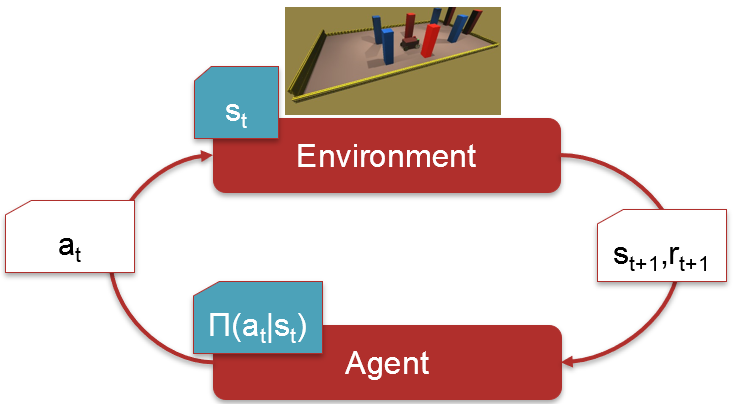
\includegraphics[width=0.8\textwidth]{Bilder/rl_cycle.png}
%    \caption{Loop in Collect Data}
%    \label{fig:unitycommunication}
%\end{figure} % TODO can we use this image?

Recent avancements in artificial intelligence technology have made it possible to develop automated solutons for a wide range of tasks that were previously thought to be too complex and unfit for machines to solve. Most notably over the last few years is the introduction of diffusion image models and large language models. These technologies were well recieved and moved artificial intelligence tools into public discourse. All over the world people have recognized the potential of artificial intelligence technologies and are now using them in their daily life and at work.

Artificial intelligence has already been of big importance in academia and industry for a long time. AI has been proved useful in many different fields, such as image recognition, natural language processing, and robotics. This encourages researchers and industry to further develop and use AI in their work. A promissing domain for the application of AI is autonomous driving.

The development of autonomous vehicles promises to greatly reduce the number of traffic accidents and transportation cost \autocite{mckinsey}. The development of autonomous driving could have further downstream effects on our society and industry, such as for example improved logistic and transportation systems.
As a result, researchers and private enterprises from all over the globe are making progress towards fully autonomous driving agents. Many companies started to integrate adaptive cruise control and lane centering assistance \autocite{carreviews} in their products. Due to the recent developments in artificial intelligence and the very high complexity of the task of autonomous driving, artificial intelligence often plays a big role in these systems \autocite{drl_for_ad}.

Predictions for the future of autonomous driving have been very optimistic and although huge progress has been made, the task of fully autonomous driving is still far from being solved \autocite{state_of_autonomous_driving2023}. This thesis aims at contributing to the research in this field by applying reinforcement learning to autonomous driving agents in a simulated environment. This work builds upon the work of \autocite{maximilian} and will use the same task and evaluation metrics. This thesis focusses on improving the agent's resiliency to changing light conditions by training a convolutional neural network end-to-end using reinforcement learning.


\chapter{Research Goals}
\label{cha:ResearchGoals}

The goal of this thesis is to contribute in the domain of autonomous driving by investigating the use of \ac{RL} to train an autonomous driving agent that is resilient to changes in light conditions. The agent is evaluated on simulated tracks that consist of a series of goals indicated by two blocks, a tracks is successfully completed if the agents drives through all goals in order \ref{fig:track_and_agent}.
This thesis builds upon previous work at the ScaDS.AI \textcite{maximilian} and uses the same tracks and task specifications. The agent from previous work was not able to reliably complete tracks under changing light conditions, motivating the research goals.


The agent and the policy are designed to be resilient to light changes. To achieve this, the policy is trained using \ac{RL} in a simulated environment with changing light conditions. The policy consists of a \ac{CNN}, the inputs to the \ac{CNN} are camera images from the perspective of the agent \ref{fig:track_and_agent}. Preprocessing steps are applied to the camera images to improve the performance of the policy under changing light conditions. The policy is trained end-to-end using an \ac{RL} algorithm. This allows the policy to learn the relevant features from the camera images itself.
Different training approaches and preprocessing steps to develop a powerful agent are investigated.


\begin{figure}
    \centering
    \subfigure{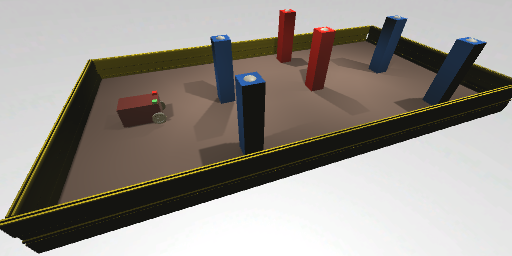
\includegraphics[width=0.4\textwidth]{Bilder/image_printer_images/evaluation_hard.png}}\qquad
    \subfigure{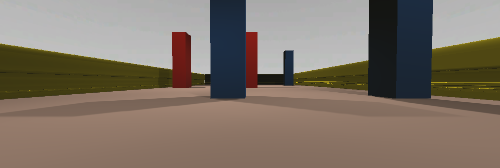
\includegraphics[width=0.4\textwidth]{Bilder/image_printer_images/agent_image_from_unity.png}}\\
    \caption{Example image of a track and the agent's camera}
    \label{fig:track_and_agent}
\end{figure}


\section{Question 1 - \questionOne}

The previous work by \textcite{maximilian} showed that it is possible to train an agent using \ac{RL} to solve the evaluation tracks, however the trained agents were not successful in reliably traversing the tracks of higher difficulty levels. The agents developed in previous work utilized an extensive preprocessing pipeline to extract the relevant information from the camera images for processing by the policy. The evaulation by \textcite{merlin_flach} showed that the preprocessing pipeline's performance depends heavily on the light settings of the environment.

This thesis will use a \ac{CNN} network policy that is trained end-to-end using \ac{RL}. It has already been shown to be possible to train an agent to solve the autnomous driving task using \ac{RL}. However the agents developed in previous work used different preprocessing steps and policies compared to the agents developed here.

Due to these differences in implementation and as a prerequisite for question 2 and 3, it is first important to investigate if it is possible to train a \ac{CNN} policy to reliably solve the tracks of all difficulty levels. This raises question 1:
\questionOne

The question will be answered by developing agents based on related work. The training process of the agents will use common practices from \ac{RL} adapted to the specific task. The developed agent's $success\_rate$ and $collision\_rate$ will be evaluated on all difficulty settings to answer the question.


\section{Question 2 - \questionTwo}

Question 1 investigates if it is possible to develop a successful \ac{CNN}-based agent solving the tracks of all difficulty levels. 
Question 2 then investigates if it is possible to make the \ac{CNN}-based agents robust to changing light conditions.

The agents developed for question 1 will be used as a basis for the agents developed in this question. The agents will be augmented with preprocessing steps that improve the performance of the agents under changing light conditions. These preprocessing steps will be applied to the camera images before they are processed by the policy. The agent's policy will be trained in a simulated environment with changing light conditions to help the agent generalize and learn.

Similarly the $success\_rate$ and $collision\_rate$ will be primarily used to evaluate and compare the agent's performance. The performance difference between different light conditions will be used to answer the question. If the performance for all light conditions is comparable to the performance of agents in question 1, the agents can be considered robust to changing light conditions.

\section{Question 3 - \questionThree}

One goal of the ongoing research at the ScaDS.AI is to build physical robots for demonstration and research purposes \textcite{merlin_flach}. The robots are based on the NVIDIA JetBot platform \autocite{jetbot}. They are equiped with a camera, wheels and a small on-board computer. A future goal is to transfer trained policies onto these robots and execute them in real-life. However the limited processing power of these robots might not be sufficient for more complex agents that utilize \acp{NN}. This raises question 3 - \questionThree


The question will be answered by investigating the processing power required to run the preprocessing steps and \acp{NN} used in the agents. This will be evaluated empirically by creating recordings of the agents in simulations. The recordings are then replayed on the physical hardware. The evaluation checks if the physical hardware is able to reproduce the preprocessing steps and policy from the replays in real-time.



\chapter{Related Work}
\label{cha:Related Work}


The development of self-driving cars represents one of the most intricate and ambitious challenges in the field of engineering, robotics and artificial intelligence. The complexity and variability of real-world driving environments make this task extremely difficult. The environments include unpredictable actors, such as other drivers, pedestrians, and animals, as well as changing weather and road conditions. The environments include uncounted edge cases that are difficult to anticipate and code for explicitly. Consequently, many researchers and institutions include advanced machine learning techniques in their approaches towards solving autonomous driving.

The development of autonomous driving systems started with driver assistance systems in the 1970s. These systems focus on assisting the driver in specific tasks, such as lane keeping, adaptive cruise control, and parking. This reduces the problem complexity. However modern self-driving systems aim to achieve full autonomy. For example the Tesla autopilot is capable of driving in many environments without human intervention.

This thesis will use reinforcement learning in the training of an autonomous driving agent. The agent is equiped with a single camera sensor. The agent's behaviour is controlled by a convolutional neural network that processes the visual input. The agent has to learn a specific self driving task with reduced complexity. The self-driving task is similar to previous research at the ScaDS.AI \textcite{maximilian}. However the agent design and training is very different.
The task consists of a restricted environment. The environment consists of an enclosed arena with different tracks that the agent has to complete. The tracks consist of a series of goals that the agent has to drive through. The tracks are grouped in three difficulty levels.
The environment is simulated with three light settings. The trained agent has to learn to navigate all difficulty levels and light settings.

Research relating to reinforcement learning algorithms, convolutional neural networks and self-driving will be reviewed.
% also research regarding rebustness to light changes?

% TODO auch die Ergebnisse der Paper und die daraus gezogenenn Schlüsselideen erwähnen


\section{Self-Driving}

Neural networks have been used in the domain of self driving for a long time. Pomerleau \textcite{alvinn} developed one for the first self driving systems with neural networks in 1989. The system was developed for road following. The system used a camera image and a laser range finder as input. Compared to current network sizes, they used a small fully connected neural network. The network was trained using synthetic data. The data consisted of generated road images and steering commands. The network was trained using backpropagation to reproduce the steering commands. This approach did not use reinforcement learning. The system was able to follow roads in real-life under certain conditions.
The paper highlights the advantages of neural networks for self-driving. The training data determines the salient image features and not the programmer. This has proven to be true with the success of convolutional neural networks in the domain of self-driving \textcite{neptune}.


There has been a lot of progress in the domain of self-driving in recent years. Sophisticated self-driving algorithms consist of many hardware and software components to achieve satisfying performance. Hardware components include various imaging approches such as Radar, Lidar and cameras. Termometers and other hardware components are also used, for example to determine weather conditions. 
Software components might include separate object detection, occupancy and planning. For example Tesla's self-driving builds these components on top of a shared backbone that uses convolutional neural networks \textcite{howteslaautopilot}.
% (CNN is ResNet)

Self-driving in a real world environment is a very complex task, especially when including other traffic participants. Modern self driving agents consist of multiple complex components that interact with each other \textcite{drl_for_ad}. Components for Scene Understanding build a model of the current surroundings. The Descision making \& Planning components use this model to decide and execute the next actions.
Multiple interacting components are shown in figure \ref{fig:ad_components}.

\begin{figure}
    \centering
    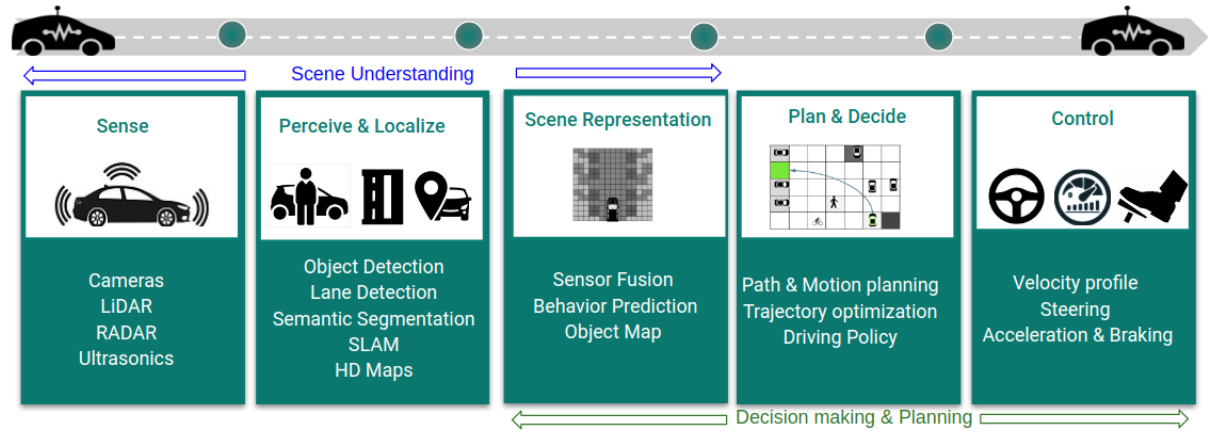
\includegraphics[width=0.8\textwidth]{Bilder/ad_components_from_paper_drl_for_ad.png}
    \caption{Standard components in a modern autonomous driving systems pipeline listing the various tasks. The key problems addressed by these modules are Scene Understanding, Decision and Planning. Image from \textcite{drl_for_ad}}
    \label{fig:ad_components}
\end{figure}

An agent with similarly complex components is not feasible for this thesis. The agent in this thesis uses a single convolutional neural network to process the visual input and make decisions instead. I aim to contribute to the domain by expanding on previous research and focus on the training of a convolutional neural network agent. 


TODO wohin diesen satz?
Approaches from the domain of self-driving will be used to improve the training of the agent, for example reward shaping \textcite{drl_for_ad}.

\subsection{Previous Work}
This thesis builds directly upon the work of Knig \textcite{jonas_koenig}, Flach \textcite{merlin_flach} and Schaller \textcite{maximilian}. 
\textcite{jonas_koenig} built a self-driving agent that was trained to avoid collisions in a simulated arena. The agent used a hand-crafted preprocessing pipeline to extract features from visual input. The features represent the obstacles that the agent has to avoid. The agent's behaviour was controlled by a policy that consisted of a neural network. This network used the extracted features as inputs. It was trained using an evolutionary approach in simulation.

\textcite{merlin_flach} investigated the feasibility of transferring this agent to the real world. The research showcased many challenges. The challenges are caused by differences between the simulated and real-life environments, the Simulation-To-Reality gap. The most notable problem was the object recognition part. The preprocessing pipeline had difficulties recognizing the objects in the real world. This results in further problems for the agent, since the agent's policy is based on the extracted features.

\textcite{maximilian} investigated a different task than the two previous papers. An agent was trained to traverse a track by driving through a sequence of goals. The same tracks are used in this paper. The agent used a preprocessing pipeline to extract object features similar to \textcite{jonas_koenig}. The neural network policy was trained using the proximal policy optimization \textcite{ppo} reinforcement learning algorithm. The agent could traverse the tracks, its performance decreased for tracks of higher difficulty. Further evaluation of the agent under different light settings showed that the agent is not robust to changing light conditions. The preprocessing pipeline was not able to extract the necessary features reliably under different light settings, this resulted in a performance collapse.

The instability of the hand-crafted preprocessing pipeline and promissing results by CNNs from other RL researchers in the domain of self-driving \textcite{neptune} motivate the choice of CNNs as the feature extraction method in this thesis. 


\section{Reinforcement Learning}

% data not programmer decides the salient image pixels (bedeutungsvollen)
\subsection{Introduction to Reinforcement Learning}

Reinforcement Learning algorithms have been around for a long time, but only recently have they been able to achieve superhuman performance in games and control tasks \textcite{atari}. Reinforcement learning algorithms formalize the problem as consisting of an environment and a policy $\pi$. The environment consists of a state space, an action space and a reward function that takes state-action pairs as input. Reward functions assign positive rewards to actions that are deemed to be desirable by the environment designers, for example scoring a goal in a football match. Reward function can also assign negative rewards to undesirable actions, for example collisions in a driving simulation. 

The goal of reinforcement learning algorithms is to build an agent that interacts with its environment and maximizes the cumulative reward over time. The policy selects actions given an observation. It controls the agents behaviour \textcite{rlbook2020}. It is trained by the \acs{RL} algorithm to learn the desired behaviour. The trained policy can then be used to solve problems in the environment. 

The agent interacts with the environment during the training phase of RL algorithms. The policy takes some representation of the environment's state as input and selects actions to execute in the environment. The selected actions are executed in the environment by the agent which results in a new state. The reward function assigns rewards to these state transitions.
The observed rewards are then used to update the policy \ref{fig:rlcycle}.

\begin{figure}
    \centering
    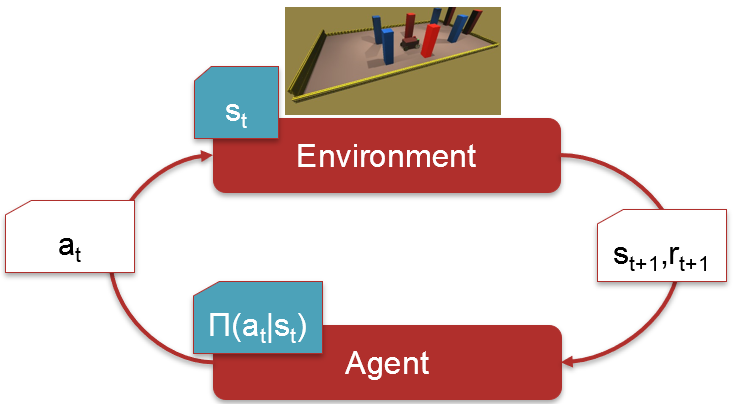
\includegraphics[width=0.4\textwidth]{Bilder/rl_cycle.png}
    \caption{RL Training Cycle: The agent selects action $a_t$ based on policy $\pi(a_t|s_t)$ at state $s_t$ and recieves the next state $s_{t+1}$ and rewards $r_{t+1}$ from the environment. The states, actions and observed rewards are used to update the policy.}
    \label{fig:rlcycle}
\end{figure}

\subsection{Classification of \acs{RL} Algorithms}

Reinforcement learning algorithms are classified into two major groups. RL algorithms that use a model of the environment are called model-based algorithms, algorithms without such models are called model-free algorithms. Algorithms from both groups have been successfully used in a wide range of applications, model-based algorithms are often much more complex but have been shown to be successful at many task that require planning \textcite{alphagoimprovementmuzero}. Model-free approaches are often simpler and more flexible, they have shown great success in various control tasks \textcite{atari}.

\begin{figure}
    \centering
    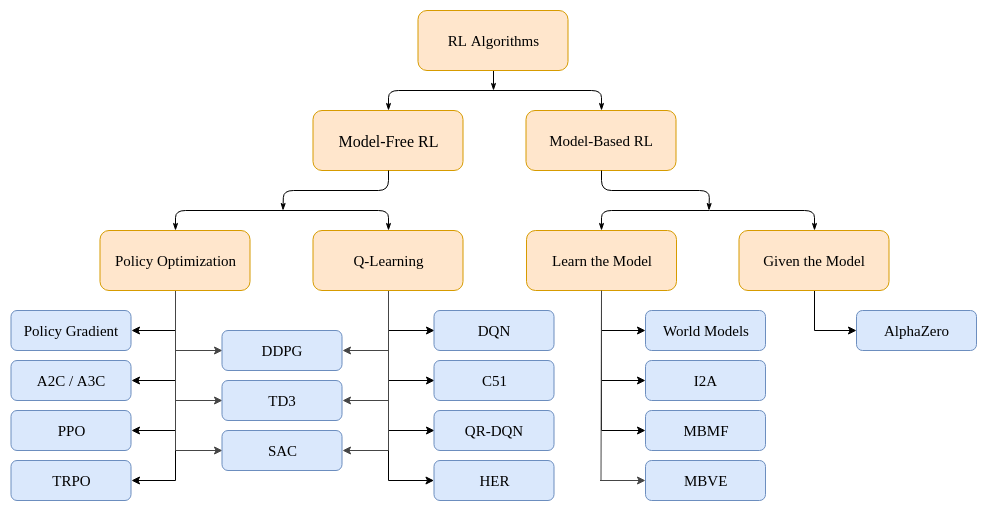
\includegraphics[width=0.8\textwidth]{Bilder/openai_spinningup_taxonomy.png}
    \caption{Taxonomy of RL algorithms from OpenAI's Spinning Up course \autocite{spinningup}}
\end{figure}

\subsubsection{Model free \acs{RL} Algorithms}

\paragraph{Value based algorithms}
Model free algorithms can be further divided into two families. The first family are value-based approaches. These algorithms learn a function that assigns state-action pairs a value. This function is called the value function. This value represents the expected future reward Q.
 
The policy is not trained directly. The policy selects actions based on this value function instead. The state-action pair with the highest Q-value is selected for a given state.

The training process of the value function is done by updating the Q-values based on the observed rewards. The Q-learning algorithm is an early and common example of value-based algorithms \textcite{rlbook2020}. The Q-learning algorithm updates the values based on the observed rewards and the maximum Q-value of the next state \[Q(S_t, A_t) = Q(S_t, A_t) + \alpha (R_{t+1} + \gamma \max_a Q(S_{t+1}, a) - Q(S_t, A_t))\].
$\alpha$ is the learning rate. It determines how quick values are changed. $\gamma$ is the discount factor of future rewards.


The Q-learning algorithm can use a table to store the value function. The table contains one cell for each state-action pair and stores the Q-value. 
For many problems the use of these tables in not feasible due to the amount of state-action pairs, many extensions to the algorithms have been developed such as for example deep q-learning. Deep q-learning uses a deep neural network to approximate the Q-values \textcite{atari}. The network learns to predict the Q-values for state-action pairs. Neural networks are general approximators. They can learn to generalize and return accurate value predictions even for previously unseen states.  

Value-based \acs{RL} algorithms have been used to great success for control tasks \textcite{rlbook2020}. However they will not be used in this thesis, as they require discrete action spaces. The environment in this thesis consists of a continuous action space.
An action space can be discretized for use by value-based algorithms \ref{fig:example_discretization}. However this can lead to a loss of fidelity.

% TODO \ref{fig:example_discretization} ?

\paragraph{Policy based algorithms}
% rlbook2020 chapter 13.7
The other family are policy-based algorithms. These algorithms optimize the policy directly instead of the values associated with states or state-action pairs. Instead of computing the learned probability of each action, the policy learns the statistics of the action distribution.
Given a scalar action space. The action distribution can be represented as a gaussian probability Distribution:
\[p(x) = \frac{1}{\sqrt{2\pi\sigma^2}} e^{-\frac{(x-\mu)^2}{2\sigma^2}}\]

The policy can then be defined as the normal probability density over a real-valued scalar action. The mean and standard deviation of the distribution are given by parametric function approximators that depend on the state $s$. The mean is given by $\mu(s, \theta)$ and the standard deviation by $\sigma(s, \theta)$. The policy is then defined as:
\[\pi(a|s, \theta) = \frac{1}{\sigma(s, \theta)\sqrt{2\pi}} e^{-\frac{(a-\mu(s, \theta))^2}{2\sigma(s,\theta)^2}}\]

The parametric function approximators $\mu(s, \theta)$ and $\sigma(s, \theta)$ are trained by the \acs{RL} algorithm. Any function approximator can be used, for example a \acs{NN} with parameters $\mu$ \textcite{rlbook2020}. 

The action distribution can be extended to multi-dimensional action spaces. This action distribution can be represented as a multivariate gaussian distribution. The function approximator then outputs the mean and covariance matrix of the distribution. This makes policy-based \acs{RL} algorithms very flexible. They can be used for multi-dimensional continuous action spaces.


The policy can be updated using the gradient of the expected rewards with respect to the policy parameters. Algorithms that use this approach are called policy gradient algorithms.


\paragraph{Actor-Critic Algorithms}
Alternatively the policy can be updated using Actor-Critic approaches. These combine policy-based and value-based approaches. Actor-Critic approaches contain a policy and a value function. The value function represents the expected future reward of a state. The policy is updated using this value function.

The Proximal Policy Optimization algorithm is an Actor-Critic algorithm. It was developed to improve the stability of policy-based algorithms \textcite{ppo}. The \acs{PPO} algorithm restricts the size of policy changes caused by parameter updates, which ensures the policy does not change drastically. This improves stability. \acs{PPO} is currently one of the most popular algorithms for reinforcement learning. It has already been successfully used in the domain of autonomous driving \textcite{maximilian}.



% Another major improvement in the domain of reinforcement learning was the combination of neural networks with traditional planning and search algorithms, the most famous example for this is AlphaGo \textcite{alphago}. These algorithms often are model-based algorithms and use search algorithms (e.g. Monte Carlo Tree Search)  to evaluate the possible actions at a given state. The neural networks are used for the evaluation of states and actions in the search algorithms. AlphaGo was developed for a 2 player deterministic game with a discrete state and action space. Since then this combination of neural networks and search algorithms has also been used to achieve impressive results for all kinds of problems \textcite{alphafold}, for example single player continuous state and action spaces \textcite{alphagoimprovementmuzero}. Although these algorithms could be applied to the problem at hand, they will not be utilized due to the increased complexity of the algorithms and the required computational resources.
% TODO sollte der Teil wieder rein?

% temporal difference learnign: update a function based on previously learned things (e.g. q-learning)

% TODO mention reward shaping from rlbook somewhere
% first give a reward signal that is not aligned with final goal but gives frequent rewards
% train the agent using this function
% change function over time to the intended reward function (event Reward)
% learning behaviour is guided by the shaped reward function



\subsection*{Convolutional Neural Network for Reinforcement Learning}

Convolutional neural networks are a neural network architecture specifically developed for processing image data, they consist of a number of filters and a fully connected neural network. The filters are applied to the image in a sliding window fashion, the filters detect patterns in the image such as for example edges and corners. Multiple successive applications of such filters enables the network to learn hierarchical information and recognize more complex structures. The fully connected neural network analyses the results of the filters and makes the final prediction \textcite{rlbook2020}.

CNNs are often used in Reinforcement Learning since RL problems often require an agent to process visual input. Furthermore CNNs can be trained end-to-end in Reinforcement Learning compared to other feature extraction methods, which means the CNN can learn what features are important for the task at hand.
Therefore a convolutional neural network will be used to process the camera images instead of a hand-crafted feature extraction method. 

CNNs typically do not take the raw camera/simulation images but rather preprocessed images, e.g. greyscaled images \textcite{atari}. Preprocessing steps can help in reducing the complexity of the input space. Convolutional neural networks require a lot of data to train, data augmentation can help increase the size of the training set and to make the agent more robust. Data augmentation generates new samples from already collected ones by applying transformations to the samples. 


% TODO move next paragraph to CNN section?
The PPO algorithm can be used to train agents that use convolutional neural networks as their policy. Convolutional neural networks are ideal for processing image data and can be trained end-to-end by the algorithm \textcite{ppo}. 

% rlbook2020 chapter 9.7 explains the use of CNNs in RL



% \textcite{autonomous_vehicles_review} %TODO read this paper and cite it

% https://safe-intelligence.fraunhofer.de/en/autonomous-driving

% Papers that use Carla



\section{Simulation for Reinforcement Learning and Self-Driving}

% TODO Carla und andere Simulations machen keinen Sinn, da wir ein festse Problem haben

Simulations play a huge role in reinforcement learning and thus the development of self-driving agents. Simulations provide a huge number of benefits over real world experiments. They are much cheaper and faster to run than real world experiments, furthermore they can be run in parallel. In addition the programmers have direct and perfect control over the environment, as such programmers can for example change the simulation speed. This allows for fast experimentation and training of reinforcement learning agents. Simulations also allow for the creation of scenarios that are not possible in the real world. This is especially useful for reinforcement learning agents that are trained to avoid collisions. Simulations also allow for the creation of ground truths such as perfect sensor data and object bounding boxes \textcite{carla}.

Simulated environments often serve as baselines for reinforcement learning algorithms, most famous are the atari games \textcite{atari}. The Python Gynasium API was developed for easy reuse and comparison of reinforcement learning algorithms for different problems \textcite{gymnasium}, the Gymnasium API defines an interface that can be used to model tasks as reinforcement learning problems. A wide range of reinforcement learning frameworks support the Gymnasium API, for example Google's dopamine \textcite{dopamine} and OpenAI's baselines \textcite{sb3}. Advanced simulations like the Unity engine \textcite{unity}, the physics simulator MuJoCo \textcite{mujoco} and the driving simulator Carla \textcite{carla} can be integrated with the Gymnasium API.

%The complexity and interest in self-driving has also led to the development of dedicated simulators, such as the Carla \textcite{carla} and the AirSim \textcite{airsim} simulator. The Carla simulator provides researchers with useful features such as weather control and ground truths for object detection and segmentation.

There are also dedicated frameworks for reinforcement learning that directly integrate with simulation engines. \textcite{maximilian} used the ML-Agents framework \textcite{mlagents} to train the self-driving agent in Unity directly.

In this thesis Unity will be used for the simulation, the simulation will be integrated with the Python Gymnasium API and PPO algorithm. This approach is chosen instead of the ML-Agents framework since it allows for more flexibility and control over the simulation and training process.


\section{Imitation learning}
As described before it is difficult to build self-driving agents for real world environments due to the environment complexity. The amount of complex edge cases make it very difficult to programmatically define the agent's behaviour. Neural networks can be used to control the agent behaviour instead. The neural networks can be trained using reinforcement learning in simulation. 
Imitation learning is another approach to training an agent that interacts with its environment. Imitation learning requires a dataset that demonstrates the desired behaviour. The agent is trained on the dataset to mimic the expert behaviour.

In reinforcement learning the programmer has to define a reward function that the agent uses to learn and improve its behaviour. In imitation learning the agent learns exclusively from the dataset. As a result this dataset has to include a wide range of scenarios to produce a reliable agent that can handle edge cases.

There are two approaches to training an agent with imitation learning, behavioural cloning and inverse reinforcement learning. Behavioural cloning is the simpler approach, the agent learns to mimic the expert behaviour directly. This is similar to supervised learning. Inverse reinforcement learning is more complex, the reward function from the expert demonstrations is learned first. The agent is then trained to maximize this reward function using reinforcement learning. 

Bojarski \textcite{bojarski2016endToEnd} used imitation learning to train a self-driving lane following agent for real-world environments. This agent consists of a convolutional neural network that processes the camera images and predicts the steering angle directly. The agent is trained end-to-end to reproduce steering behaviour from recorded data. They demonstrate that imitation learning is a viable approach for developing an agent without the need for multiple components such as object detection and path planning.

Tesla used imitation learning to train the path prediction component of their self-driving systems. The fleet of Tesla vehicles allows them to collect a large amount of representative data in the real world. The reference dataset was generated from recordings of human Tesla drivers \textcite{tesla_youtube}. 

Imitation learning and reinforcement learning can be combined to improve the training of the agent. The reinforcement learning process generates samples via interaction between agent and environment. These samples and the expert behaviour dataset are used together to train the agent policy \textcite{car-following_carla_dresden}.


%\section{Reinforcement Learning for Self-Driving}

%\textcite{drl_for_ad} review the use of reinforcement learning for autonomous driving, they also describe many improvements for reinforcement learning algorithms that can improve the training stability and performance, such as for example reward shaping.
%In addition to published research papers there have been a lot of experiments, tutorials and demonstrations of self-driving agents on YouTube and GitHub. The University of Tübingen published their full lecture series on Self-Driving Cars \textcite{tuebingen}, the series also includes a section on reinforcement learning.

% papers that cite carla: https://scholar.google.de/scholar?cites=660591080772510291&as_sdt=2005&sciodt=0,5&hl=de


% Tübingen: % https://www.youtube.com/watch?v=GYnlqiSqZiU&list=PL05umP7R6ij321zzKXK6XCQXAaaYjQbzr&index=13



% Key Papers in RL: https://spinningup.openai.com

\section{Light change resiliency}

\subsection{Domain Randomization}

useful for transfer sim-to-real
https://ar5iv.labs.arxiv.org/html/1703.06907

domain randomization for sim-to-real tries to teach the agent to solve a task under a big variety of conditions in simulation, the hope is that the agent will be able to generalize this variation and learn in this environment.
The real world is simply one variety that the agent might have already learned to generalize.

The randomization can include textures, image resolutions, ..., motor power of agent in sim, ... (physical properties)


domain randomization can lead to a high variance of policy performance for different environment randomizations. The paper https://ar5iv.labs.arxiv.org/html/1910.10537 introduces a regularization approach for the policies.
visual vs dynamics randomization (camera changes vs physics e.g. friction of wheels)

\subsection{Data augmentation}

Data is collected in simulation and then augmented


\subsection{Multi-Modal learning}

Provide the agent with more than just image data,  e.g. radar...


\subsection{Hierarchical Reinforcement Learning}

combination of multiple levels. higher level policy controlls the actions, the lower level policy learns to build representations for the higher level policy

Hierarchical Reinforcement Learning: Using a hierarchical approach where high-level policies govern low-level policies can help the agent adapt to changing conditions more effectively. High-level policies can decide on strategies based on the overall environment, while low-level policies handle specific tasks like adjusting to lighting changes


TODO relate the previous work that used a hand-crafted feature extraction pipeline to hierarchical rl

\section{Transfer to reality}

\subsection{Transfer Learning}
learn on diverse data and then fine-tune on real data


\section{Key Ideas}

\subsection{Fitting RL algorithms}

\subsubsection{CNN for feature extraction in RL}

\subsubsection{Memory mechanism}


\subsection{Reward shaping}

\subsection{Environment Implementation}

speed of environment is critical...


\subsection{Image preprocessing for resiliency to light changes}

\subsection{Domain Randomization}






\chapter{Methods}
\label{cha:Methods}



\section{Task Description}

In this section I will be describing the task and the simulation environment as these two aspects are the foundation of this thesis and will not change over the course of the project.
The task is to develop an agent using reinforcement learning that is able to complete a parcour in a simulated environment without collisions. The agent has to traverse the parcour by passing through a number of goals indicated by pairs of either red or blue blocks without collisions. This problem belongs to the class of single player continuous state and action space problems. At each timestep the agent uses a neural network to process an image from the environment and produce two actions. The two actions are the acceleration values of the left and right wheel, these acceleration values are applied to the wheels until a new action is selected.% The timesteps do not have a fixed duration, a new timestep is started as soon as the last one is finished. The amount of timesteps per minute will be measured? This is like FPS?

The task and agent are simulated using the Unity game engine, the game engine handles the rendering of the environment, collisions, agent movement and reward functions.


\begin{figure}
     \centering
     \subfigure[Example image of the agent at the start of a parcour with 3 goals in Unity]{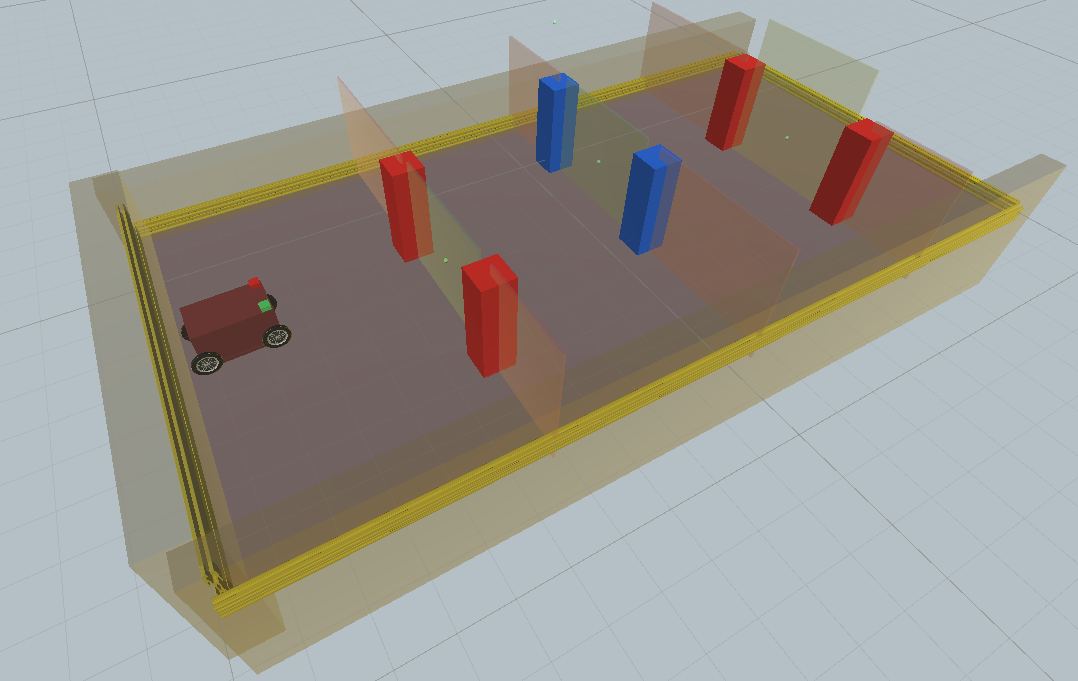
\includegraphics[height=5cm]{Bilder/parcour.png}}\qquad
     \subfigure[Agent camera view]{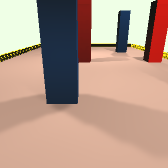
\includegraphics{Bilder/agent_input_image2.png}}\\
     \caption{Unity simulation environment and agent camera view}
\end{figure}


\iffalse
     \begin{figure}[h!]
          \centering
          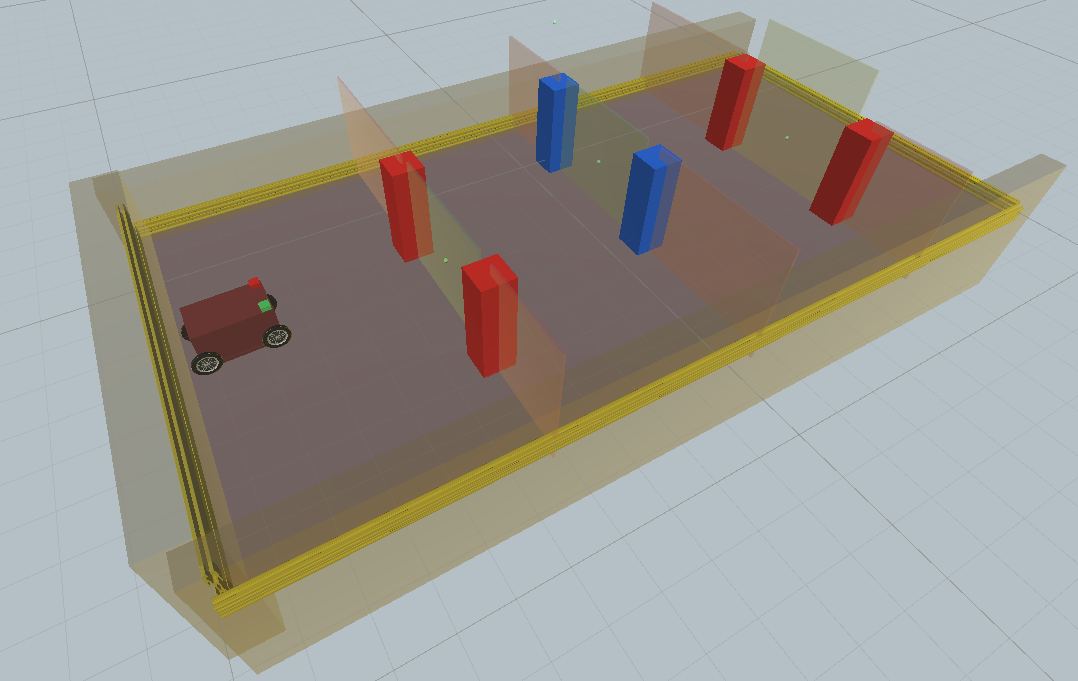
\includegraphics[height=7cm]{Bilder/parcour.png}\\[2.5ex]
          \caption{Example image of the agent at the start of a parcour with 3 goals in Unity}
          \label{task}
     \end{figure}
     \begin{figure}[h!]
          \centering
          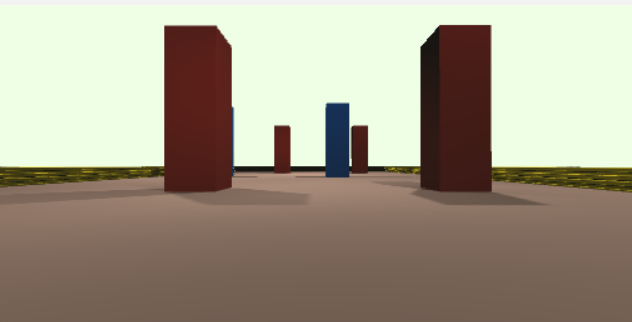
\includegraphics[height=7cm]{Bilder/agent_input_image.png}\\[2.5ex]
          \caption{Example image that will be processed by the agent's convolution neural network.}
          \label{input_image}
     \end{figure}
\fi

% mention the similarity/simplicity of the task


\section{Reinforcement learning algorithm and frameworks}

As outlined in the related works section many different RL algorithms can be used to solve single player continuous state and action space problems. The PPO algorithms is most commonly used for problems of this class and has already been successfully used in the investigated task \autocite{maximilian}. The MuZero \autocite{alphagoimprovementmuzero} could also be used, however this algorithm does require a lot more compute resources during training and inference.
In this thesis the PPO algorithm will be used.

There are multiple approaches to training an agent in the Unity simulation environment as highlighted in the related works section, it is not yet decided which approach will be chosen, therefore I will quickly describe the possible scenarios and highlight their advantages and disavdantages.

\subsection*{Unity and ML-Agents}

Reinforcement learning agents can be trained directly in the Unity simulation environment using the ML-Agents framework \autocite{mlagents}. This approach has the advantage of being very simple to implement and use, since the agent and simulation are in the same framework. The biggest disadvantage of this approach is that it might be difficult to implement some of the implementation details that might be used in this thesis such as the proposed changes for dealing with delayed rewards.
The PPO algorithm by \autocite{mlagents} was used in \autocite{maximilian} to successfully train the agent on the investigated task.

\subsection*{Unity and separate reinforcement learning frameworks}

There are many reinforcement learning frameworks publicly available that can be used to train agents in simulated environments, such as the OpenAI's baselines \autocite{sb3} and Google's dopamine \autocite{dopamine}. These frameworks often support the Gymnasium API \autocite{gymnasium}, wrapping the Unity simulation environment in a Gymnasium environment would allow for easy use of these frameworks. This approach has the advantage of being able to use the many features of these frameworks and makes it easy to change the training algorithms which might be necessary for the investigated implementation details. The disadvantage of this approach is that it might be difficult to wrap the Unity simulation environment in a Gymnasium environment, there already exist frameworks to help with this \autocite{peacefulpie}.


% maybe mention the similarity/simplicity of the task here to show PPO is good


\section{Investigated implementation details}

The goal of this thesis is to answer two questions with a subitem each.
\begin{enumerate}
     \item Is it possible to train an agent to reliably solve the parcours of all difficulty levels?
           \begin{itemize}
                \item Are memory mechanisms necessary in achieving this?
           \end{itemize}
     \item Is it possible to use an end-to-end trained CNN to make the agent robust to changing light conditions?
           \begin{itemize}
                \item Is it possible to use a CNN which is small enough to be used in the JetBot?
           \end{itemize}
\end{enumerate}

\subsection{Improvements for training the agent}

\subsubsection{Reward shaping}

Reward shaping is the practise of providing reinforcement learning agents with frequent and accurate rewards. This helps the agent develop the desired behaviour quicker and more reliably since reward signals are less sparse with reward shaping \autocite{drl_for_ad}. This practice was already employed by \autocite{maximilian} by providing the agent with a reward proportional to its speed, this encourages the agent to drive faster and thus hopefully complete the parcour quicker. This thesis will investigate the use of a reward proportional to the difference in distance to the next goal between timesteps, this should encourage the agent to drive towards the next goal and to drive faster in this direction.


\subsubsection{Dealing with delayed rewards}
Delayed rewards can be a big problem in reinforcement learning and make the training process difficult. Delayed rewards are rewards that are not obtained immediately after the responsible action is taken. In our environment an action \(a_n\) (e.g. turning right) may lead to a collision at state \(s_{n+x}\) which results in a negative reward for action \(a_{n+x}\). The RL algorithm might fail learn to avoid the action \(a_n\).

There are a multiple approaches to dealing with delayed rewards. These approaches use the reward at the current timestep and the near future. These approaches result in a more accurate and dense reward signal and can improve the training stability and performance of the agent.
N-step bootstrapping uses the rewards at the current step and the next \(n\) steps \autocite{nstepbootstrapping}.
A similar approach does not use the reward from the next \(n\) steps but rather the cumulative reward encountered in the next \(n\) seconds \autocite{trackmania}. Due to the continuous nature of the environment this approach might be more suitable than the previous one.


\subsubsection{Time perception}

Two configurations of the agent by \autocite{maximilian} used a memory to enhance the agent's input, the memory consisted of the input of the last few steps of the agent. This technique of stacking the history has been widely used in RL for continuous \autocite{atari} and discrete action spaces \autocite{alphago}. This allows the agent to perceive object movement, time and velocities \autocite{atari}.
In our case the agent needs a history since the next goal could leave the agent's current field of vision.

%However since the investigated environment does not have fixed timesteps this approach might not be as effective. The time elapsed between two steps can vary due to many factors such as varying compute resources. It could prove useful to provide the model with the input of the last few steps and in addition the elapsed time between these steps. % these few sentences only make sense if the varying time is dicussed in the first part of the Methods section

% TODO test other memory mechanisms?
% like for example also feeding the previous time step's hidden layer activation as input
% that way the agent would know the previous "decision" not just the previous input

\subsection{Improvements for Light setting robustness} \label{light_setting_robustness}

\subsubsection{Convolutional Neural Networks}

The works by \autocite{merlin_flach} and \autocite{maximilian} showed that the agent's performance greatly depended on the quality of the input preprocessing pipeline. This object detection pipeline had difficulties detecting objects under varying light settings. This thesis will investigate using convolutional neural networks instead of an object detection pipeline, this should make the agent more robust to varying light settings and improve the performance of the agent.
Using convolutional networks to process images is a common practise in the field of reinforcement learning, due to the ability of these networks to adapt. The convolutional neural network could potentially learn to identify relevant information in images more reliably than the previously used image detection pipeline. The research by \autocite{merlin_flach} showed that not all the information provided by the object detection pipeline was considered to be relevant by the neural network, this could be mitigated by training the CNN end-to-end.
As a starting point for experimentation the CNN architecture will be the same as \autocite{human_level_control}.

% we use the default CnnPolicy network, is it the same as the one described in Atari?
% architecture: https://github.com/DLR-RM/stable-baselines3/blob/d671402c9373391f44d8a2ad11deed615e0f4bae/stable_baselines3/common/torch_layers.py#L89-L106
% it is exactly as described in "Human-level control through deep reinforcement learning"
% \autocite{atari} has a slightly smaller NN

% (more robustness?) (previous input was shit (sim2real paper wegen x, y, width, height input problem)) (previous system higly depended on bounding box detection)


\subsubsection{Feature reduction / preprocessing}

There are several preprocessing approaches that can be used to prepare an image for processing by a convolutional network. The goal of these approaches is to reduce the feature space to increase processing speed, they can also help encourage the network to generalize. The following steps were taken in the foundational \autocite{atari} paper. These techniques will be used due to the similar complexity of our task and many atari games.

\begin{description}
     \item[Downsampling] reduces size of input space
     \item[converting to greyscale] reduces size of input space and potentially removes irrelevant information
     \item[Rescaling pixel values to between 0 and 1] can help the neural network learn quicker % see https://machinelearningmastery.com/how-to-improve-neural-network-stability-and-modeling-performance-with-data-scaling/
\end{description}


\subsubsection{Histogram Equalization}

The previous work this thesis builds upon used the HSV colour space to extract the differently coloured objects. colours in this space consist of three values, one for the hue, saturation and brightness. The hue value was used for extracting the objects. In theory the utilization of this colour space should make the object detection resilient to changes in brightness since this information does not affect the hue value.
Convolutional neural network typically use the RGB colour space or a greyscale colour space. A histogram equalization of the input images could play a big role in making the agent more resilient to changes in illumination, with which the agent by \autocite{maximilian} struggled with. Image d) in \ref{fig:4bildchen} shows the effect of histogram equalization on an image, the image looks worse for identifying objects. This suggests the equalization might not be necessary/useful, it is to be investigated during the implementation/experimentation phase.


%* histogram equalization / enhance contrast (preprocessing) https://stackoverflow.com/questions/39308030/how-do-i-increase-the-contrast-of-an-image-in-python-opencv

% \autocite*{drl_for_ad} shows a lot of best practises in RL for autonomous driving

\begin{figure}
     \centering
     \subfigure[Original Image]{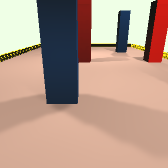
\includegraphics{Bilder/agent_input_image2.png}}\qquad
     \subfigure[Downsampled image]{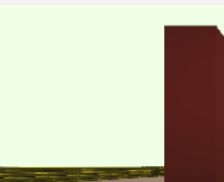
\includegraphics{Bilder/downsampled.png}}\\
     \subfigure[greyscale]{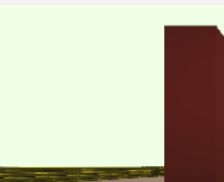
\includegraphics{Bilder/greyscaled.png}}\qquad
     \subfigure[histogram equalized image]{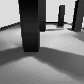
\includegraphics{Bilder/equalized.png}}
     \caption{4 Stages of preprocessing images for the CNN}
     \label{fig:4bildchen}
\end{figure}


\section{Training Process}


\subsection*{Training Parcours}
The PPO Reinforcement Learning algorithm requires the agent to be placed in a simulation environment similar to the evaluation environment to achieve good results. The agent will be placed in an arena with goal objects during training. In previous work \autocite{maximilian} two different training regimes were used, Single-Goal-Training and Full-Map-Training. In Single-Goal-Training the training was stopped after completing the first goal or upon collision. In Full-Map-Training the training was stopped after completing the whole map or upon collision. The reasoning behind Single-Goal-Training is that the agent will encounter a bigger variety of states during training since it will start at different positions in the map. However the Full-Map-Training scenario is closer to the evaluation scenario since the agent has to complete multiple goals in succession during evaluation.
Single-Goal-Training performed worse than Full-Map-Training in the previous work \autocite{maximilian} for all evaluation parcours except for the difficult one.

A third possible regime would be Full-Map-Training with randomized starting positions, this combines both approaches. The Single-Goal-Training is not strictly worse or better than Full-Map-Training. Therefore is not clear what training regime to chose for this thesis, therefore SGT, FMT and FMT with randomized starting positions will be compared during the experimentation phase.
% randomized starting positions also means start at random goals

\subsection*{Training Light Settings}
Since the agent utilizes a Convolutional Neural Network to be resilient towards changing light conditions it is also necessary to train the agent with varying light conditions, otherwise the adaptability of the CNN would not be fully utilized. This way the agent will be able to learn to generalize to different light conditions. The light conditions will be randomized for each training parcour.
Training with fixed light settings could also provide interesting insights when comparing the results to the results of training with varying light settings. If there is enough time the agent will be trained with fixed light settings as well. The comparison would show if the varying light settings during training helps for the generalization to different light settings.

% TODO put a figure with randomized light settings here
% maybe camera image from agents with different light settings

\begin{figure}
     \centering
     \subfigure[standard lighting]{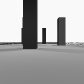
\includegraphics{Bilder/light_setting_standard.png}}\\
     \subfigure[reduced lighting]{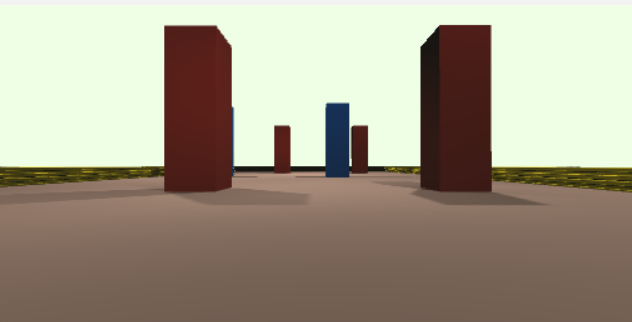
\includegraphics{Bilder/light_setting_reduced_lighting.png}}
     \subfigure[Increased lighting]{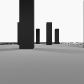
\includegraphics{Bilder/light_setting_increased_lighting.png}}
     \caption{different lightings TODO fix the images}
     \label{fig:3tracks}
\end{figure}

% TODO do we need an image equalization if the network is trained on varying light conditions?

\subsection*{Data Augmentation}
Convolutional Neural Networks require a lot of data to learn and generalize. Data augmentation is a technique to increase the amount of data available during training by applying transformations to the collected data. Collected data can be used to produce many more training examples by applying transformations such as rotation, translation, scaling, flipping and colour changes. In addition to providing a more diverse set of training data, this saves a lot of time since the new data points are not collected in simulation. \autocite{conditional_imitation_learning} employed a diverse set of data augmentation for their imitation learning approach that used a CNN.
During the training process the collected images will be augmented by applying random transformations to them. The transformations change the image similarly to how different environment conditions (e.g. lighting, camera quality and fog) might change the image. It is not yet decided which transformations will be used, possible candidates are changes in contrast, brightness and tone, as well as filters like Gaussian blur, Gaussian noise, salt-and-pepper noise.
Geometric transformations such as translations and rotations are not used since our control commands are not invariant to these transformations.


\begin{figure}
     \centering
     \subfigure[Original image]{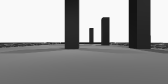
\includegraphics{Bilder/data_entry_original.png}}\\
     \subfigure[Gaussian Noise Mean 0 Sigma 5]{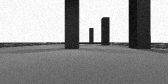
\includegraphics{Bilder/data_entry_augmented_gaussian_sigma_5.png}}\\
     \subfigure[salt-and-pepper noise]{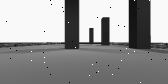
\includegraphics{Bilder/data_entry_augmented_salt_and_pepper.png}}
     \caption{Data augmentation examples}
     \label{fig:3tracks}
\end{figure}

% TODO find another paper with data augmentaton


\section{Environment Description}
\label{cha:env_description}

\subsection{Environment Simulation}
\label{sec:env_simulation}

The environment is simulated in the Unity game engine. The reinforcement learning algorithm is implemented in Python and builds upon the stable-baselines3 library. This library is able to train a proximal policy algorithm on any environment that implement the Gymnasium API. The Unity environment is wrapped in a Python class that implements the Gymnasium API. This class is responsible for the communication between the reinforcement learning algorithm and the Unity engine. The communication is implemented using JsonRPC and the Peaceful Pie \autocite{peacefulpie} library.

\paragraph{Parallel environment procesing} The stable-baselines3 library supports the parallel processing of multiple environments. The config parameter $n_envs$ specifies how many environments are simulated in parallel. The environments are simuated in the same Unity instance, see \ref{fig:parallel_simulation_unity_instance}. The seperation between the Unity engine and the Python algorithm requires JsonRPC calls for every environment step and reset. This can slow the training process. The overhead of sending calls to the Unity engine can be reduced by bundling the calls for all environments in one JsonRPC call. The $use\_bundled\_calls$ config parameter enables the bundling of calls.

\begin{figure}
    \centering
    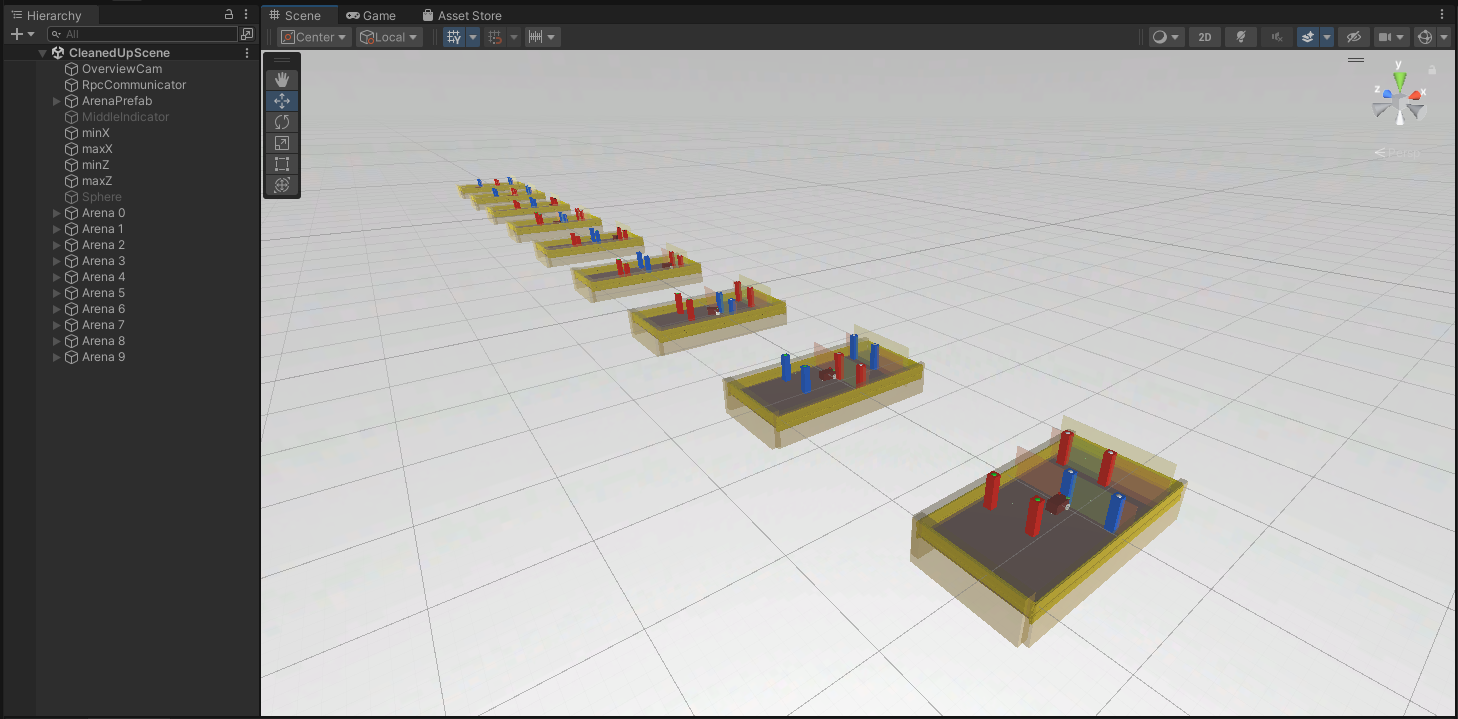
\includegraphics[width=0.8\textwidth]{Bilder/parallel_simulation_unity_instance.png}
    \caption{Parallel simulation of multiple environments in one Unity instance}
    \label{fig:parallel_simulation_unity_instance}
\end{figure}


\paragraph{Non-blocking step calls}
The step function of the Unity environment is non-blocking. This means that Unity returns the call before the entire step transition is complete. This saves time by reducing the amount of JsonRPC calls. In conventional reinforcement learning each step transition results in a new observation that is used to predict the next action. In this implementation the step call to Unity returns the observation from the start of the step instead. This observation does not capture the changes that have occurred in the environment during the step transition. The full changes are then visible to the agent after the next step has completed. Essentially the returned observation is delayed by one step or $fixedTimestepsLength seconds$. A shorter $fixedTimestepsLength$ results in smaller changes of the environment during the step transitions. In this case the delay of observations has less of an impact on the accuracy of the observations.
Experiments show that the policy can learn to deal with this delay.

Alternatively there is the policy parameter $use\_fresh\_obs$. If this parameter is set to true, the policy will request a new observation from Unity via another JsonRPC call before predicting the next action. This can be useful if the policy is sensitive to the observation delay. However this increases the amount of JsonRPC calls and can slow down the training process.

% TODO vielleicht mit einem coolen Tikz bild die blocking problematik erklären


% TODO explain the non-blocking approach of step calls here (and how the observations returned by step are delayed)
% including the use_fresh_obs flag

\begin{figure}
    \centering
    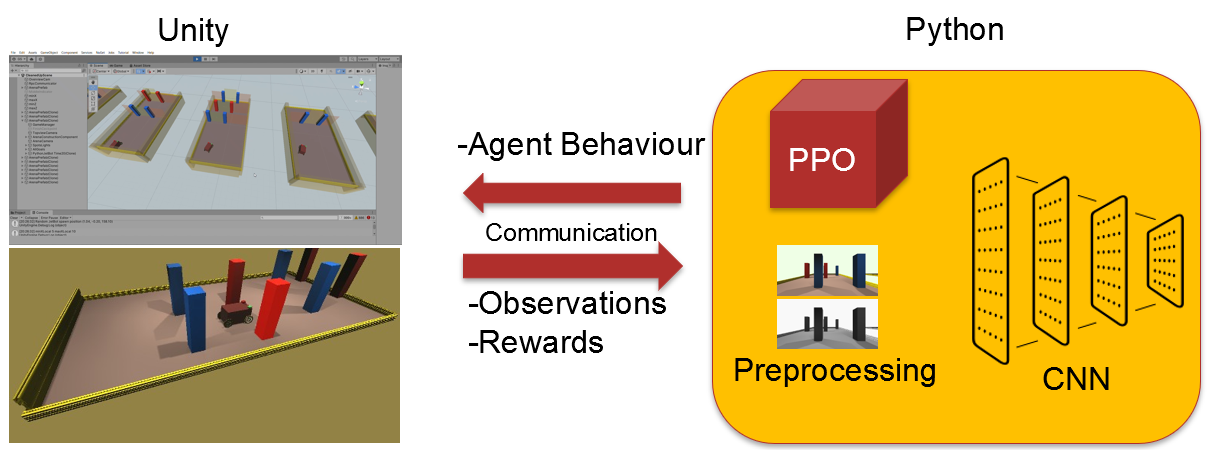
\includegraphics[width=0.4\textwidth]{Bilder/unity_communication.png}
    \caption{Communication between Python and Unity}
    \label{fig:communication_python_unity}
\end{figure} % TODO remake the image





\subsection{Arena Description}


This section describes the simulated environment and agent in detail. The environment is a 3D simulation of a physical arena at the ScaDS.AI research facility. The simulated arena consists of a rectangular platform with enclosing walls. Simulated light sources illuminate the platform from above.
The goal of our agent is to complete tracks in the arena by traversing the track's goals in order. Each goal consists of 2 cuboid pillars of the same colour. The pillars are coloured red or blue. The goals' colours alternate in the track. The distance between the pillars is fixed and the same for all goals. The positions of the goals depends on the episode's track. The tracks are grouped by the difficulty settings easy, medium and hard. An invisible finish line is positioned closely behind the last goal for each track.

\paragraph{Track Description}
The tracks in the easy setting contain 3 goals that are positioned on the arena's center line with even distances between them. The medium setting contains 3 goals that are shifted on the center line towards the arena's walls. The hard setting contains 3 goals that are shifted on the center line towards the arena's walls, resulting in a zig-zag pattern. The zig-zag pattern is the most challenging for the agent to navigate, as it requires the agent to turn sharply to pass the goals. One track from each difficulty setting is shown in figure \ref{fig:track_difficulty_settings}. The tracks in each setting are structurally very similar to each other. They differ in goal coloring and the orientation of the shift from the center line.


\begin{figure}
    \centering
    \subfigure[Easy]{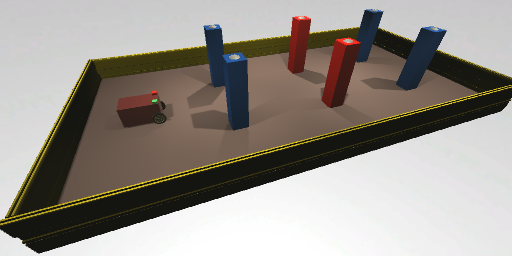
\includegraphics[width=0.3\textwidth]{Bilder/image_printer_images/evaluation_easy.png}}\qquad
    \subfigure[Medium]{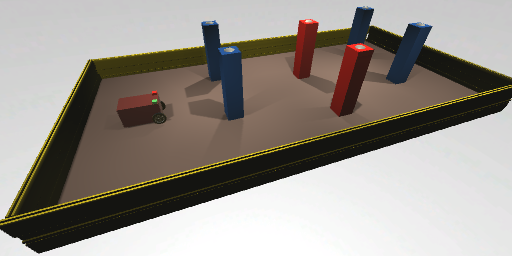
\includegraphics[width=0.3\textwidth]{Bilder/image_printer_images/evaluation_medium.png}}\qquad
    \subfigure[Hard]{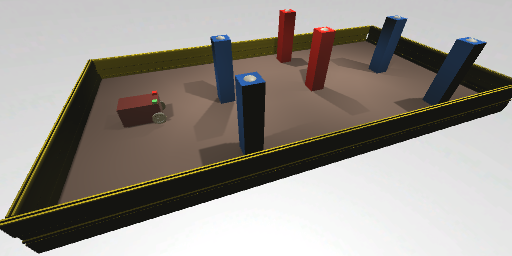
\includegraphics[width=0.3\textwidth]{Bilder/image_printer_images/evaluation_hard.png}}\\
    \caption{Example evaluation tracks for each difficulty setting.}
    \label{fig:track_difficulty_settings}
\end{figure}
% the images are generated with image_printer.py

\paragraph{Light Setting Description}
There are three light settings for the environment: bright, standard and dark. The different light settings are implemented by varying the light intensities of the arena's light sources and changing the horizon illumination of the agent's camera.

\begin{figure}
    \centering
    \subfigure[Arena Bright]{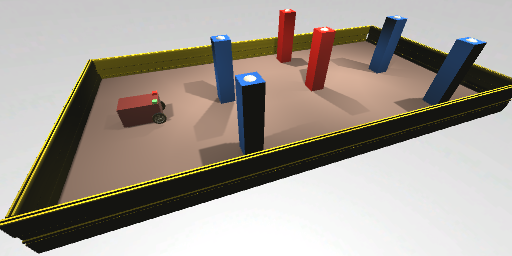
\includegraphics[width=0.3\textwidth]{Bilder/image_printer_images/light_setting_bright_arena.png}}\qquad
    \subfigure[Arena Standard]{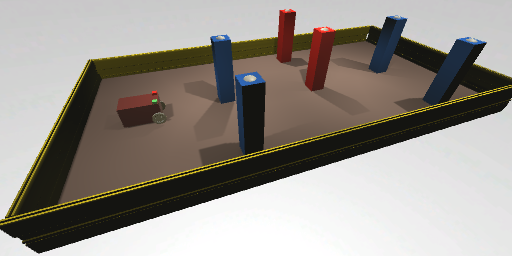
\includegraphics[width=0.3\textwidth]{Bilder/image_printer_images/light_setting_standard_arena.png}}\qquad
    \subfigure[Arena Dark]{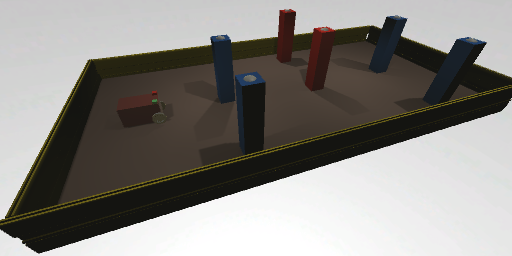
\includegraphics[width=0.3\textwidth]{Bilder/image_printer_images/light_setting_dark_arena.png}}\\
    \subfigure[Agent Bright]{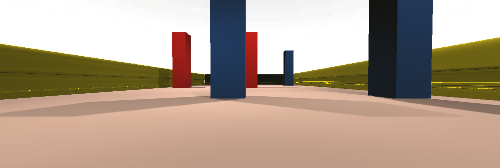
\includegraphics[width=0.3\textwidth]{Bilder/image_printer_images/light_setting_bright_pov_no_preprocessing.png}}\qquad
    \subfigure[Agent Standard]{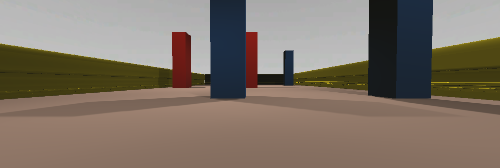
\includegraphics[width=0.3\textwidth]{Bilder/image_printer_images/light_setting_standard_pov_no_preprocessing.png}}\qquad
    \subfigure[Agent Dark]{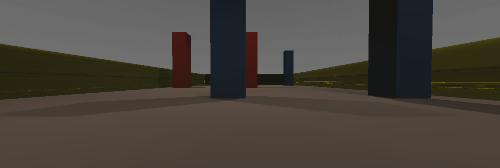
\includegraphics[width=0.3\textwidth]{Bilder/image_printer_images/light_setting_dark_pov_no_preprocessing.png}}\\
    \caption{Arena and agent camera at different light settings.}
    \label{fig:track_light_settings}
\end{figure}

\paragraph{Initial Position of Agent}
The initial position of the agent at the start of an episode is fixed. The starting position is identical for all tracks. The inital orientation is defined by the environment parameter $spawnOrientation$. The parameter specifies the range of rotations around the z-axis.There are three options for the spawnOrientation parameter: Fixed, Random and VeryRandom. For the Fixed option the agent is spawned with an orientation of 0 degrees. In the Random option the agent is spawned with an orientation between -15 and 15 degrees. In the VeryRandom option the agent is spawned with a random orientation between -45 and 45 degrees.
During the training process an orientation from the range is sampled for each episode. In the evaluation process the agent is spawned with unique orientations from the range, see \ref{sec:eval_model_track}.
The ranges for the spawnOrientation parameter influence the difficulty of completing the tracks. Depending on the spawn rotation and the selected track it might not be possible to see the entire first goal from the starting position. This is shown in \ref{fig:spawn_orientation}.


\newcommand{\spawnOrientation}[1]{\includegraphics[width=0.3\textwidth]{Bilder/image_printer_images/#1.png}}
\begin{figure}
    \centering
    \subfigure[Arena $0^{\circ}$ ]{\spawnOrientation{spawnOrientation_Fixed_max}}\qquad
    \subfigure[Arena $15^{\circ}$ ]{\spawnOrientation{spawnOrientation_Random_max}}\qquad
    \subfigure[Arena $45^{\circ}$ ]{\spawnOrientation{spawnOrientation_VeryRandom_max}}\\
    \subfigure[Agent POV $0^{\circ}$]{\spawnOrientation{spawnOrientation_Fixed_max_pov}}\qquad
    \subfigure[Agent POV $15^{\circ}$]{\spawnOrientation{spawnOrientation_Random_max_pov}}\qquad
    \subfigure[Agent POV $45^{\circ}$]{\spawnOrientation{spawnOrientation_VeryRandom_max_pov}}\qquad
    \caption{Example Spawn Orientations and agent camera views for a hard track}
    \label{fig:spawn_orientation}
\end{figure} % the figure shows that the first goal is not always visible from the starting position, very nice

\paragraph{Arena Recording}

Video recordings of episodes can be generated by the unity environment. The episode recordings are created from three different perspectives. The first perspective is the agent's camera view. This video shows the images before preprocessing steps are applied. The second perspective is a top-down view of the arena. The third perspective is a side view of the arena.
Multiple episodes can be simulated in parallel. The video recording is generally not done for all episodes due to performance problems and the large amount of data generated.
Example videos are shown in the appendix \ref{cha:example_videos}.


\subsection{Agent Description}
\label{cha:agent_description}

The agent is modeled after the NVIDIA JetBot, a small robot designed for educational purposes. The NVIDIA JetBot is equipped with a camera and a differential drive system. The agent's camera is mounted on the JetBot's front and captures the arena from the JetBot's perspective. The camera captures the arena in a 2D image format. In each step the agent receives a $leftAcceleration$ and $rightAcceleration$ value from the Python algorithm. The values range from -1 to 1 and control the agent's wheels and movement. The agent moves forward when the values are positive. When the right acceleration value is bigger the agent turns to the left and vice versa.

There are two versions of the JetBot agent in the simulation, the DifferentialJetBot and the FourWheelJetBot. The DifferentialJetBot has two driving wheels at the front and a ball supporting it at the back. The FourWheelJetBot has 2 steering driving wheels at the front and two non-driving wheels in the back. The DifferentialJetBot steers by applying different torques to the two front wheels. The two acceleration values are multiplied by a constant factor and applied to the two wheels independently.

The FourWheelJetBot steers by turning the front wheels in the desired direction and applyig equal torques to both wheels. The steering angle is computed from the difference in the two acceleration values. The torque is computed by multiplying the mean of the two acceleration values with a constant factor.
The FourWheelJetBot was used in the work by \autocite{maximilian}. The DifferentialJetBot was developed to match the physical NVIDIA JetBot more closely. The two JetBot designs are shown in figure \ref{fig:jetbots}.


\begin{figure}
    \centering
    \subfigure[Nvidia JetBot Photo]{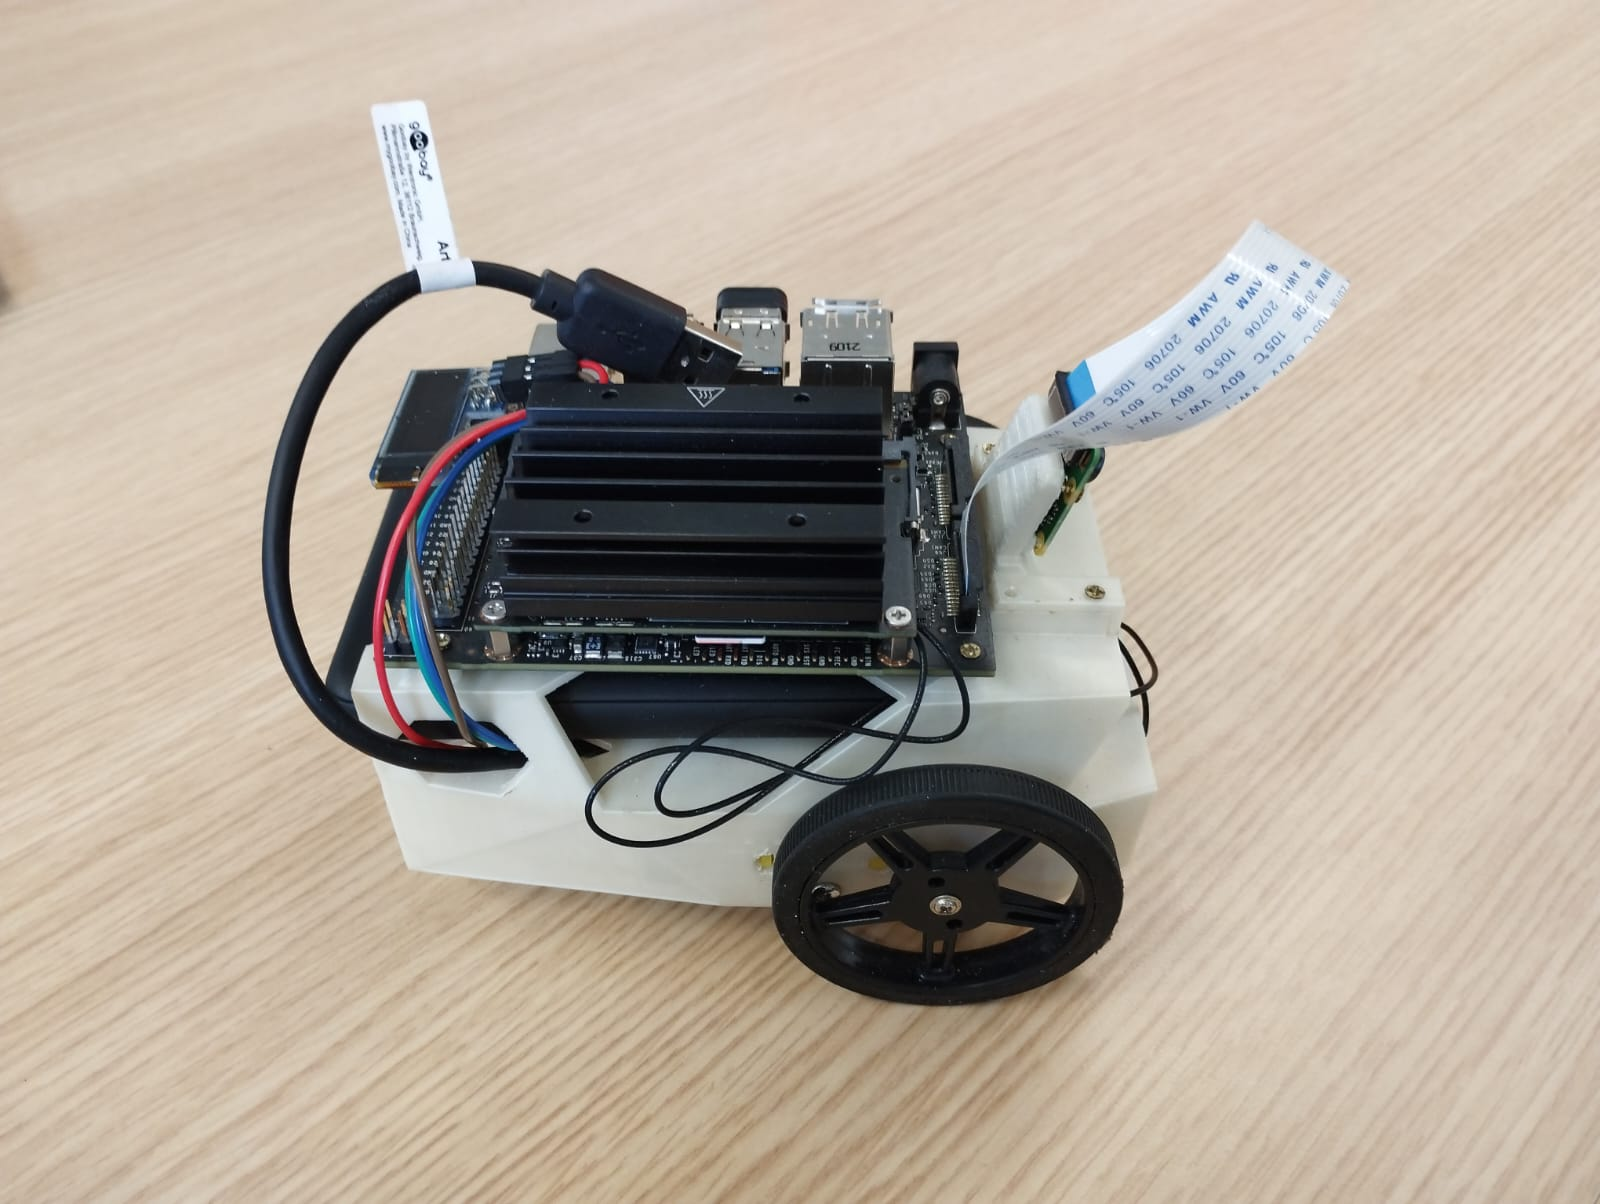
\includegraphics[width=0.3\textwidth]{Bilder/JetBotImages/NvidiaJetBot.jpeg}}\qquad
    \subfigure[DifferentialJetBot]{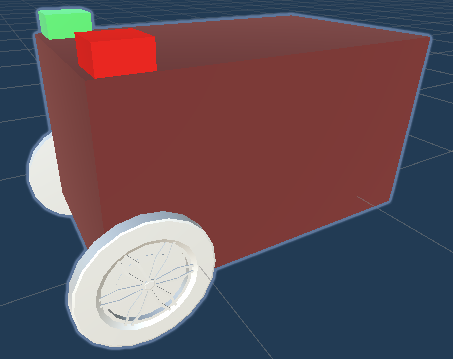
\includegraphics[width=0.3\textwidth]{Bilder/JetBotImages/DifferentialJetBot.PNG}}\qquad
    \subfigure[FourWheelJetBot]{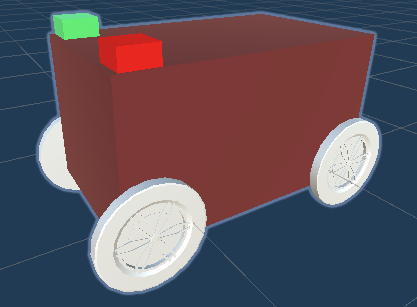
\includegraphics[width=0.3\textwidth]{Bilder/JetBotImages/FourWheelJetBot.PNG}}\qquad
    \caption{Original Nvidia JetBot and simulated JetBot Designs}
    \label{fig:jetbots}
\end{figure}


\subsection{Episode Design}

An episode represents one attempt of the agent at solving a track in the environment. Each episode consists of a series of steps starting from the initial position. Upon episode termination the end status is returned to python. This status is used to compute metrics such as the success\_rate. The agent interacts with the environment in each step. The environment is simulated in Unity during each step. This includes things like agent movement, collision detection and reward calculation.

\subsubsection{Step duration}
The duration of each step is defined by the environment settings. There are two destinct modes for the step durations. The first mode is the fixed timestep mode. In this mode the duration of each step is fixed and defined by the environment parameter $fixedTimestepsLength$. The second mode is the variable timestep mode. In this mode each step lasts until the environment receives the next action from the agent.

\paragraph{Fixed Duration}

The duration of each step is fixed in this mode. In each step the Unity environment receives an action from the policy. The environment simulation is started and the action is applied to the jetbot agent. The agent moves according to the action and interacts with the environment. The agent collects rewards, collisions and timeouts are detected. The step and environment simulation is terminated when the fixed duration has passed. The duration is defined by $fixedTimestepsLength$ in seconds. The Unity environment then waits until the next step or environment reset. The unity environment does not accept new step commands when the current step is not terminated.
An episode with fixed duration steps is shown in the upper part of figure \ref{fig:unity_timeline_steps_duration}. The figure shows how the Unity environment waits for new steps to start. The figure also shows that the waiting time may not be consistent.

The fixed mode has many advantages. The fixed duration of the steps results in consistency of the step transitions. Given identical step durations and environment state, it is well defined how the agent will move in any step. The environment state after completing a step is well defined.
Furthermore the performance of the policy does not depend on the processing speed of the device. A policy in fixed mode can be transfered to other devices without changing the policy's behaviour. In case of slower policy computation, the unity environment pauses the simulation and waits for the next step command. In case of faster policy computation, the unity environment waits until the current fixed length step is completed before starting the next step.

% TODO show an example of different step durations ? 
% show how the distance that the agent travels changes

% TODO show example steps with the 0.3 duration
% vielleicht besser bei most successful policy oder so

% TODO explain the two modes in more detail
% advantages and disadvantages of both modes


\paragraph{Variable Duration}

The duration of each step is variable in this mode. The environment simulation is started when the first step is received. In each step the Unity environment receives an action from the policy. The step's action is applied to the jetbot agent. The agent moves according to the action and interacts with the environment. The agent collects rewards, collisions and timeouts are detected. The step is terminated when a new step is received from the policy. The new step is started instantly, there is no waiting time between steps.
The duration of the steps is not fixed, it can change from step to step. It depends on the policy's computation and message transmission time. The environment simulation is not paused during the policy's computation time.
An episode with variable duration steps is shown in the lower part of figure \ref{fig:unity_timeline_steps_duration}. The figure shows how the Unity environment waits only for the first step. The figure also shows that the step sizes may change from step to step.

The biggest advantage and disadvantage this mode is that the step duration depends on the policy's computation and message transmission time. If the policy is computed fast, the average duration of the steps will be shorter. Shorter steps allow for more precise movements. Shorter durations for steps can result in a more capable policy.
A disadvantage is that the step duration can change due to a changed policy computation time. The policy computation time will be different on other devices or when there is additional load on the processing unit.
Changes in step duration might break a trained policy, as the policy has learned to expect a certain environment change for the steps. This environment change might be different for steps with different durations.
Example: The agent might decide to turn right, expecting to be able to stop the turning within 0.2 seconds. If the next step is computed too slow the agent might not be able to stop the turning in time. The agent might then crash into a wall.


\usetikzlibrary{decorations.pathreplacing}
% how to build the graphs: https://tex.stackexchange.com/questions/436259/timeline-in-latex
\definecolor{myLightGray}{RGB}{191,191,191}
\definecolor{myDarkGray}{RGB}{144,144,144}
\definecolor{myBlue}{RGB}{0,191,255}
\newcommand\offset{-3}

\begin{figure}[!ht]
    \centering
    \begin{tikzpicture}[%
            every node/.style={
                    font=\scriptsize,
                    % Better alignment, see https://tex.stackexchange.com/questions/315075
                    text height=1ex,
                    text depth=.25ex,
                },
        ]

        \node[anchor=south] at (4.25,1) {\large Fixed length time steps};

        % draw horizontal line   
        \draw[->] (0,0) -- (8.5,0);

        % draw vertical lines
        % {0,1,3,3.5,5.5,6.2,8.2}
        \foreach \x in {0,3,5.5,8.2}{
                \draw (\x cm,0.15) -- (\x cm,0);
            }
        \foreach \x in {1,3.5,6.2}{
                \draw[red] (\x cm,0.15) -- (\x cm,0); % was 3 pt and 0 pt before
            }
        % displayed fixedTimestepsLength is 2

        % place axis labels
        \node[anchor=north] at (0,0) {episode initialization};
        \node[anchor=north] at (2,0) {$t_0$};
        \node[anchor=north] at (4.5,0) {$t_1$};
        \node[anchor=north] at (7.2,0) {$t_2$};
        \node[anchor=west] at (8.5,0) {realtime};

        % draw scale above

        \fill[myLightGray] (1,0.25) rectangle (3,0.4); % step
        \fill[myLightGray] (3.5,0.25) rectangle (5.5,0.4);
        \fill[myLightGray] (6.2,0.25) rectangle (8.2,0.4);

        \fill[myBlue] (0,-0.4) rectangle (1,-0.55); % wait
        \fill[myBlue] (3,-0.4) rectangle (3.5,-0.55); % wait
        \fill[myBlue] (5.5,-0.4) rectangle (6.2,-0.55); % wait
        \draw[myBlue,dashed,thick,-latex] (8.2,-0.475) -- (8.5,-0.475);

        % draw curly braces and add their labels
        \draw[decorate,decoration={brace,amplitude=5pt}] (3.5,0.45) -- (5.5,0.45)
        node[anchor=south,midway,above=4pt] {Step};
        \draw[decorate,decoration={brace,mirror,amplitude=5pt}] (0,-0.6) -- (1,-0.6)
        node[anchor=north,midway,below=4pt] {Waiting for first step command};

        % second part
        \node[anchor=south] at (4.25, 1 + \offset) {\large Variable length time steps};
        % draw horizontal line   
        \draw[->] (0,\offset) -- (8.5,\offset);

        % draw vertical lines
        % {0,1.5,3,5.6,7.6}
        \foreach \x in {0}{
                \draw (\x cm,0.15 + \offset) -- (\x cm,0 + \offset); % was 3 pt and 0 pt before
            }

        % draw vertical lines for new step commands red
        \foreach \x in {1.5,3,5.6,7.6}{
                \draw[red] (\x cm,0.15 + \offset) -- (\x cm,0 + \offset); % was 3 pt and 0 pt before
            }

        % place axis labels
        \node[anchor=north] at (0,0+ \offset) {episode start};
        \node[anchor=north] at (2.25,0+ \offset) {$t_0$};
        \node[anchor=north] at (4.3,+ \offset) {$t_1$};
        \node[anchor=north] at (6.6,0+ \offset) {$t_2$};
        \node[anchor=north] at (8.05,0+ \offset) {$t_3$};
        \node[anchor=west] at (8.5,0+ \offset) {realtime};

        % draw scale above
        \fill[myLightGray] (1.5,0.25+ \offset) rectangle (3,0.4+ \offset); % step 0
        \fill[myDarkGray] (3,0.25+ \offset) rectangle (5.6,0.4+ \offset);
        \fill[myLightGray] (5.6,0.25+ \offset) rectangle (7.6,0.4+ \offset);
        \draw[myDarkGray,dashed,thick,-latex] (7.6,0.325+ \offset) -- (8.5,0.325+ \offset);

        \fill[myBlue] (0,-0.4+ \offset) rectangle (1.5,-0.55+ \offset); % wait for initial

        % draw curly braces and add their labels
        \draw[decorate,decoration={brace,amplitude=5pt}] (3,0.45 + \offset) -- (5.6,0.45 + \offset)
        node[anchor=south,midway,above=4pt] {Step};
        \draw[decorate,decoration={brace,mirror,amplitude=5pt}] (0,-0.6 + \offset) -- (1.5,-0.6 + \offset)
        node[anchor=north,midway,below=4pt] {Waiting for first step command};
    \end{tikzpicture}
    \begin{tabular}{r@{: }l}
        grey & step, simulation                                    \\
        blue & waiting for step command from policy, no simulation \\
        red  & new step command from policy
    \end{tabular}
    \caption{Timeline of steps in Unity for fixed and variable duration}
    \label{fig:unity_timeline_steps_duration}
\end{figure}




\subsubsection{Episode Termination}
\label{time_limit}The episodes are terminated based on the agent's interactions with the environment. Episodes are always terminated when the agent reaches the finish line or a timeout is reached. Episodes are also terminated when the agent collides with an object and the $collisonMode$ parameter is set to $terminate$.
The timeout is defined by a fixed timelimit of 30 seconds which is increased by further 30 seconds for each passed goal. The timelimit is necessary to terminate episodes where the agent does not reach the finish line. This can be due to the policy's learned behaviour or collisions.

The episode termination status is used by the python algorithms to evaluate the agent performance. The possible termination statuses are:

\paragraph*{Success}

The episode is considered to have been terminated successfully if the agent passed all of the track's goals in order.

\paragraph*{Timeout}

The timeout status is returned when the agent does not reach the finish line within the timelimit and not all goals have been passed successfully.

\paragraph{FinishWithoutAllGoals}

The FinishWithoutAllGoals status is returned when the agent reaches the finish line without passing through all goals.

\paragraph*{Collision}

Collisions of the agent with the goal posts and the arena walls are detected by the environment. The environment parameter $collisionMode$ defines how the agent's collisions are handled. The termination status Collision is returned when the agent collides with an object and the $collisionMode$ parameter is set to $terminate$.




% time-limit, episode termination, step-function, Collisions, rewards

% time limit explain here

% success is now defined as passing all three goals  (without necessarily reaching the finish line)
% this was done as the agent sometimes learns to move back and forth in front of the finish line


\subsection{Reward Function}

The reward function is a function that maps state-action pairs to a scalar reward. The reward function assigns rewards to the agent based on its actions in the environment. The reinforcement learning algorithm trains the agent to maximise the cumulative reward over an episode. The reward function is a critical component of the reinforcement learning process. It is important to design a reward function that is closely alligned with the goal. The agent could learn unintended behaviour if the reward function is not designed carefully.

\paragraph*{Event Reward}
The goal of the training process is to achieve an agent that traverses the tracks without collisions and passed through the goals in order. The eventReward function describes this behaviour \ref{fig:eventReward_function}. The event reward function is evaluated in each step. A positive reward is awarded to the agent in case it passes a goal or reaches the finish line during the step. A penalty is applied in case the agent misses a goal, collides with an object or the timeout is reached. The magnitude of ... increased TODO why, experimentation?

The maximum amount of reward obtainable from this function per episode is $num_goals * goal_reward + parcour_reward = 3 * 100 + 100 = 400$. An agent that maximises the eventReward function will complete the track without collisions. In theory the event Reward should be enough to train an agent that traverses the tracks successfully without collisions.


% TODO explain why positive rewards higher

% TODO check if a successful model reaches an average prescale event reward of 400

\begin{figure}
    \centering
    \begin{align}
        EventReward(s_t, a_t) & = \begin{cases}
                                      100,           \text{completed the parcour}           \\
                                      100,             \text{passed a goal}                 \\
                                      -1,            \text{missed a goal}                   \\
                                      -1,            \text{collision with wall or obstacle} \\
                                      -1,            \text{timeout}                         \\
                                      0,             \text{otherwise}                       \\
                                  \end{cases} \nonumber
    \end{align}
    \caption{Event Reward function}
    \begin{tabular}{r@{: }l r@{: }l}
        $s_t$ & state t & $a_t$ & action in state t
    \end{tabular}
    \label{fig:eventReward_function}
\end{figure}


\paragraph*{Dense Reward Functions}
The eventReward function provides the agent with a reward signal that is closely aligned with the desired behaviour. However the eventRewards are only awarded in very few steps. In the optimal episode there are only 4 steps where the reward is non-zero. Three steps where the agent passes a goal and one step where the agent reaches the finish line. The eventReward function is a sparse reward function. Sparse rewards can make it difficult for the agent to learn the desired behaviour. In the case of the eventReward, the agent might never learn to drive towards a goal since there are no rewards that encourage that behaviour. The agent would rely on random exploration alone to discover the positive reward associated with successfully driving through a goal.
Additional reward functions were developed to help the agent learn to complete the tracks. The additional reward functions are dense reward functions. They assign non-zero rewards in most steps. This is comparable to encouraging route following behaviour with a trail of candy versus a big cake at the end of the route.


Dense rewards functions can exasterbate the issue of the agent learning unintended behaviour. The dense rewards can be opinionated and encourage the agent to follow a very specific path. This can lead to the agent not exploring the environment enough to find the very best policy. This is to be kept in mind when designing and testing the dense reward functions.

% TODO dicuss the diasdvantage of dense reward functions
% TODO discuss the issue of the dense rewards being opinionated?
% distanceReward encourages the agent to pass the goal through the middle. that is not necessary for the desired behaviour.
% it is also not the most  optimal line driving through the middle of the goal posts
% but this might not translate to the agent's behaviour

\paragraph{Velocity Reward}
The first dense reward function is the velocityReward. It was already developed in previous work \autocite{maximilian} to encourage the agent to drive at full speed. The velocityReward function assigns a reward proportional to the agent's velocity. The reward from driving forward might also help at discovering other rewards, e.g. the positive reward for passing a goal awared by eventReward function.

\paragraph{Orientation Reward}
The second dense reward function is the orientationReward. The orientationReward function assigns a reward based on the agent's orientation. The reward is proportional to the cosine similarity between the agent's orientation and the direction towards the next goal. The orientationReward function encourages the agent to face the next goal. Together with other rewards this can help teach the agent to drive through the next goal.

\paragraph{Distance Reward}
The third and last dense reward function is the distanceReward function. The distanceReward function assigns a reward proportional to the difference in distance between the agent and the next goal. The distanceReward is positive if the agent gets closer to the next goal during a step transition. The distance to the next goal is measured from the midpoint between the two goal posts. The distanceReward function encourages higher driving velocity, as higher velocities result in bigger distance differences and thus rewards. The distanceReward function also encourages the agent to drive strait towards the next goal, as this results in the biggest distance differences. In theory the agent should be able to learn to complete the tracks successfully from the distanceReward alone.

The distance reward is opinionated. It guides the agent towards the midpoint of the next goal. This reward signal may result in a suboptimal path for the agent. The agent might learn to drive through the goal posts at the midpoint. This is not necessary for the desired behaviour. This is a tradeoff that was made when designing the distance reward function.
% opinionated was also discused above at intro of dense reward functions

\paragraph{Composite Reward Function}
The four individual reward functions can be combined in many ways to give the agent dense and meaningful rewards. In previous work the eventReward was combined with the velocityReward to train the agent. In this work we combine the individual reward functions in the composite reward function \ref{fig:reward_functions}. The composite reward function applies scalar weights to the individual reward functions and returns this weighted sum of rewards to the agent. It is crucial to select an appropriate combination of weights for the individual reward functions during training. The weights determine the importance of the individual reward functions and can influence the learned behaviour. If the velocityReward is weighted too high the agent might learn to drive at full speed in circles without ever reaching the finish line. It is also to note that setting a specific reward function's weight to zero essentially removes that reward function.

\begin{figure}
    \centering
    \begin{align}
        R(s_t,a_t)                 & = c_1 \cdot DistanceReward(s_t,a_t) + c_2 \cdot OrientationReward(s_t,a_t) \nonumber \\
                                   & + c_3 \cdot VelocityReward(s_t, a_t) + c_4 \cdot EventReward(s_t, a_t) \nonumber     \\
        DistanceReward(s_t,a_t)    & = \Delta distance(Agent, NextGoalPosition) \cdot \Delta T \nonumber                  \\
        OrientationReward(s_t,a_t) & = S_C(NextGoalPosition - AgentPosition, agentDirection) \cdot \Delta T \nonumber     \\
        VelocityReward(s_t, a_t)   & = v \cdot \Delta T \nonumber                                                         \\
        EventReward(s_t, a_t)      & = \begin{cases}
                                           100,           \text{completed the parcour}           \\
                                           1,             \text{passed a goal}                   \\
                                           -1,            \text{missed a goal}                   \\
                                           -1,            \text{collision with wall or obstacle} \\
                                           -1,            \text{timeout}                         \\
                                           0,             \text{otherwise}                       \\
                                       \end{cases} \nonumber
    \end{align}
    \caption{Complete reward function R with all its components}
    \begin{tabular}{r@{: }l r@{: }l}
        $S_C$ & cosine similarity & $c_i$ & weights           \\
        $s_t$ & state t           & $a_t$ & action in state t
    \end{tabular}
    \label{fig:reward_functions}
\end{figure}
% cosine similarity is one for same direction, zero for orthogonal directions and -1 for opposite directions



\subsection{Collision Mode}

The variable $collisionMode$ describes how the environment handles collisions of the agent with the goal objects and walls. The $collisionMode$ can take 5 different values described in table \ref{fig:collision_modes}. In previous research the episodes were terminated upon collision and when missing a goal \autocite{maximilian}. Furthermore there existed two different training regimes. The first regime trained the agent on the full maps, while the second regime trained the agent on a map with only one goal.

The $collisionMode$ parameter was introduced to allow for more flexibility in the training process and fine control over the event rewards. The inital implementation was the unrestricted mode. Training with the unrestricted mode and event reward showed that the agent's policy started out with extreme negative rewards. The agent quickly learned to avoid these negative rewards by avoiding all collisions and movements. The policy got stuck in a local optimum \ref{fig:event_reward_only_collisionModeUnrestricted_event_reward}.The policy did not learn to complete the parcour during the remainder of training. The unrestricted mode potentially triggers the collision's negative rewards multiple times per step. This results in a big skew of the eventReward function towards negative rewards.

\begin{figure}
    \centering
    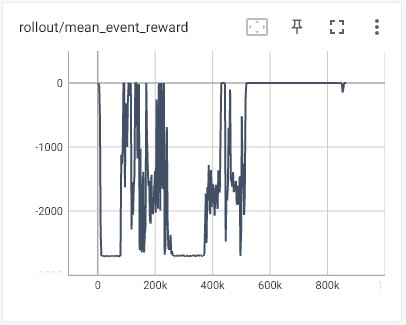
\includegraphics[width=0.3\textwidth]{Bilder/tensorboard_images/eventRewardOnly_collisionModeUnrestricted_eventReward.png}
    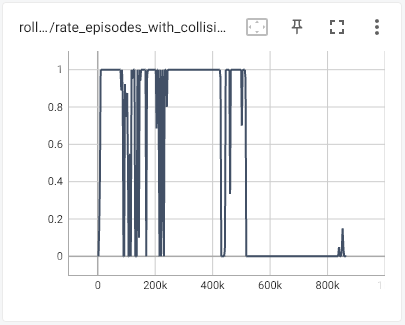
\includegraphics[width=0.3\textwidth]{Bilder/tensorboard_images/eventRewardOnly_collisionModeUnrestricted_collisionRate.png}
    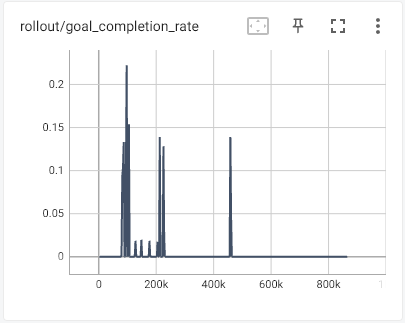
\includegraphics[width=0.3\textwidth]{Bilder/tensorboard_images/eventRewardOnly_collisionModeUnrestricted_goalCompletionRate.png}
    \caption{Event Reward only training with $collisionMode$ $unrestricted$}
    \label{fig:event_reward_only_collisionModeUnrestricted_event_reward}
\end{figure}

The modes $oncePerTimestep$, $oncePerTimestep$, $terminate$ and $ignore$ were introduced to limit the negative rewards caused by collisions. Reducing the negative rewards could lead to a policy that does not avoid collisions and movement as much as. This could lead to more exploration of the environment and a succesful policy.

% maximilian ended the episode on collision and on goal missed https://github.com/Maddi97/master_thesis/blob/main/carsim/Assets/Scripts/CheckpointManager.cs


\begin{figure}

    \begin{center}
        \begin{tabular}{|| p{0.2\linewidth} | p{0.35\linewidth} | p{0.35\linewidth} ||}
            \hline
            collisionMode   & \makecell{Behaviour upon Collision}                                                                                        & Reasoning                                                                                \\ [0.5ex]
            \hline\hline
            unrestricted    & Negative reward is given for each frame with collision.  This can result in multiple penalties given during a single step. & Default behaviour                                                                        \\
            \hline
            oncePerTimestep & Negative reward for collisions is given only once per step.                                                                & Limits the negative reward caused by a collision in a step.                              \\
            \hline
            oncePerEpisode  & Negative reward for collision is only given once  per episode per object.                                                  & Limits the negative reward caused by ongoing collisions.                                 \\
            \hline
            terminate       & Episode is terminated instantly.                                                                                           & No ongoing collisions. The early termination could speed up the neural network training. \\
            \hline
            ignore          & Collisions are ignored, no negative reward is given.                                                                       & The agent might learn to avoid collisions based on other rewards.                        \\
            \hline
        \end{tabular}
    \end{center}
    \caption{Collision Modes}
    \label{fig:collision_modes}
\end{figure}




\section{Policy}
\label{fig:policy_description}

The policy dictates the agent's behaviour. The policy is responsible for selecting actions from observations. The policy is trained using the \ac{PPO} algorithm. The algorithm has proven to be very reliable \textcite{ppo}. The algorithm can be used for our continuous control task.

A neural network is used as for the policy here. The neural network belongs to the class of \acp{CNN}. This architecture was chosen since convolutional neural networks are ideal for processing image data. The convolutional network's architecture follows the specifications from \textcite{human_level_control}. This architecture has been used successfully in comparable reinforcement learning control tasks.

The network takes the output of the observation preprocessing as input. This input is a three dimensional tensor, similar to an image. The network consists of convolutional and fully connected layers. The network produces two outputs, an action distribution and a value function. The action distribution is a probability distribution over the action space.
The value function is a scalar value that estimates the expected return of the current state. The value function is not used during the action inference. The value is only used during the training of the policy network. It is used to compute the advantage function which is required for the loss in \ac{PPO} \textcite{ppo}.

% value or is it the critic? --> it is value


% human_level_control definiert das NatureCNN welches wir nutzen um die features zu extrahieren
% human_level_control hat einfaches Q-learning verwendet, nicht PPO



\subsubsection{Observation Space}

The input space of the neural network is three dimensional. The input is structured like images with $width$, $heigth$ and $channel$ dimensions. The dimensions are determined by the agent's camera image dimensions, preprocessing parameters and the memory mechanism. The input space is a tensor with the following dimensions:

\begin{align*}
    width    & = \frac{agentImageWidth}{downsampling\_factor}  \\
    height   & = \frac{agentImageHeight}{downsampling\_factor} \\
    channels & = frame\_stacking \cdot num\_color\_channels
\end{align*}

The tensor values are integers in the range $[0,255]$. Storing the pixel intensities as integers saves a lot of memory compared to floats.


\subsubsection{Action Space}

The environment's action space is two dimensional, the dimensions are called $leftAcceleration$ and $rightAcceleration$. The values are restricted to the range $[-1,1]$ and dictate the agent movement \ref*{cha:agent_description}.

\subsubsection{Architecture}
\label{sec:network_architecture}

The neural network has an action and a value head. The action head produces the action distribution. The value head produces an estimate of the state's value. 

The action and value head share the first part of the neural network. The shared part is called the feature extractor and consitutes the first four layers. The feature extractor consists of three convolutional layers and one fully connected layer. The first convolutional layer takes the output of the memory buffer as input. The output of the feature extractor's fully connected layer is used by the action and value heads.


\paragraph{Action Head}
\label{sec:action_sampling}

The action head consists of a single fully connected layer with two outputs. The two outputs represent the mean of the action distribution. The action distribution is a Gaussian Distribution. The action distribution can be sampled deterministically or stochastically to obtain an action for the agent. The most likely action is returned in determinsitc sampling. This is equal to the outputs of the action head. In stochastic sampling, the action is sampled from the action distribution.

The sampled actions are clipped to the output space's range $[-1,1]$. This is necessary as the sampling can return a value outside of the range.

\paragraph{Value Head}
The value head consists of a single fully connected layer with one scalar output.

\begin{figure}[!h]
    \centering
    \begin{tikzpicture}[%
            every node/.style={
                    font=\scriptsize,
                    % Better alignment, see https://tex.stackexchange.com/questions/315075
                    text height=1ex,
                    text depth=.25ex,
                }, outer sep=auto
        ]

        \node[draw] (input) at (0, 0) {Input image stack [width, height, channels]};

        \node[draw] (c1) at (0, -1) {Convolutional Layer 1};
        \node[draw] (c2) at (0, -2) {Convolutional Layer 2};
        \node[draw] (c3) at (0, -3) {Convolutional Layer 3};
        \node[draw] (fc1) at (0, -4) {Fully Connected Layer};

        \draw[decorate,decoration={brace,amplitude=5pt}] (3.5,-1) -- (3.5,-4)
        node[anchor=west,midway,right=4pt] {Feature Extractor};

        \node[draw] (fcAction) at (-2, -5.5) {Fully Connected Layer};
        \node[draw] (actionDist) at (-2, -6.5) {Action Distribution};
        \node[draw] (actionOut) at (-2, -7.5) {Action Output};

        \node[draw] (fcValue) at (2, -5.5) {Fully Connected Layer};
        \node[draw] (valueOutput) at (2, -6.5) {Value Output};

        \draw[decorate,decoration={brace,mirror,amplitude=5pt}] (-4,-5.5) -- (-4,-7.5)
        node[anchor=east,midway,left=4pt] {Action Head};

        \draw[decorate,decoration={brace,amplitude=5pt}] (4,-5.5) -- (4,-6.5)
        node[anchor=west,midway,right=4pt] {Value Head};

        \draw[->,thick] (input.south) -- (c1.north);
        \draw[->,thick] (c1.south) -- (c2.north);
        \draw[->,thick] (c2.south) -- (c3.north);
        \draw[->,thick] (c3.south) -- (fc1.north);

        \draw[->,thick] (fc1.south) -- (fcAction.north);
        \draw[->,thick] (fcAction.south) -- (actionDist.north);
        \draw[->,thick] (actionDist.south) -- (actionOut.north);

        \draw[->,thick] (fc1.south) -- (fcValue.north);
        \draw[->,thick] (fcValue.south) -- (valueOutput.north);

    \end{tikzpicture}
    \caption{Neural Network Structure}
    \label{fig:network_structure}
\end{figure}


\subsubsection{Parameters}
The neural network's input dimensions are determined by the agent's camera image dimensions and the observation processing. The network architecture follows the specifications from \textcite{human_level_control}. However the observation space differ from their network. This results in a different number of parameters for the feature extractor's layers.
The parameters and layer dimensions used network are shown in figure \ref{fig:network_architecture}.


% verified in code:
% action and value head share the extractor
% when sampling deterministic, the action is the mean of the distribution
% the output of the action head is the mean of the distribution

% the action head is a single linear layer, there is no activation function applied to the output

% DiagGaussianDistribution
% the log std of the distribution is a learnable parameter
% it is also updated, see policy_loss (the single parameter of size 2 that is added in the graph last)

\begin{figure}
    \begin{center}
        \begin{tabular}{|| c | p{0.25\linewidth} | p{0.4\linewidth} ||}
            \hline
            Component                          & Layer Type            & Layer Specifications                     \\ [0.5ex]
            \hline\hline
            \multirow{4}{*}{Feature Extractor} & Convolutional Layer   & 32 filters, 3 dimensional (10, 8, 8)     \\\cline{2-3}
                                               & Convolutional Layer   & 64 filters, 3 dimensional (32, 4, 4)     \\\cline{2-3}
                                               & Convolutional Layer   & 64 filters, 3 dimensional (64, 3, 3)     \\\cline{2-3}
                                               & Fully connected Layer & 512 output neurons, (512 x 12096) matrix \\
            \hline
            Action Head                        & Fully connected Layer & 2 output neurons, (2 x 512) matrix       \\
            \hline
            Value Head                         & Fully connected Layer & 1 output neuron, (1 x 512) matrix        \\
            \hline
        \end{tabular}
        \begin{tabular}{r@{: }l}
            $agentImageWidth$      & 500  \\
            $agentImageHeight$     & 168  \\
            $downsampling\_factor$ & 2    \\
            $greyscale$            & True \\
            $equalize$             & True \\
            $frame\_stacking$      & 10   \\
        \end{tabular}
    \end{center}
    \caption{Neural network layers and parameters for the best configuration}
    \label{fig:network_architecture}
\end{figure}



\section{Training Algorithm}

% mention the best_model during collect_rollouts
% mention this is because the real full eval is expensive


The policy training process consists of a simple training loop. In each iteration, the algorithm collects data from the environment. The data is stored in a replay buffer. After collecting the data, the model is trained on the data in the replay buffer. The training process is repeated until a certain number of timesteps has been collected.  

In most \ac{RL} algorithms, the trained model's performance is evaluated at short intervals. The frequent evaluations serve as a way to monitor the model's performance during training and measure progress. It is not guaranteed in \ac{RL} that a model improves during each model update. Therefore frequent evaluations also help in finding the best version of the model.  
In this training algorithm there is no dedicated evaluation process at short intervals. Instead the episodes from the data collection step are used to evaluate the model at every iteration of the training loop. This saves computational resources compared to a dedicated evaluation of the model.

\renewcommand{\thepseudonum}{\roman{pseudonum}}
\begin{pseudocode}{TrainNetwork}{ }
\label{train_network}
\COMMENT{Main Training Algorithm}\\

\MAIN
Env \GETS \CALL{Environment}{environment\_parameters}\\
RolloutBuffer \GETS \CALL{RolloutBuffer}{rollout\_buffer\_size}\\
Model \GETS \CALL{Model}{model\_parameters}\\
Optimizer \GETS \CALL{Optimizer}{optimizer\_parameters}\\

num\_timesteps \GETS 0\\
\WHILE num\_timesteps < total\_timesteps \DO 
\BEGIN 
num\_collected\_steps \GETS \CALL{CollectData}{}\\
num\_timesteps \GETS num\_timesteps + num\_collected\_steps\\
\CALL{TrainModel}{}\\
\END\\
\ENDMAIN
\end{pseudocode}

\subsection{Collect Data}

The data is stored in a replay buffer for use by the training algorithm. The data collection process starts by resetting the replay buffer, this removes the collected sampled of previous iterations from memory.
The data collection process is a simple loop that collects a fixed amount of samples from the environment. The \ac{PPO} \ac{RL} algorithm requires that the samples are collected on-policy. As a result the most recently updated model is used to chose actions during the data collection. 

The data collection algorithm starts a new episode and applies the policy to the environment until the episode terminates. The observation is used to prompt the \ac{CNN} policy for an action. The action is then applied to the environment, resulting in a reward and a new environment state. The observation, action and reward tuples are stored in the replay buffer. A new episode is started upon termination of the current episode. The data collection process continues until the replay buffer is full.

Actions are sampled non-deterministically from the policy. This ensures that the agent explores the environment and is able to learn from new data.

\paragraph{Environment settings for Data collection}

The environment settings define how the episodes are reset during the data collection process. The episodes are initialized according to the parameters trainingMapType, trainingLightSetting and spawnOrientation \ref{fig:env_reset_settings}. The settings influence the difficulty and variety of the tracks. The settings define what data the agent policy can learn from during training.

Different configurations are used in the experimentation phase to gain insights into the network's capabilities.


\begin{figure}
    
    \begin{center}
    \begin{tabular}{|| c | p{0.25\linewidth} | p{0.4\linewidth} ||} 
        \hline
        Parameter name & Options & Explanation  \\ [0.5ex] 
        \hline\hline
        \multirow{4}{*}{trainingMapType} & randomEvalEasy & Selects a random easy track. \\\cline{2-3}
        & randomEvalMedium & Selects a random medium track. \\\cline{2-3}
        & randomEvalHard & Selects a random hard track. \\\cline{2-3}
        & randomEval & Selects a random track from all difficulties. 20\% easy, 40\% medium, 40\% hard \\
        \hline
        \multirow{4}{*}{trainingLightSetting} & bright & Bright illumination. \\\cline{2-3}
        & standard & Standard illumination. \\\cline{2-3}
        & dark & Dark illumination. \\\cline{2-3}
        & random & Selects a random light setting from bright, standard and dark. \\
        \hline
        \multirow{4}{*}{spawnOrientation} & Fixed & Spawn JetBot with fixed coordinates and orientation. \\\cline{2-3}
        & Random & Spawn JetBot with fixed coordinates and random orientation (-15 to 15 degrees). \\\cline{2-3}
        & VeryRandom & Spawn JetBot with fixed coordinates and random orientation (-45 to 45 degrees). \\
        \hline
    \end{tabular}
    \end{center}
    \caption{Environment parameters for training.} % the parameters are already defined in endDescription
    \label{fig:env_reset_settings}
\end{figure}

\paragraph{Evaluation of the model}

There is no dedicated evaluation step in this training algorithm. The collected episodes are analysed to gain insight into the policy's performance during training. No episodes are executed solely for the purpose of measuring the policy's performance during training. The full evaluation of the model as described in \ref{sec:basic_evaluation_algorithm} is time-consuming. The full evaluation process is only executed after the training process has finished, this speeds up training tremendously.

The collected episodes are used to evaluate the model during training. The success rate of the collected episodes is used to determine the best model. The model is saved to disk if the success rate of the collected episodes improved.


The success\_rate and other statistics about the collected episodes are logged to tensorboard to monitor the training process. Example metrics are the goal\_completion\_rate and the collected weighted rewards.
These metrics can show how the policy behaves over time. They show if the policy is able to learn from the collected episodes \ref{fig:metrics_over_time}.

\begin{figure}
    \centering
    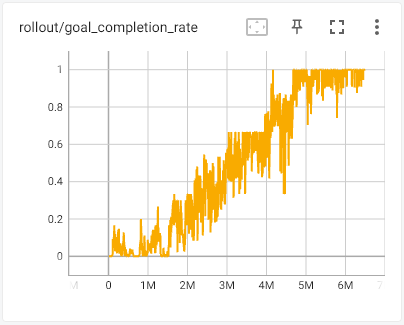
\includegraphics[width=0.4\textwidth]{Bilder/tensorboard_images/successfulTraining_goal_completion_rate.png}
    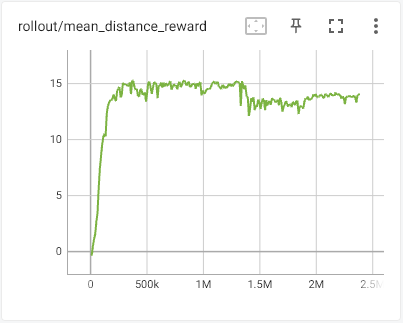
\includegraphics[width=0.4\textwidth]{Bilder/tensorboard_images/successfulTraining_distance_reward.png}
    \caption{Metrics from collected episodes during a successful training}
    \label{fig:metrics_over_time}
\end{figure}


\subsection{Train Model}

The model training part of the algorithm is very conventional and follows the standard implementation of \ac{PPO} training. The model is trained on the collected data for a fixed number of epochs. In each epoch the replay buffer is sampled to create batches of data. The loss is computed for each batch. The gradient of the weights with respect to the loss is computed using backpropagation. The optimizer is then used to update the model parameters using the gradients.

The entire data from the replay buffer is sampled in every epoch. This ensure that the collected data is used efficiently. The data is shuffled before creating the batches. This ensures that the samples are less correlated and the model updates are more stable.
% the \ac{PPO} paper uses gradient ascent

\subsubsection*{Loss function}

The loss function follows the \ac{PPO} algorithm by \textcite{ppo}. The \ac{PPO} loss function is a combination of the policy surrogate and value error. The policy surrogate and value error are combined to be able to update the weights of the entire \ac{NN} together.

The policy surrogate objective function is responsible for improving the policy's output action distribution. The function behaves similarly to other policy update based aproaches. It restricts the size of parameter updates, increasing the stability during training. The ratio between the old and the current policy is clipped. The clipped ratio and non-clipped ratio are multiplied by the advantage. The minimum of the two is used as the policy surrogate loss. This prevents the updates from changing the policy drastically.

The advantage is an estimator for how much better (or worse) the policy performed than expected. The advantage $\hat{A}_t$ is computed using the value estimates produced by the \ac{NN}. The multiplication of the ratio with the advantage leads to increased probabilities for good actions and decreased probabilities for bad actions.

The value error is responsible for improving the policy's output value estimates. The value error is the mean squared error between the predicted value and the target value. The parameter changes caused by the value error lead to a more accurate value prediction.

The policy loss can also include an entropy term. Similarly to the original paper \textcite{ppo}, no entropy term is used in this work. This results in the loss function \eqref{eq:eq1} with the value coefficient $c_1 = 0.5$.

\begin{align*}
    L_t^{CLIP + VF} &= \hat{\mathbb{E}}_t [L_t^{CLIP}(\theta) - c_1 L_t^{VF}(\theta)] \label{eq:eq1}\tag{\ac{PPO} Loss} \\
    L_t^{CLIP}(\theta) &= min(r_t(\theta)\hat{A}_t, clip(r_t(\theta), 1-\epsilon, 1+\epsilon)\hat{A}_t) \label{eq:eq2}\tag{Surrogate Objective}\\
    r_t(\theta) &= \frac{\pi_\theta(a_t|s_t)}{\pi_{\theta_{old}}(a_t|s_t)} \label{eq:eq3}\tag{Ratio}\\
    L_t^{VF}(\theta) &= (V_\theta (s_t) - V_t^{targ})^2 \label{eq:eq4}\tag{Value Error}
\end{align*}
% for the target value + advantage computation see my_buffers.compute_returns_and_advantage returns

\subsection{Final Result of Training Algorithm}

Weight updates can lead to a decrease in performance during the training process. The model after the final weight update is not guaranteed to be the best observed version.
The model performance is evaluated during training using the collected episodes. The model with the highest observed success\_rate is considered to be the final output of the training algorithm. This model is later used for the full evaluations.



\chapter{Experiment Description}
\label{cha:Experiments}

\section{Evaluation metrics}

\subsection{success\_rate}
The primary metric of evaluation for the developed agents is the $success\_rate$. The $success\_rate$ is defined as the ratio of successful episodes to the total number of episodes. An episode is considered successful if the agent passes through all three goals within the time limit \ref{time_limit}. Collisions of the agent do not disqualify an episode from being succesful, as long as the agent passes all goals.

\subsection{goal\_completion\_rate}

The $goal\_completion\_rate$ is defined as the ratio of passed goals to the total number of goals in the episodes. The $goal\_completion\_rate$ is a more fine-grained metric than the $success\_rate$. However the two metrics are closely related as a high $success\_rate$ implies a high goal\_completion\_rate. The major advantage of the $goal\_completion\_rate$ is that it can used to measure the progress of an agent during training more accurately.
The $goal\_completion\_rate$ would increase when the agent is able to pass more goals on average, whereas the $success\_rate$ would only increase when the agent is able to pass all goals in an episode more often. The $goal\_completion\_rate$ captures learning progress earlier in training. This behaviour can be observed in training runs, shown in \ref{fig:success_rate_vs_goal_completion_rate}.


\begin{figure}
    \centering
    \subfigure[success\_rate]{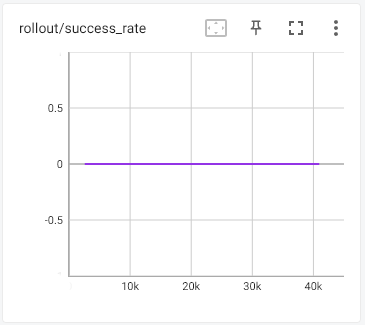
\includegraphics[width=0.3\textwidth]{Bilder/metrics/sr_vs_gcr_success_rate.PNG}}
    \subfigure[goal\_completion\_rate]{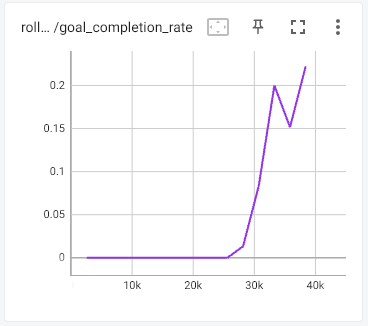
\includegraphics[width=0.3\textwidth]{Bilder/metrics/sr_vs_gcr_goal_completion_rate.PNG}}
    \caption{Difference in success rate and goal completion rate during early stages of training.}
    \label{fig:success_rate_vs_goal_completion_rate}
\end{figure}
% diese Bilder funktionieren nur für frühe Episoden, später sind die Werte sehr gleich

\subsection{collision\_rate}

The $collision\_rate$ is defined as the ratio of episodes with one or more collisions to the total number of episodes. The $collision\_rate$ is a measure of the agent's ability to avoid obstacles. The $collision\_rate$ is a secondary metric. The $collision\_rate$ is used in combination with the $success\_rate$ to determine the agent's performance.
The collision rate is also very useful during the training of the agent. If the agent's goal completion rate is low and there are no collisions, the agent might be stuck in a local optimum. In one such situation, the agent turned on the spot avoiding any collisions and did not move forward at all.
The collision rate can be used to detect such situations, the training process can then be adjusted accordingly.


\section{Basic evaluation algorithm}
\label{sec:basic_evaluation_algorithm}

This section explains the most important component of the evaluation algorithms. It explains how the policy's performance is evaluated on a specific light and difficulty setting. The sampling mode, jetbot name and other policy parameters can also be specified \ref{table:basic_eval_algorithm_parameters}. This basic component is widely used in the following tests.


\begin{table}
    \begin{center}
        \begin{tabular}{|| c | p{0.20\linewidth} | p{0.4\linewidth} ||}
            \hline
            Parameter name                     & Options              & Explanation                                                                                  \\ [0.5ex]
            \hline\hline
            \multirow{1}{*}{n\_eval\_episodes} & any positive integer & Amount of episodes to use for evaluation                                                     \\
            \hline
            \multirow{3}{*}{difficulty}        & easy                 & \multirow{3}{\linewidth}{Determines tracks used for episodes}                                \\\cline{2-2}
                                               & medium               &                                                                                              \\\cline{2-2}
                                               & hard                 &                                                                                              \\
            \hline
            \multirow{3}{*}{light\_setting}    & bright               & \multirow{3}{\linewidth}{Determines light setting for episodes}                              \\\cline{2-2}
                                               & standard             &                                                                                              \\\cline{2-2}
                                               & dark                 &                                                                                              \\
            \hline
            \multirow{2}{*}{jetbot\_name}      & DifferentialJetBot   & \multirow{2}{\linewidth}{JetBot version for episodes}                                        \\\cline{2-2}
                                               & FourWheelJetBot      &                                                                                              \\
            \hline
            \multirow{2}{*}{deterministic}     & True                 & \multirow{2}{\linewidth}{If True, use deterministic sampling for policy actions}             \\\cline{2-2}
                                               & False                &                                                                                              \\
            \hline
            \multirow{2}{*}{use\_fresh\_obs}   & True                 & \multirow{2}{\linewidth}{If True, request new fresh observation from Unity before inference} \\\cline{2-2}
                                               & False                &                                                                                              \\
            \hline
            \multirow{2}{*}{record\_videos}    & True                 & \multirow{2}{\linewidth}{If True, record videos}                                             \\\cline{2-2}
                                               & False                &                                                                                              \\
            \hline
            \multirow{2}{*}{log}               & True                 & \multirow{2}{\linewidth}{If True, log all metrics to tensorboard}                            \\\cline{2-2}
                                               & False                &                                                                                              \\
            \hline
            \multirow{1}{*}{step}              & any positive integer & step for Tensorboard logging                                                                 \\
            \hline
        \end{tabular}
    \end{center}
    \caption{Basic evaluation algorithm parameters}
    \label{table:basic_eval_algorithm_parameters}
\end{table}



The agent is evaluated by running a fixed number of episodes for the specific light and difficulty settings. The amount of episodes that the agent is evaluated on is defined by the config parameter $n\_eval\_episodes$. As described in \ref{cha:env_description}, each difficulty setting includes a number of unique tracks. Furthermore the initial starting rotation is parameterized by the config parameter $spawn\_point$.

The tracks and starting positions for the agent are generated by the algorithm shown in \ref{fig:generate_track_rotation}. The algorithm divides the random interval specified by the spawn point parameter into $n\_eval\_episodes$ equal parts. These spawn rotations are then each assigned a track in repeating order.
This algorithm ensures that the agent is evaluated on the full range of unique tracks and spawn points.
It also makes the evaluations comparable, as the same combinations of tracks and spawn points are used for each agent evaluation.

The evaluation algorithm initializes $n\_eval\_episodes$ environments with the specified light settings. The obstacles and agents are then placed in the environments according to the generated map and rotation pairs. The evaluation episodes are started and the agents act in their environment until their episodes are terminated. The agent's actions are sampled deterministically or non-deterministically depending on the function call's parameter. The agent is executed in fresh or non-fresh observation mode depending on the function call's parameter.

The $success\_rate$ and $collision\_rate$ are calculated from the executed episodes, both metrics are returned to the caller. Many other metrics such as the $goal\_completion\_rate$ and $average\_episode\_length$ are calculated, they are logged to tensorboard if $log==True$.


\section{Question 1 - Model evaluation track difficulties}

The agent is evaluated on all three different difficulty settings to determine if the agent is successful in completing the tracks.
The Basic evaluation algorithm is used with the standard light setting for each of the three difficulty settings.
The policy is executed in non deterministic mode. This mode showed slight improvements over deterministic sampling, see \ref{sec:deterministic_check}



\paragraph{Test parameters}

100 episodes are evaluated for every difficulty setting. The $spawnOrientation$ from the training process is reused for the evaluation.


\section{Question 2 - Model evaluation all light settings}

The agent is evaluated on every combination of light and difficulty settings. The Basic evaluation algorithm is used for these evaluations.
The $success\_rate$ metric is collected for each combination of light and difficulty settings separately. The collected $success\_rates$ are then averaged to produce aggregate $success\_rates$ for each light setting and difficulty setting as well as the $total\_success\_rate$. All collected and aggregate $success\_rates$ are shown in \ref{table:success_rates_system}.
The experiment shwos if the agent is able to adapt to different light settings and if the agent's performance is influenced by the light settings.

\begin{table}
    \begin{center}
        \resizebox{\textwidth}{!}{%
            \begin{tabular}{|| c | c | c | c | c ||}
                \hline
                \makecell{}       & bright                  & standard                  & hard                  & \makecell{aggregate \\ success\_rates} \\ [0.5ex]
                \hline\hline
                \makecell{easy}   & success\_easy\_bright   & success\_easy\_standard   & success\_easy\_dark   & success\_easy       \\
                \hline
                \makecell{medium} & success\_medium\_bright & success\_medium\_standard & success\_medium\_dark & success\_medium     \\
                \hline
                \makecell{hard}   & success\_hard\_bright   & success\_hard\_standard   & success\_hard\_dark   & success\_hard       \\
                \hline
                \makecell{aggregate                                                                                                   \\ success\_rates}  & success\_bright & success\_standard & success\_dark & total\_success\_rate \\
                \hline
            \end{tabular}}
    \end{center}
    \caption{Collected and aggregate success\_rate metrics}
    \label{table:success_rates_system}
\end{table}


\section{Question 3 - Investigating the feasibility of transfering the policy to a physical robot.}

Previous sections describe how a policy was developed that can be used to control an agent in a simulated environment. This section describes how I will investigate the feasibility of transfering the developed policy onto physical devices. The simulated agent was modeled after a Nvidia JetBot. The Nvidia JetBot is a small robot that is equipped with a camera, a processing unit and two motors that can be controlled independently.
The Nvidia Jetbot is designed to be able to execute AI software. However the limited computational power of the JetBot raises the question whether the developed policy can be transfered to the JetBot.

The developed policy takes a camera image from the front of the agent as input and applies preprocessing steps to the image. The preprocessed image is then processed by a convolutional neural network that outputs two acceleration values, one for each motor. The acceleration values are applied to the motors for a fixed amount of time. While the agent is moving, the camera image is constantly updated and the policy is applied to the new image. It is crucial that the agent's policy can be computed quick enough to be able act in real time.

\subsection*{Effects of insufficiently slow policy computation}
If the jetbot is not able to compute the developed policy in the required time, there are two options that do not require changes to the developed/trained policy. The first option is to stop the motors until the policy is computed and then apply the acceleration values. This would make the jetbot movement overall slower and less smooth.
The second option is to apply the last computed acceleration values to the motors until the new policy is computed. This could result in a degradation of the jetbot's performance since the actions would be less accurate.
The two options are shown with visual representations in \ref{fig:slow_policy_computation}.


% gif splitter
% https://ezgif.com/split


\newcommand{\spc}[2]{\subfigure[#1]{\includegraphics[width=0.2\textwidth]{Bilder/slow_policy_computation/#2.png}}}
%\newcommand{\spc}[2]{\begin{subfigure}{.5\textwidth}\centering\includegraphics[width=0.2\textwidth]{Bilder/slow_policy_computation/#2.png}\caption*{#1}\end{subfigure}}
% trying to remove a), b) ... https://tex.stackexchange.com/questions/165508/remove-a-b-from-subfigure-numbering-but-keep-the-subfigure-caption

\begin{figure}

    \begin{center}
        \begin{tabular}{|| c | c | c ||}
            \hline
            Policy computation in time                                  & \makecell{Option 1:                                                                                                   \\ Wait} & \makecell{Option 2:\\ Apply previous outputs}  \\ [0.5ex]
            \hline\hline
            \spc{Start}{start}                                          & \spc{Start}{start}                                          & \spc{Start}{start}                                      \\
            \hline
            \spc{Agent turns right}{agent_turns_right}                  & \spc{Agent turns right}{agent_turns_right}                  & \spc{Agent turns right}{agent_turns_right}              \\
            \hline
            \spc{Agent stops turning and goes strait}{agent_turns_left} & \spc{Agent waits}{agent_turns_right}                        & \spc{Agent continues to turn}{agent_fails_to_turn_left} \\
            \hline
            \spc{Agent continues}{agent_continues_properly}             & \spc{Agent stops turning and goes strait}{agent_turns_left} & \spc{Agent crashes}{agent_crashes}                      \\
            \hline
            \makecell{Agent moves properly.}                            & \makecell{Agent overall speed is reduced.}                  & \makecell{Agent behaviour is changed.}                  \\
            \hline
        \end{tabular}
    \end{center}
    \caption{Possible effects of slow policy computation on the performance.}
    \label{fig:slow_policy_computation}
\end{figure}



\subsection{Policy Replay Experiment}
\label{sec:experiments_policy_replay}

This experiment examines the processing capabilities of the Nvidia Jetbot in the context of policy computation. The goal of this experiment is to determine if the policy can be computed on the jetbot hardware in real time. This would allow for a transfer of the developed policy to the physical agent without resorting to the two options highlighted in the previous section.

The experiment is conducted by recording the agent's actions in simulation and replaying them on the Nvidia Jetbot. The experiment measures the time it takes to replay the recorded actions on the jetbot.

\paragraph{Recording Episodes}

Episodes are recorded in the simulation environment. The policy that is used for the recording is saved for later replay on the jetbot.
The recordings consist of the agent's camera images and the corresponding policy outputs. The camera images are saved without the proprocessing steps applied. These images represent the raw camera input that the jetbot agent would recieve in real time. The policy outputs are saved to verify the accuracy of the policy on the jetbot.

The episode recordings and policy are then transfered to the jetbot and executed.

\paragraph{Replaying Episodes}

The recorded episodes are replayed on the jetbot. The policy from the recording is used to execute the replays on the jetbot. All recorded images and policy outputs are loaded into memory in preparation of an episode replay.
The episodes are replayed step by step. The replay of a step consists of all the processing to obtain new acceleration values from a camera image. Image preprocessing and memory mechanism are executed for each step according to the specifications of the saved policy. The policy outputs are then computed. The computed policy outputs and the recorded policy outputs are used to verify the accuracy of the saved policy on the jetbot.

The transfer of a neural network to a new device can result in different outputs due to different hardware. The computed and saved policy outputs are compared to determine the accuracy of the policy on the jetbot.

The test measures the time it takes to replay the recorded steps on the jetbot.
The measured times are compared against the $fixedTimestepsLength$ parameter of the recorded policy.


\paragraph{Test Dataset}

Episodes of all difficulty and light setting combinations are recorded to have a diverse set of data to evaluate. The episodes are recorded with the same policy as question 1 and 2, the most successful policy.

% we always record in the use_fresh_obs mode


\section{Other Experiments}

\subsection{Sampling mode performance test}
\label{sec:deterministic_check}

The PPO policy produces an action distribution when given an input observation. The action distribution is sampled to obtain an action for the agent to execute in the environment. The distribution can be sampled deterministically or non-deterministically. Deterministic sampling returns the most likely action, indicated by the mean of the distribution. Non-deterministic sampling returns a sample from the distribution according to the distribution's probabilities. This results in different output actions for the same observations. The PPO policy uses non-deterministic sampling during training to explore the action space.

While the exploration caused by non-deterministic sampling is beneficial during training, it could be detrimental during evaluation. This exploration could lead the agent to take actions that are not optimal for the given observation and result in a lower $success\_rate$. Non-deterministic sampling can also be used during evaluation to reduce overfitting. This has been used in the Atari paper \textcite{atari} and the human-level control paper \textcite{human_level_control}. The environments examined in these papers are deterministic with identical starting states. Therefore a deterministic policy would result in identical results for the individual evaluation episodes.

Due to the difference in environment properties between the JetBot environment and the Atari environment, it is not clear if deterministic or non-deterministic sampling is better for the JetBot environment. The sampling mode performance test evaluates the agent with deterministic and non-deterministic sampling to determine if the agent's performance is affected by the sampling method.

The sampling mode performance test uses the Basic evaluation algorithm to evaluate an agent with derministic and non-deterministic sampling for each difficulty level. The test evaluates the agents only using the standard light setting to save evaluation time. The success rates for the two sampling modes are compared to determine if the agent's performance is influenced by the sampling method.



% atari.pdf and human_level_control.pdf uses epsilon greedy during evals (their environment is deterministic, thus using a deterministic policy would result in the same results for every episode)

% default we use non deterministic, as that has shown (slightly) better results and is also used by atari paper


\subsection{Identical start condition Test}

The environment is simulated in Untiy. The unity game engine is not fully deterministic \autocite{unity_fixed-update}. This means identical actions in identical environment states can result in slightly different environment states. In addition the policy evaluation may use non-deterministic sampling for selecting actions \ref{sec:action_sampling}. This results in different actions for identical observations. 

Therefore, episodes with identical starting conditions could result in different outcomes. This would be problematic when evaluating the agent since the evaluation results would not be reliable.

The identical start condition test evaluates the agent on multiple episodes with identical starting conditions. The episode results are analysed to see if the policy is consistent when given identical starting conditions. If the policy is inconsistent given identical starting conditions, the evaluation results according to \ref{sec:basic_evaluation_algorithm} are not reliable. The evaluation algorithm described in \ref{sec:basic_evaluation_algorithm} evaluates the agent on a series of different starting conditions, each starting condition is unique and only evaluated once.

This test runs multiple episodes with identical start conditions and analyses the episodes. The episode results are characterized and grouped. The groups are then analysed to determine if the agent's performance is consistent given identical starting conditions. Ideally all episodes would result in the same outcome.
The episode results are characterized by the endEvent, collision and the three goals' completion.


\subsection{Fresh Observation Test}

In the standard reinforcement learning algorithms each step transition results in a new observation that represents the environment's new state. Calls to the Unity environment and the step transitions in the environment take time. In order to speed up the training process the step calls to the simulated environment have been implemented in a non-blocking way. This means the step calls return before the entire step transition has been completed. The observation after the step transition is not yet available when the call returns. The observation returned by the step call is the observation of the environment at the beginning of the step transition. This observation does not capture the changes that have occurred in the environment during the step transition. The full changes are then visible to the agent after the next step has completed.

The option $use\_fresh\_obs$ controls what observations the policy uses to produce the next actions. If $use\_fresh\_obs$ is set to false, the observation returned by the last step call is used. If $use\_fresh\_obs$ is set to true, a new observation is requested from the Unity simulation.

The fresh observation test evaluates a trained policy with both $use\_fresh\_obs$ settings to determine if the agent's performance is influenced by the freshness of the observations. The trained policy used one setting of the $use\_fresh\_obs$ parameter during training. The test shows if there is a difference in the agent's performance when using the other setting. The test evaluates the agent on light and difficulty settings following the evaluation algorithm described in \ref{sec:basic_evaluation_algorithm}.


\subsection{JetBot generalization Test}

There are two versions of the agent in simulation, the DifferentialJetBot and FourWheelJetBot \ref{fig:jetbots}. The DifferentialJetBot has two front wheels that are accelerated independently for steering. The FourWheelJetBot angles its two front wheels for steering. These differences can result in different agent movement for the same acceleration inputs. The DifferentialJetBot is used during training as this is closer to the physical jetbot availible at the Scads.AI.
The agent's movement behaviour influences the developed policy. The agent learns from the changes in the environment that result from its actions. The policy might perform worse when the agent's movement behaviour changes.

A policy trained on the DifferentialJetBot might not generalize well to the FourWheelJetBot and vice versa. The JetBot generalization test evaluates the trained policy on both JetBot versions to determine if the policy can be transfered to the FourWheelJetBot without retraining. The test evaluates the agent on the different difficulty levels using the basic evaluation algorithm described in \ref{sec:basic_evaluation_algorithm}. The test is only executed for the standard light condition to save time.





\chapter{Finding appropriate hyperparameters for training}
\label{cha:experiments_training_parameters}

This chapter explains how suitable parameters were found for training a successful policy. All parameters can be set in the training configuration file. The configurations that were used for the experiments are referenced in the appendix \ref{cha:experiment_configs}.


% BIG TODO check if the word agent can be replaced by policy here

\section{General parameters}

There are a number of training parameters that were kept constant throughout the later training and evaluation runs. These parameters were chosen based on initial experimentations and improvements during the development phase.

\subsection{Initial Agent position}

The agent is always starts the episodes at the same position, only the agent orientation can change. There are three options for the spawnOrientation. The experiments showed that it is possible to train the agent with $Fixed$ and $Random$ orientation. It was not possible to train the agent with $VeryRandom$ spawnOrientation.
The $Random$ orientation was chosen for all further experiments. The agent is spawned thus spawned with an orientation in the range of $[-15^{\circ}, 15^{\circ}]$ during training and evaluation.
This increases the difficulty of the task compared to $Fixed$ orientation. The policy has to learn more diverse starting conditions.

\subsection{Agent Camera}

The agent camera is used to obtain observations from the environment. The agent's camera resolution is important and can heavily impact the agent's policy. The width and height of the agent camera image were set to $500x168$. This ensures that the agent has a realistic field of view. The agent's field of view is wide enough to partially observe the first goal at the beginning of the episode with $Random$ spawnOrientation \ref{fig:agent_field_of_view}.


\begin{figure}
    \centering
    \subfigure[minimum $-15^{\circ}$]{\spawnOrientation{spawnOrientation_Random_min_pov}}\qquad
    \subfigure[neutral $0^{\circ}$]{\spawnOrientation{spawnOrientation_Fixed_max_pov}}\qquad
    \subfigure[maximum $15^{\circ}$]{\spawnOrientation{spawnOrientation_Random_max_pov}}\qquad
    \caption{Agent field of view at beginning of episode with $Random$ spawnOrientation}
    \label{fig:agent_field_of_view}
\end{figure}


\subsection{Observation Space}

The observation space defines the input dimensions of the agent's neural network. The dimensions are determined by the agent camera image width and height, the preprocessing steps and the memory mechanism. All further experiments used the same settings for downsampling, greyscaling and memory mechanism. This results in the same observation space for all trained models.

\paragraph{Preprocessing steps}
A downsampling factor of 2 was used. The image was then converted to greyscale. This means that the agent camera image was downsampled by a factor of 2 along each axis and the channel dimension was reduced from 3 to 1.

\paragraph{Memory Mechanism}
The $frame\_stacking$ parameter was set to 10. This means the policy can use the last 10 steps for its decision making. Given the fixed step duration of 0.3 seconds, the policy can use information from the last 3 seconds.

\paragraph{Result}

The agent camera image had a resolution of $500x168$ which was downsampled to $250x84$. The greyscaling step removes the three color channels. The memory mechanism stacks the last 10 agent camera images along the channel dimension. This results in an observation space of shape $[84, 250, 10]$ with the range of $[0, 255]$.

\subsection{Step Duration}
\label{sec:step_duration_experiment}

A fixed step duration of 0.3 seconds was used for all experiments. This means that each action is applied to the environment for 0.3 seconds in the Unity simulation. New steps are only started when this duration has passed. The fixed step duration was chosen to ensure that the policies behave similar on different devices, regardless of the processing speed. This was usefull as the policy training and evaluation runs were executed on multiple devices.

The fixed step duration of 0.3 seconds results in very small movements for each step. These frequent and small steps allow the policy to make precise movements. Single steps are almost not noticeable as shown in table \ref{table:agent_movement_fixed_duration}. Successful episodes for hard tracks require about 200 steps for completion.

% during collect rollouts 2.8 frames wegen extra zeit in communikation + python

% make cell?
\newcommand{\movementStrait}[1]{\includegraphics[width=0.2\textwidth]{Bilder/image_printer_images/movement/strait/#1.png}}
\newcommand{\movementTurnRight}[1]{\includegraphics[width=0.2\textwidth]{Bilder/image_printer_images/movement/turnRight/#1.png}}
\newcommand{\movementTurn}[1]{\includegraphics[width=0.2\textwidth]{Bilder/image_printer_images/movement/turn/#1.png}}
\begin{table}
    \begin{center}
        \begin{tabular}{|| c | p{0.2\textwidth} | p{0.2\textwidth} | p{0.2\textwidth} ||}
            \hline
            behaviour description & full speed ahead  & steer right   & turn on the spot \\ [0.5ex]
            \hline
            action     & (1, 1)    & (1, 0)    & (1, -1) \\ [0.5ex]
            \hline\hline
            initial position & \movementStrait{0} & \movementTurnRight{0}  & \movementTurn{0} \\
            \hline
            position after step 1 & \movementStrait{1} & \movementTurnRight{1}  & \movementTurn{1} \\
            \hline
            position after step 5 & \movementStrait{5} & \movementTurnRight{5} & \movementTurn{5}     \\
            \hline
            position after step 15 & \movementStrait{10} & \movementTurnRight{10} & \movementTurn{10}      \\
            \hline
            position after step 30 & \movementStrait{30} & \movementTurnRight{30} & \movementTurn{30}      \\
            \hline
        \end{tabular}
    \end{center}
    \caption{Agent movement with fixed step duration 0.3 seconds}
    \label{table:agent_movement_fixed_duration}
\end{table}

\subsection{Remaining parameters}

The remaining hyperparameters concern mostly the training algorithm. The training algorithm was adapted from the stable-baselines3 library \textcite{sb3}. The parameters were chosen experimentally to ensure that the training process was successful and could be executed on the different training devices. The parameters and their tradeoffs quickly summarized in the table \ref{table:remaining_params}.

\begin{table}
    \begin{center}
        \begin{tabular}{|| c | p{0.2\textwidth} | c | p{0.4\textwidth} ||}
            \hline
            parameter & function  & value   & tradeoffs \\ [0.5ex]
            \hline
            n\_steps     & amount of samples to collect per environment during data collection & 64 & \makecell{+diversity of collected samples \\ +stability of policy \\ -data collection time \\ -memory requirement} \\ %[0.5ex]
            \hline
            batch\_size & amount of samples for loss function calculation & 64 &  \\
            \hline
            n\_epochs & amount of neural network weight updates for the collected samples & 5 & \makecell{+sample efficiency \\ -stability of policy}\\
            \hline
            n\_envs & amount of environments to simulate in parallel & 10  & \makecell{+parallel episode simulation \\ -performance Unity editor} \\
            \hline\hline
            use\_fresh\_obs & request fresh obs before inference & False & \makecell{-increased communication \\ -data collection time} \\
            \hline
            use\_bundled\_calls & bundle calls for parallel environments & True & \makecell{+reduced communication}      \\
            \hline
            seed & seed for neural network initialization and random number generators & 2048 & \makecell{+fixed neural network initialization}      \\
            \hline
        \end{tabular}
    \end{center}
    \caption{Selected hyperparameters for the PPO algorithm}
    \label{table:remaining_params}
\end{table}


\section{Reward functions capability check}

Previous sections introduced the composite reward function. The composite reward function consists of a weighted sum of individual reward functions. The individual reward functions are designed to encourage the agent to learn the desired behaviour. The goal is to achieve an agent that completes the parcour without collisions, this is encapsulated in the event reward function. However the event reward function is a very sparse signal, which makes it hard for the agent to learn from. The other individual reward functions are designed to be dense reward functions, they give rewards in every episode step.

It is important to find appropriate weights of the individual reward functions for the composite reward function. We are conducting experiments to analyse the usefullness of the individual reward functions. First we analyse if the agent is capable of learning the behaviour encouraged by the reward function.
This is done by training the agent with only one reward function at a time. The reward function's coefficient is set to one. The coefficients of the other reward functions are set to zero. The agent is trained on easy tracks with a Random spawnOrientation and standard light setting to reduce the difficulty of learning the encouraged behaviour.


The experiment results are shown in \ref{table:reward_functions_behaviour}. The agent is capable of learning the behaviour encouraged by the distanceReward and velocityReward functions. However the agent is not capable of learning the behaviour encouraged by the eventReward and orientationReward functions.


\begin{table}
    \begin{center}
        \begin{tabular}{|| c | p{0.3\textwidth} | p{0.3\textwidth} | p{0.1\textwidth} ||}
            \hline
            function name     & encouraged behaviour                                & learned behaviour                           & expected behaviour learned? \\ [0.5ex]
            \hline\hline
            eventReward       & agent drives through the parcour without collisions & agent turns on the spot continuously        & no                          \\
            \hline
            distanceReward    & agent drives towards the next goal                  & agent drives towards the next goal          & yes                         \\
            \hline
            orientationReward & agent turns towards closest goal                    & agent turns around on the spot continuously & no                          \\
            \hline
            velocityReward    & full speed ahead (no turning)                       & full speed ahead (no turning)               & yes                         \\
            \hline
        \end{tabular}
    \end{center}
    \caption{Agent capability check for individual reward functions.}
    \label{table:reward_functions_behaviour}
\end{table}


\section{Chosen Reward function}

As a result of the capability check, the distanceReward function was determined to be most suitable for the training process. The distanceReward function was also tested on hard tracks and showed promising results. However the distanceReward alone was not able to build an agent that avoids collisions entirely.

Further tests of combining the distanceReward with the eventReward function were carried out. The goal was to find parameters for the composite reward function that would allow the agent to learn to complete the tracks without collisions. The distanceReward function alone does not penalize collisions as heavily as the eventReward.
Experiments were executed using both functions together with different coefficients. The behaviour of the agent and the obtained rewards were monitored during training. The results showed that the agent was not capable of leaning from the combined rewards, regardless of the combinations of coefficients.

The distanceReward showed the best results when used alone. The agent was able to learn the desired behaviour and complete the tracks reliably. The distanceReward function was chosen as the only reward function for the final training process. The other reward functions function were not used in the training process.
The coefficient for the distanceReward was set to 1, the others were set to 0. As a result the total reward function is defined as \ref{fig:final_reward_function}.

\begin{figure}
    \centering
    \begin{align*}
        R(s_t,a_t) & = \Delta distance(Agent, NextGoalPosition) \cdot \Delta T \nonumber \\
    \end{align*}
    \caption{Final reward function}
    \begin{tabular}{r@{: }l r@{: }l}
        $s_t$ & state t & $a_t$ & action in state t
    \end{tabular}
    \label{fig:final_reward_function}
\end{figure}


\section{Experiments training with fixed difficulty setting}
\label{cha:experiment_fixed_difficulty}

In the experimentation phase of this project the agents were trained exclusively on tracks of a specific difficulty setting. This was done to analyse the capability of the jetbot agent and to find appropriate hyperparameters that allow the agents to learn. These hyperparameters include the agent camera image dimensions, the $fixedTimestepLength$, the amount of steps to collect in each iteration and more.
The experiments showed that it is possible to train the agent with the right hyperparameters to solve tracks of a particular difficulty level when the agent is exclusively trained on that difficulty level. For example the agent could be trained to solve the medium tracks very successfully without needing to encounter easy tracks during training. The light settings were restricted to standard during this experimentation to focus on the difficulty levels.

The experiments produced a set of hyperparameters that could be used for training the agent on the different difficulty levels exclusively. The agents were able to reach success\_rates of 100\% for the collected episodes.

\paragraph{Generalization to lower difficulty levels} 
The evaluation of these agents showed that they were able to generalize to the tracks of lower difficulty levels. For example the agent that was only trained on hard tracks with standard light conditions could solve the easy and medium tracks as well. The agent trained on hard tracks and standard light setting was able to solve hard tracks with a success\_rate of 99\%. It achieved a success\_rate of 100\% and 93\% on easy and medium tracks without being trained on these difficulty settings \ref{fig:hardDistance_generalization}.

\begin{figure}
    \centering
    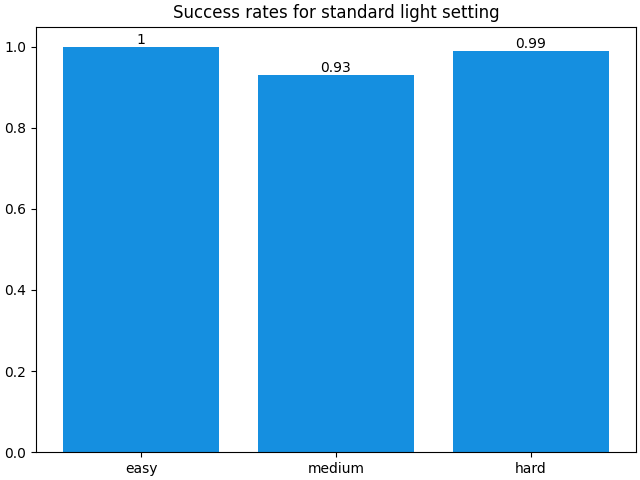
\includegraphics[width=0.45\textwidth]{Bilder/notebook_images/hardDistanceStandardLight_eval_standard_success_rates_barplot.png}
    \includegraphics[width=0.45\textwidth]{Bilder/notebook_images/hardDistanceStandardLight_eval_standard_collision_rates_barplot.png}
    \caption{Success and collision rates for all difficulties for an agent trained exclusively on hard tracks with standard light}
    \label{fig:hardDistance_generalization}
\end{figure}

\paragraph{Generalization to different light settings}
\label{cha:experiment_fixed_difficulty_light_settings}
Further evaluation of these agents on different light settings showed that the agents were able to generalize to the different light settings as well. The agents were trained on the standard light setting only. However the agents were able to solve episodes with the bright and dark light settings with only slight decreases in performance. The success rates for the different light settings are shown in figure \ref{fig:hardDistance_generalization_light_settings}.

\begin{figure}
    \centering
    \includegraphics[width=0.45\textwidth]{Bilder/notebook_images/hardDistanceStandardLight_eval_all_success_rates_barplot.png}
    \includegraphics[width=0.45\textwidth]{Bilder/notebook_images/hardDistanceStandardLight_eval_all_collision_rates_barplot.png}
    \caption{All success and collision rates for an agent trained exclusively on hard tracks with standard light}
    \label{fig:hardDistance_generalization_light_settings}
\end{figure}

\section{Experiments training with mixed difficulty setting}
\label{cha:experiment_mixed_difficulty}

The next step was to train the agent on all difficulty levels at the same time. The goal was to find hyperparameters that would allow the agent to learn to solve all difficulty levels better than with the previous exclusive training. The agent was trained on all difficulty levels at the same time with the same hyperparameters that were used before. The $trainingMapType$ parameter was set to $randomEval$, this results in split of 20\% easy, 40\% medium and 40\% hard tracks.

The training with mixed tracks for the data collection episodes failed. The agent was not able to learn to solve the tracks as successfully as the isolated training on hard tracks. Further changes to the hyperparameters did not improve the learning process. For example the amount of data collected in each iteration was increased to balance out the increased variety of tracks.

% put a figure here? or in the appendix?

\section{Experiments training with mixed light setting hyperparameter}
\label{cha:experiment_mixed_light}

In the previous experiments, the complexity of the task was reduced by focussing on single light settings. The goal was to test the parameters and find configurations that enable the agent to learn the tasks with increasing complexity. The experiments showed that an agent that is trained on hard tracks exclusively is able to generalize to the lower difficulty tracks as well. These agents were also able to solve the tracks of differenct light settings with only slight differences in performance.


The next step was to train the agent on all light settings at the same time. The goal was to find hyperparameters that would allow the agent to learn to solve the tracks with different light settings better than with the previous exclusive training. The agent was trained on difficult tracks with all light settings. The $lightSetting$ parameter was set to $random$, this results in split of 33\% bright, 33\% standard and 33\% dark illumination for the data collection episodes.

\paragraph{Resuts for standard light setting}

The agent was able to learn to solve the tracks of different difficulties. Similarly to the previous experiments, the agent was able to generalize to the easy and medium tracks. The agent was able to solve the easy, medium and hard tracks with success rates of 100\%, 100\% and 99\% \ref{fig:hardDistance_mixedLight_generalization}. 

This is an improvement over the agent trained exclusively on hard tracks with standard light \ref{cha:experiment_fixed_difficulty}.
This improvement may be due to the increased variety of data encountered during the training phase.

\begin{figure}
    \centering
    \includegraphics[width=0.45\textwidth]{Bilder/notebook_images/hardDistanceMixedLight_eval_standard_success_rates_barplot.png}
    \includegraphics[width=0.45\textwidth]{Bilder/notebook_images/hardDistanceMixedLight_eval_standard_collision_rates_barplot.png}
    \caption{Success and collision rates for all difficulties with standard light for an agent trained on hard tracks with all light settings}
    \label{fig:hardDistance_mixedLight_generalization}
\end{figure}

\paragraph{Performance on all light settings}

The agent was evaluated on the different light settings. The agent was able to solve the episodes reliably for all light settings. There were only slight differences in performance between the light settings for hard tracks \ref{fig:hardDistance_mixedLightTraining_results}.


The agent performed much better in episodes with bright or dark light setting compared to the agent trained exclusively on tracks with standard light \ref{cha:experiment_fixed_difficulty}. This was to be expected as the agent was trained on all light settings.

\begin{figure}
    \centering
    \includegraphics[width=0.45\textwidth]{Bilder/notebook_images/hardDistanceMixedLight_eval_all_success_rates_barplot.png}
    \includegraphics[width=0.45\textwidth]{Bilder/notebook_images/hardDistanceMixedLight_eval_all_collision_rates_barplot.png}
    \caption{Success and collision rates for an agent trained on hard tracks with all light settings}
    \label{fig:hardDistance_mixedLightTraining_results}
\end{figure}



\section{Experiments on the importance of the histogram equalization preprocessing step}

The previous training results showed that the agent was able to learn to solve the tracks with different light settings. The agents used the histogram equalization preprocessing step \ref{sec:histogram_equalization} to increase the resiliency towards light changes. Agents that were trained on the standard light setting were able to solve tracks under bright and dark light conditions as well. This implies the histogram equalization plays a big role.

\paragraph{Evaluating an agent without the histogram equalization preprocessing step}

The agent from the previous section about mixed light settings during training was evaluated without the histogram equalization preprocessing step. This agent was trained with the histogram equalization step. The removal of the preprocessing step leads to a performance collapse for the standard and dark settings \ref{fig:hardDistance_mixedLight_comparison_withWithoutHistogramEqualization}. The success rate drops to 0\% for the dark light setting.
The performance for the bright light setting is not affected as severely. Nevertheless the success rate drops from 98\% to 62\% for the hard tracks.

The decrease in performance was to be expected, as the agent was trained with the histogram equalization preprocessing step. The histogram equalization step changes the image content substantially \ref{table:preprocessing_steps}. The agent has learned to use the output of the preprocessing step. As a result, the agent is not able to solve the tracks without the preprocessing step.

\begin{figure}
    \centering
    \subfigure[Success rate with histogram equalization]{\includegraphics[width=0.45\textwidth]{Bilder/notebook_images/hardDistanceMixedLight_eval_all_success_rates_barplot.png}}
    \subfigure[Success rate without histogram equalization]{\includegraphics[width=0.45\textwidth]{Bilder/notebook_images/hardDistanceMixedLight_evalWithoutHistEqualization_all_success_rates_barplot.png}}
    \caption{Success rates for an agent trained on all light settings with histogram equalization}
    \label{fig:hardDistance_mixedLight_comparison_withWithoutHistogramEqualization}
\end{figure}


\paragraph{Training an agent without the histogram equalization preprocessing step}
An agent without the histogram equalization preprocessing step was trained on the mixed light setting to determine if the preprocessing step is required for high performance. The results of training an agent without the preprocessing step are shown in the second graph in \ref{fig:hardDistance_mixedLight_noHistogramEqualizationTraining_results}. The agent was not able to learn to solve the hard tracks as successfully as the agent trained with the histogram equalization preprocessing step. The difference is noticeable but quite small at 2\% for the success rate of hard tracks.

\begin{figure}
    \centering
    \subfigure[Agent trained with histogram equalization]{\includegraphics[width=0.45\textwidth]{Bilder/notebook_images/hardDistanceMixedLight_eval_all_success_rates_barplot.png}}
    \subfigure[Agent trained without histogram equalization]{\includegraphics[width=0.45\textwidth]{Bilder/notebook_images/hardDistanceMixedLight_noHistEqualization_all_success_rates_barplot.png}}
    \caption{Success rate comparison for an agent that is trained with or without histogram equalization on all light settings}
    \label{fig:hardDistance_mixedLight_noHistogramEqualizationTraining_results}
\end{figure}

\paragraph{Conclusion}
The histogram equalization step contributes strongly to the resiliency to light changes for the constructed agent. It is possible to train a resilient agent without the histogram equalization preprocessing step.
However the best performance is achieved when the agent is trained with the histogram equalization preprocessing step and all light settings.

The histogrm equalization preprocessing step should never be removed or added after the training is complete, this results in a performance decrease.

\section{Comment on the collision rate}

The trained agents are able to complete the parcours very reliably. However the agents do not avoid collisions entirely. The collision rate generally increases for higher difficulty tracks. The collision rates vary quite strongly between the different trained models. The agent trained on the mixed light setting has a collision rate of 70\% for the hard tracks with standard light setting \ref{fig:hardDistance_mixedLightTraining_results}. Whereas the agent trained on hard tracks with standard light setting has a collision rate of only 29\% \ref{fig:hardDistance_generalization}.

The agents are able to complete the tracks reliably despite the collisions. The analysis of successful episodes with collisions shows that these collisions are only minor collisions. The agent collides with the goal obstacles at its side. The agent basically scapes against the goal posts. The agent does not collide with the goal obstacles head on \ref{fig:example_collision}.

\begin{figure}
    \centering
    \includegraphics[width=0.45\textwidth]{Bilder/example_minor_collision_topview_frame_1295.png}
    \caption{Example of a collision from a successfully completed episode}
    \label{fig:example_collision}
\end{figure}

The reason for the high collision rates is the selected reward function. The agents were trained with the distance reward function exclusively following the first experimentations. The distance reward function does not penalise collisions directly. The distance reward function only discourages collisions indirectly. Collisions that prevent an agent from moving towards the next goal result in less collected reward. For example a frontal collision of the agent with a goal post object requires the agent to then move backwards and around the goal post. The backwards movement is penalized. The agent learns to avoid frontal collisions.

The minor collisions that occur are not penalized as the agent is still able to move towards the next goal. As a result the agent does not learn to avoid these collisions entirely.


\section{Hard Tracks, mixed light settings - the most successful policy}
\label{sec:most_successful_policy}

This section summarizes how the most successful policy was implemented and trained. The parameters were chosen following the previous experiments. This policy is used for the evaluations of the three main research goals.
The policy was trained using the distance reward alone. It was trained on hard tracks with all light settings. The policy used the histogram equalization preprocessing step.

\paragraph{Policy Settings}
The policy was configured to use the three preprocessing steps downsampling, greyscaling and histogram equalization. The policy used a frame stacking of 10. The agent camera image had a resolution of $500x168$ which was downsampled to $250x84$. This results in an observation space of shape $[84, 250, 10]$. The duration of steps was fixed to $0.3$ seconds.
The neural network follows the earlier descriptions exactly \ref{sec:network_architecture}. It consisted of a feature extractor part with 3 convolutional layers and one fully connected layer. The feature extractor takes the observation as input, its outputs are used by the action and value head. The action and value head each consist of a single fully connected layer. The entire network is trained together end-to-end using backpropagation of the loss defined by the PPO algorithm.

\paragraph{Reward function}
The policy was trained exclusively using the distance reward. The other reward functions were not used \ref{fig:final_reward_function}.

\paragraph{Training data}
The episodes for data collection used hard tracks with all light settings. The agent was initialized with random orientations. The episodes were not reset upon collision.

\paragraph{Training algorithm settings}
The training was configured to use 10 environments in parallel to collect data. 2560 samples were collected in each data collection step. The training was terminated after a total of 2385920 steps. 8423 full episodes were executed to collect these samples. 233 data collection and model training iterations were executed in total. The total training duration was 1.02 days.
The training progress can be seen in figure \ref{fig:training_most_successful_model}. The model reached a success rate of 100\% for the collected episodes.


The full training config can be found in the appendix \ref{cha:most_successful_config}.

\begin{figure}
    \centering
    \subfigure[Distance Reward]{\includegraphics[width=0.3\textwidth]{Bilder/tensorboard_images/successfulTraining_distance_reward.png}}
    \subfigure[Goal completion rate]{\includegraphics[width=0.3\textwidth]{Bilder/tensorboard_images/successfulTraining_goal_completion_rate.png}}
    \subfigure[Success rate]{\includegraphics[width=0.3\textwidth]{Bilder/tensorboard_images/successfulTraining_success_rate.png}}
    \caption{Properties of the collected episodes over time for the most successful model}
    \label{fig:training_most_successful_model}
\end{figure}

%%\chapter{Methods}
%\label{cha:Methods}
%\lipsum \autocite{DBLP:books/sp/HarderR01}

\section{Investigating the feasibility of transfering the policy to a physical robot.}

Previous sections describe how a policy was developed that can be used to control an agent in a simulated environment. This section describes how I will investigate the feasibility of transfering the developed policy onto physical devices. The simulated agent was modeled after a Nvidia JetBot. The Nvidia JetBot is a small robot that is equipped with a camera, a processing unit and two motors that can be controlled independently. 
The Nvidia Jetbot is designed to be able to execute AI software. However the limited computational power of the JetBot raises the question whether the developed policy can be transfered to the JetBot. 

The developed policy takes a camera image from the front of the agent as input and applies preprocessing steps to the image. The preprocessed image is then processed by a convolutional neural network that outputs two acceleration values, one for each motor. The acceleration values are applied to the motors for a fixed amount of time. While the agent is moving, the camera image is constantly updated and the policy is applied to the new image. It is crucial that the agent's policy can be computed quick enough to be able act in real time. 

\subsection{effects of insufficiently slow policy computation}
If the jetbot is not able to compute the developed policy in the required time, there are two options that do not require changes to the developed/trained policy. The first option is to stop the motors until the policy is computed and then apply the acceleration values. This would make the jetbot movement overall slower and less smooth.
The second option is to apply the last computed acceleration values to the motors until the new policy is computed. This could result in a degradation of the jetbot's performance since the actions would be less accurate.
The two options are shown with visual representations in \ref{fig:slow_policy_computation}.


% gif splitter
% https://ezgif.com/split



\newcommand{\spc}[2]{\subfigure[#1]{\includegraphics[width=0.2\textwidth]{Bilder/slow_policy_computation/#2.png}}}
%\newcommand{\spc}[2]{\begin{subfigure}{.5\textwidth}\centering\includegraphics[width=0.2\textwidth]{Bilder/slow_policy_computation/#2.png}\caption*{#1}\end{subfigure}}
% trying to remove a), b) ... https://tex.stackexchange.com/questions/165508/remove-a-b-from-subfigure-numbering-but-keep-the-subfigure-caption

\begin{figure}
    
    \begin{center}
    \begin{tabular}{|| c | c | c ||} 
        \hline
        Policy computation in time & \makecell{Option 1: \\ Wait} & \makecell{Option 2:\\ Apply previous outputs}  \\ [0.5ex] 
        \hline\hline
        \spc{Start}{start} &  \spc{Start}{start} & \spc{Start}{start} \\ 
        \hline
        \spc{Agent turns right}{agent_turns_right} & \spc{Agent turns right}{agent_turns_right} & \spc{Agent turns right}{agent_turns_right} \\
        \hline
        \spc{Agent stops turning and goes strait}{agent_turns_left} & \spc{Agent waits}{agent_turns_right} & \spc{Agent continues to turn}{agent_fails_to_turn_left} \\
        \hline
        \spc{Agent continues}{agent_continues_properly}  & \spc{Agent stops turning and goes strait}{agent_turns_left} & \spc{Agent crashes}{agent_crashes} \\
        \hline
        \makecell{Agent moves properly.}  & \makecell{Agent overall speed is reduced.} & \makecell{Agent behaviour is changed.} \\
        \hline
    \end{tabular}
    \end{center}
    \caption{Effects of slow policy computation on the performance.}
    \label{fig:slow_policy_computation}
\end{figure}






\chapter{Challenges}
\label{cha:challenges}

\section{Connecting the Python algorithm and Unity Simulation}

The first challenge was to connect the Python algorithm with the Unity simulation. The Python algorithm is responsible for training the agent, while the Unity simulation is responsible for rendering the environment and providing the agent with observations and rewards. The environment is wrapped in a gymnasium environment \autocite{gymnasium}, this way it can be integrated with many existing reinforcement learning libraries and algorithms. The unity simulation acts as a JsonRPC server, the python gymnasium environment acts as a client. 

\paragraph{Data exchange}
The first challenge was to transfer the image data from unity to python. This was solved by encoding the image data as a base64 string and sending it back to python over the network. The image data was then decoded in python and converted to a numpy array.

\paragraph{Communication Speed}
The seperation of the simulation and the reinforcement learning algorithm introduces a delay for all interactions with the simulated environments. This is most noticeable in the data collection part of the training loop, since the environment has to execute the actions of the agent and send back the new observations and rewards. 
The reinforcement learning library stable-baselines3 \autocite{sb3} was used for the training of the agent. This library is built to enable the parallel execution of multiple environments. However the library requires that actions are performed on all environments at the same time. Together with the delay caused by communication, this parallel execution would slow down significantly.

The solution to this problem was bundling the actions for the different environments and sending them to unity in one batch. The unity server then executes the actions on the individual environments. This way the delay caused by the communication overhead is only introduced once per batch of actions.

\section{step duration}
non blocking steps

TODO explain that a fixed step duration makes the policy transferable to other devices (eval runs with fixed step duration should have the same result for a particular trained policy)

\section{Parameters for training}

journey to the good parameters in ExperimentsTrainingParameters.tex

\chapter{Results}
\label{cha:Results}

This chapter presents the results of the experiments conducted in this project. The first three experiments were designed to answer the research questions posed in chapter \ref{cha:ResearchGoals} specifically. 

The experiments were conducted using the policy that was developed as a result of the parameter experimentation \ref{sec:most_successful_policy}. This policy was trained exclusively on hard tracks with all light settings. The histogram equalization preprocessing step was used during training.


\section{Eval for question 1 - \questionOne}

The trained policy was evaluated on tracks of all difficulty settings with the standard light setting using the Basic Evaluation algorithm \ref{sec:basic_evaluation_algorithm} with 100 episodes per setting. The success rates for the different difficulty settings are shown in figure \ref{fig:result_success_rates_standard}. Example videos of the agent's behaviour during evaluation can be found in the appendix \ref{cha:example_videos}.

\subsection{Experiment Results}

\begin{figure}
    \centering
    \includegraphics[width=0.45\textwidth]{Bilder/notebook_images/hardDistanceMixedLight_eval_standard_success_rates_barplot.png}
    \includegraphics[width=0.45\textwidth]{Bilder/notebook_images/hardDistanceMixedLight_eval_standard_collision_rates_barplot.png}
    \caption{Success and collision rates for standard light setting.}
    \label{fig:result_success_rates_standard}
\end{figure}


The policy completed the easy, medium and hard tracks with a succes\_rate of 100\%, 100\% and 99\%. 
The collision\_rates were 0\%, 1\% and  70\%. Especially for the hard difficulty setting, the agent does not avoid collisions completely. 

The analysis of successful episodes with collisions shows that these collisions are only minor collisions. The agent passes the goals very close to the goal post that is closer to the arena middle \ref{fig:agent_behaviour}. This often results in collisions with the goal obstacles at its side.

\begin{figure}
    \centering
    \subfigure[Agent passes the goal close to the arena middle]{\includegraphics[width=0.45\textwidth]{Bilder/example_goal_passing_close_to_middle.png}}
    \subfigure[Agent may collide with goal post at the side]{\includegraphics[width=0.45\textwidth]{Bilder/example_minor_collision_topview_frame_1295.png}}
    \caption{Goal passing behaviour of the trained agent}
    \label{fig:agent_behaviour}
\end{figure}

The unsuccessful episodes of hard tracks were analysed to determine why the agent does not reach 100\% success rates. The analysis showed that the agent has frontal collisions with the first goal post at the agents side \ref{fig:unsuccessful_episodes}. This occurs only when the agent is spawned with an extreme rotation. The agent cannot complete the tracks in about 40\% of episodes with the maximum rotation of $15^{\circ}$.

\begin{figure}
    \centering
    \subfigure[Agent is spawned with extreme rotation]{\includegraphics[width=0.3\textwidth]{Bilder/extremeSpawnRot_agent_initial.png}}
    \subfigure[Agent approaches first goal post]{\includegraphics[width=0.3\textwidth]{Bilder/extremeSpawnRot_agent_turns.png}}
    \subfigure[Agent collides with first goal post and remains stuck]{\includegraphics[width=0.3\textwidth]{Bilder/extremeSpawnRot_agent_collides.png}}
    \caption{Analysis of unsuccessful episodes}
    \label{fig:unsuccessful_episodes}
\end{figure}



\subsection{Conclusion}

The trained policy is able to complete all difficulty levels very reliably. The policy reached success rates of 100\%, 100\% and 99\% for easy, medium and hard tracks. The end-to-end trained \ac{CNN} policy proves to be very effective at solving the autonomous driving task.

The policy outperforms previous work at the ScaDS.AI by \textcite{maximilian}. The policies developed by \textcite{maximilian} reached success rates of 99\%, 89\% and 64\% for easy, medium and hard tracks.

The policy was trained on the difficult setting only. The policy did not see easy and medium difficulty tracks before the evaluation. The policy is able to generalize to tracks of lower difficulty.

\section{Eval for Question 2 - \questionTwo}

The most succesfull model was used to evaluate the agent's performance under different light settings. The agent was evaluated on the standard, dark and bright light settings. Each combination of difficulty and light setting was evaluated with the Basic Evaluation Algorithm for 100 episodes. The success rates for the different light settings are shown in figure \ref{fig:result_success_rates_lightSettings}.


\subsection{Experiment Results}

\begin{figure}
    \centering
    \includegraphics[width=0.45\textwidth]{Bilder/notebook_images/hardDistanceMixedLight_eval_all_success_rates_barplot.png}
    \includegraphics[width=0.45\textwidth]{Bilder/notebook_images/hardDistanceMixedLight_eval_all_collision_rates_barplot.png}
    \caption{Success and collision rate comparisons for light settings.}
    \label{fig:result_success_rates_lightSettings}
\end{figure}

The success rates for all light and difficulty settings are very high at above 95\%. The agent completed the easy and medium tracks with a success rate of 100\%. The light setting had no influence on the success\_rate for the easy and medium tracks.
The evaluations for the bright and dark light settings show slight decreases in performance compared to the standard light setting for hard tracks. The success\_rate of hard tracks in the bright and dark light setting was 98\% and 97\%.

The collision rates are very low for the easy and medium tracks. All tracks in these settings were solved without collisions except for the medium tracks with the standard light setting. This medium standard evaluation had a collision rate of 1\%.
The collision rates for the hard tracks are quite high at 70\% for the standard light setting. The bright and dark light settings are very high as well with 70\% and 62\%.

Across all light and difficulty settings the overall success rate is almost 100\% and the overall collision rate is 22\%.

\subsection{Conclusion}

The policy was able to complete the tracks very reliably under the different light settings. The light setting only had a minor impact on the success rate.
Furthermore the different light settings did not lead to an overall increase in collisions.

The developed policy was trained following the experiments in the previous chapter. The agent used the histogram equalization preprocessing step and mixed light settings during training. Using these settings the policy was able to learn to navigate the tracks with all light conditions.


\section{Eval for Question 3 - \questionThree}

The most successful model was used to record replays of the agent's behaviour. This most successful model used a $fixedTimestepLength$ of $0.3$ seconds. This means the hardware has to able to make a decision every $0.3$ seconds to be considered fast enough.

Five episodes were recorded for each difficulty and light setting combination. As expected from the previous evaluations of the policy, the replay episodes had a very high success\_rate of 100\%. The recorded episodes were then replayed on the Nvidia Jetbot. The time it took to replay the episodes was measured \ref{fig:result_replay_times}. The policy outputs from the replay were compared to the policy outputs from the recordings \ref{fig:result_replay_outputs}. The differences are caused by the hardware and software differences between the training and the replay environment.


\begin{figure}
    \centering
    \includegraphics[width=0.5\textwidth]{Bilder/notebook_images/replay_times.png}
    \caption{Replay times on jetbot hardware}
    \label{fig:result_replay_times}
\end{figure} % a chart showing the replay times (max, min, mean)


\begin{figure}
    \centering
    \includegraphics[width=0.45\textwidth]{Bilder/notebook_images/replay_outputs_action_left.png}
    \includegraphics[width=0.45\textwidth]{Bilder/notebook_images/replay_outputs_action_right.png}
    \caption{Differences in policy outputs between recordings and replays on jetbot hardware}
    \label{fig:result_replay_outputs}
\end{figure} % a chart showing the replay outputs


\subsection{Experiment Results}

\paragraph{Replay times}

The replay times for the recordings on jetbot hardware are shown in figure \ref{fig:result_replay_times}. The maximum duration was $0.216$ seconds. The mean is much lower at $0.067$ seconds. The plot shows that the maximum duration was an extreme outlier.
Given the $fixedTimestepLength$ of $0.3$ seconds and the maximum duration of $0.216$ seconds, the hardware is fast enough to replay the episodes. This leaves at least $0.084$ seconds for the agent to receive an image from the camera and send the new instruction to the motors.

The cameras used in the nvida jetbot are capable of capturing images with a resolution of $1280x720$ pixels at $60$ frames per second. This means the camera can capture an image every $0.0166$ seconds. The hardware is quick enough to compute actions in real time.

% times replay hardDistanceMixedLight: min 0.06319522857666016, mean 0.06662133265668013, max 0.21592259407043457

\paragraph{Policy Outputs}

The policy outputs from the recordings and the replays on jetbot hardware are nearly identical. The differences are shown in figure \ref{fig:result_replay_outputs}. The outputs were reproduced very closely. The maximum difference was $4.69e-03$.  This is difference is negligeable compared to the range of policy outputs $[-1,1]$.

% left action differences min [0.], max [0.00433731], mean 0.00030147546203806996, std 0.0004885991802439094
% right action differences min [0.], max [0.00468674], mean 0.00030857478850521147, std 0.000496754830237478

\subsection{Discussion}

The jetbot hardware is capable enough to compute the policy in real time. The differences of the policy outputs between the recordings and the replays are very small, the policy outputs were reproduced very closely. This suggests the differences in hardware and software do not impact the policy significantly.

\section{Other Experiments}

\subsection{Sampling Mode Performance Test}
\label{ref:sampling_mode_test_results}

The sampling mode performance test uses the Basic evaluation algorithm to evaluate an agent with derministic and non-deterministic sampling for each difficulty level. The success rates for the two sampling modes are compared to determine if the agent's performance is influenced by the sampling method. The sampling mode test was executed for all agents during the experimentation phase of this project using standard light.

\paragraph{Results}
The tests showed that the difference in performance for the sampling modes was very small for the trained policies. The results showed empirically that non-deterministic sampling leads to better success rates. Nevertheless some policies performed slightly worse using the non-deterministic sampling mode. The success rate was on average 1.7\% higher when using non-deterministic sampling. The biggest difference was 2.6\% for the medium difficulty setting \ref{fig:deterministic_check_result}.

\begin{figure}
    \centering
    \includegraphics[width=0.8\textwidth]{Bilder/notebook_images/deterministic_check_results.png}
    \caption{Results of the deterministic check across all evaluations during the experimentation phase}
    \label{fig:deterministic_check_result}
\end{figure}

\paragraph{Discussion}
The test indicates that the non-deterministic sampling mode performes better, although the differences in performance are quite small. Given these results, the main evaluations for question 1 and 2 were conducted with non-deterministic sampling.

\subsection{Identical Start Condition Test}

The environment is not 100\% deterministic. This is due to the environment implementation in Unity \autocite{unity_fixed-update}. The environment uses physics simulations which are not fully deterministic. In addition the policy's actions are sampled non-deterministically during the evaluation.
This means that identical start conditions of an episode may result in different trajectories and results. This test evaluates the impact of the non-deterministic environment and sampling on the agent's behaviour. 

The agent with \ac{HX-P} is placed in the same start conditions for 100 episodes. The starting conditions entail the selected track, light condition and the agent's starting rotation. The test was executed for the hardBlueFirstRight trach with the standard lighting. Three starting rotations were used \ref{fig:identical_start_conditions_test_rotations}.
The episode results are compared.

\begin{figure}
    \centering
    \subfigure[-15°]{\includegraphics[width=0.3\textwidth]{Bilder/image_printer_images/identical_start_conditions/hardBlueFirstRight_minus15.png}}
    \subfigure[0°]{\includegraphics[width=0.3\textwidth]{Bilder/image_printer_images/identical_start_conditions/hardBlueFirstRight_0.png}}
    \subfigure[15°]{\includegraphics[width=0.3\textwidth]{Bilder/image_printer_images/identical_start_conditions/hardBlueFirstRight_15.png}}
    \caption{tested starting rotations}
    \label{fig:identical_start_conditions_test_rotations}
\end{figure}

\paragraph{Results}

The results show that the policies's performance is very consistent for the different starting rotations regarding the $success\_rate$. The agent successfully completes the tracks with $-15°$ and $0°$ starting rotation. The agent completes the track in only 7\% of episodes with $15°$ starting rotation.
For the different starting rotations, the agent either completes the track very reliably or very rarely.

The $collision\_rate$ is not consistent for the episodes with the same starting rotation. The $collision\_rate$ is 60\% and 72\% for the $-15°$ and $0°$ starting rotations. 

\begin{figure}
    \centering
    \includegraphics[width=0.8\textwidth]{Bilder/notebook_images/identicalResults_mixedLightSettings.png}
    \caption{Results of 100 episodes for different starting rotations}
    \label{fig:identical_start_conditions_test_result}
\end{figure}


\paragraph{Discussion}

The test shows that identical starting conditions do not always lead to the same episode result. However the success rate is very consistent for the identical starting conditions. The collision rate is significantly less consistent.

The results confirm that the $success\_rates$ of the Basic Evaluation Algorithm are reliable. 


\subsection{Fresh Observations Test}

\ac{HX-P} was trained to not use fresh observations with a fixed step duration of 0.3 seconds. The policy input receives the observation from the start of the previous step as input. The policy input essentially lags 0.3 seconds behind the environment state. This saves processing time during training and evaluation. Alternatively a policy can be run with the $use\_fresh\_obs$ parameter. This makes the policy request a fresh observation from the Unity simulation, see \ref{sec:non_blocking_step_calls}.

The Fresh Observations Test analyses whether switching the trained policy to use fresh observations improves the performance. The policy is evaluated with fresh observations and without fresh observations for each difficulty level using the Basic Evaluation Algorithm \ref{sec:basic_evaluation_algorithm}. The success rates are compared to determine if fresh observations improve the agent's performance.

\paragraph{Results}

\begin{figure}
    \centering
    \includegraphics[width=0.8\textwidth]{Bilder/notebook_images/hardDistanceMixedLight_eval_freshNonFresh_success_rates_barplot.png}
    \caption{Success rates for \ac{HX-P} using fresh and non-fresh observations}
    \label{fig:fresh_observations_test_result}
\end{figure}

The results show that the policy performs similar for the easy and medium settings. The success rates are 100\% for both fresh and non-fresh observations. The hard setting shows a strong decrease in performance when using fresh observations. The success rate drops from 98\% to 68\% \ref{fig:fresh_observations_test_result}.

The evaluations using fresh observations also take longer. The Basic Evaluation Algorithm's per call time for the fresh observations is about 20 minutes compared to 17 minutes for the non-fresh observations. The evaluation using fresh observations is slower because the policy has to request a fresh observation from the Unity simulation. This takes additional time.


\paragraph{Discussion}

The policy was trained using non-fresh observations. The policy's performance decreases for hard tracks when it is evaluated using fresh observations.
This suggests that the policy has learned to work with the lag of 0.3 seconds between the environment state and input to the policy. The policy's performance decreases when the lag is removed.

The test confirms that the $use\_fresh\_obs$ parameter should not be changed after the training has been completed.


\subsection{Jetbot Generalization Test}

\ac{HX-P} was trained using the DifferentialJetBot shown in figure \ref{fig:jetbots}. The Jetbot Generalization test evaluates the same policy using the FourWheelJetBot. The policy is only evaluated on the standard light setting to save time.

\paragraph{Results}

\begin{figure}
    \centering
    \includegraphics[width=0.45\textwidth]{Bilder/notebook_images/hardDistanceMixedLight_eval_jetbot_generalization_success_rates_barplot.png}
    \includegraphics[width=0.45\textwidth]{Bilder/notebook_images/hardDistanceMixedLight_eval_jetbot_generalization_collision_rates_barplot.png}
    \caption{Evaluation of the DifferentialJetBot policy \ac{HX-P} with both jetbot versions}
    \label{fig:result_jetbot_generalization}
\end{figure} % a chart showing the replay outputs

The policy evaluation achieves very high success rates for the FourWheelJetBot with 100\%, 100\% and 91\% for the easy, medium and hard tracks \ref{fig:result_jetbot_generalization}. The collision rates increase for higher difficulties with 0\%, 4\% and 94\%. 
The success and collision rates are slightly worse than on the DifferentialJetBot. The overall success rate of the FourWheelJetBot is 97\% compared to 100\% for the DifferentialJetBot. 

The overall collision rate is 33\% compared to 24\% for the DifferentialJetBot. Especially for the hard tracks the collision rate is much higher for the FourWheelJetBot with 94\% compared to 70\% for the DifferentialJetBot.
The collisions of the DifferentialJetBot were previously described as mainly being minor collisions where the agent scrapes the goal posts with its side. Analysis of the recorded videos shows that the collisions of the FourWheelJetBot are similar. However the agent scrapes the goals on its side for longer durations \ref{sec:fourwheel_collisions}.

% strong collisions here: hard_standard_FourWheelJetBot_env_0_video_2_topview

\paragraph{Discussion}

The policy that was trained on the DifferentialJetBot can be transfered to the FourWheelJetBot with only a slight decrease in performance.
The policy does not have to be retrained in this case. 



\chapter{Conclusion}
\label{cha:Conclusion}

bla conclusion



% Literaturverzeichnis -----------------------------------------------------
%		Das Literaturverzeichnis wird aus der Datenbank erstellt.
%		Die genaue Verwendung von biblatex wird hier jedoch nicht erklärt.
%		Links: 	https://ctan.org/pkg/biblatex?lang=de
%						https://de.overleaf.com/learn/latex/Articles/Getting_started_with_BibLaTeX
% --------------------------------------------------------------------------


% Mit Overleaf compilieren, falls es Probleme gibt mit der Bibliographie

\printbibliography


% \setcounter{page}{122}
% \pagenumbering{gobble}
%\pagenumbering{gobble}
\addchap{Erklärung}
Ich versichere, dass ich die vorliegende Arbeit mit dem Thema:

\begin{center}
\textit{\glqq\titel\grqq}\\[1em]
\end{center}
			
selbständig und nur unter Verwendung der angegebenen Quellen und Hilfsmittel angefertigt habe, insbesondere sind wörtliche oder sinngemäße Zitate als solche gekennzeichnet. Mir ist bekannt, dass Zuwiderhandlung auch nachträglich zur Aberkennung des Abschlusses führen kann. Ich versichere, dass das elektronische Exemplar mit den gedruckten Exemplaren übereinstimmt.
\par
\ort, den \eingereicht


\rule[-0.2cm]{5cm}{0.5pt}

\textsc{\autor} 
	% Selbständigkeitserklärung 

% Anhang -------------------------------------------------------------------
%		Die Inhalte des Anhangs werden analog zu den Kapiteln inkludiert.
%		Dies geschieht in der Datei Anhang.tex
% --------------------------------------------------------------------------
\appendix
\clearpage
\renewcommand*{\thesection}{\Alph{section}}
\pagenumbering{Roman}

\chapter{Appendix}
\label{cha:Appendix}

\section{Code Repository}

The code repository is publically availible on GitHub: 
\href{https://github.com/geschnee/carsim-rl-cnn}{carsim-rl-cnn}

The readme file contains instructions on how to install and run the code.

\section{Most successful model}

The most successful model is publically availible on Huggingface: 
\href{https://huggingface.co/geschnee/carsim-rl-cnn}{carsim-rl-cnn}

\href{https://huggingface.co/geschnee/carsim-rl-cnn/blob/main/models/hardDistanceMixedLight.zip}{hardDistanceMixedLight.zip}

The episode recordings for question 3 are also hosted there.


\subsection{Most Successful Policy Configuration}
\label{cha:most_successful_config}

The training config of the model for the final evaluations is availible on GitHub: 
\href{https://github.com/geschnee/carsim-rl-cnn/tree/main/python/cfg/hardDistanceMixedLight.yaml}{hardDistanceMixedLight.yaml}

\section{Example Video Files}
\label{cha:example_videos}

Video Files are availible on Github: 
\href{https://github.com/geschnee/carsim-rl-cnn/tree/main/python/results/example_videos}{example\_videos}

\subsection{Video Files with FourWheelJetBot}

\paragraph{Collisions}
\label{sec:fourwheel_collisions}

\href{https://huggingface.co/geschnee/carsim-rl-cnn/blob/main/example_videos_FourWheelJetbot/hard_standard_FourWheelJetBot_env_0_video_1_topview.gif}{example\_videos/hard\_standard\_FourWheelJetBot\_env\_0\_video\_1\_topview.gif}
\href{https://huggingface.co/geschnee/carsim-rl-cnn/blob/main/example_videos_FourWheelJetbot/hard_standard_FourWheelJetBot_env_0_video_2_topview.gif}{example\_videos/hard\_standard\_FourWheelJetBot\_env\_0\_video\_2\_topview.gif}

% z.B. Pseudocode



\section{Experiments for finding hyperparameters}

\subsection{Reward functions capability check}
The used configs are the following:
\begin{itemize}
    \item \href{https://github.com/geschnee/carsim-rl-cnn/tree/main/python/cfg/ppo_rewardFunction_capability_check_orientationReward.yaml}{ppo\_rewardFunction\_capability\_check\_orientationReward.yaml}
    \item \href{https://github.com/geschnee/carsim-rl-cnn/tree/main/python/cfg/ppo_rewardFunction_capability_check_distanceReward.yaml}{ppo\_rewardFunction\_capability\_check\_distanceReward.yaml}
    \item \href{https://github.com/geschnee/carsim-rl-cnn/tree/main/python/cfg/ppo_rewardFunction_capability_check_velocityReward.yaml}{ppo\_rewardFunction\_capability\_check\_velocityReward.yaml}
    \item \href{https://github.com/geschnee/carsim-rl-cnn/tree/main/python/cfg/ppo_rewardFunction_capability_check_eventReward.yaml}{ppo\_rewardFunction\_capability\_check\_eventReward.yaml}
\end{itemize}



\section{Pseudocode}

TODO pseudocde für eval\_model\_track?

\renewcommand{\thepseudonum}{\roman{pseudonum}}
\begin{pseudocode}{Collect Data}{ }
\COMMENT{Fill RolloutBuffer with samples obtained by current model}\\

\PROCEDURE{CollectData}{trainingMapType, trainingLightSetting}
num\_steps \GETS 0\\
num\_episodes \GETS 0\\
num\_succesful\_episodes \GETS 0\\

RolloutBuffer.\CALL{Reset}{trainingMapType, trainingLightSetting}\\
Env.\CALL{Reset}{}\\
\WHILE RolloutBuffer.\CALL{NotFull}{} \DO
\BEGIN
obs \GETS Env.\CALL{GetObservation}{}\\
action \GETS Model.\CALL{GetAction}{obs}\\
reward \GETS Env.\CALL{Step}{action}\\
num\_steps \GETS num\_steps + 1\\
\CALL{AddToRolloutBuffer}{obs, action, reward}\\
\IF Env.\CALL{IsFinished}{} \THEN
\BEGIN
num\_episodes \GETS num\_episodes + 1\\
\IF Env.\CALL{FinishedSuccessfully}{} \THEN
\BEGIN
num\_succesful\_episodes \GETS num\_succesful\_episodes + 1\\
\END\\
Env.\CALL{Reset}{trainingMapType, trainingLightSetting}\\
\END\\
\END\\

rollout\_success\_rate \GETS \frac{num\_succesful\_episodes}{num\_episodes}\\

\IF rollout\_success\_rate >= best\_rollout\_success\_rate \THEN
\BEGIN
best\_success\_rate \GETS rollout\_success\_rate\\
Model.\CALL{SaveToFile}{}\\
best\_model \GETS Model\\
\END\\


\RETURN{num\_steps}
\ENDPROCEDURE
\label{pseudocode:collect_data}
\end{pseudocode}

\renewcommand{\thepseudonum}{\roman{pseudonum}}
\begin{pseudocode}{Train Model}{ }
\COMMENT{Sample from replay buffer and update the model based on the loss}\\

\PROCEDURE{TrainModel}{}
amount\_of\_batches \GETS \frac{rollout\_buffer\_size}{batch\_size}\\
\FOR i \GETS 0 \TO n\_epochs \DO
\BEGIN
RolloutBuffer.\CALL{Shuffle}{}\\
RolloutBuffer.\CALL{CreateBatches}{batch\_size}\\
\FOR m \GETS 0 \TO amount\_of\_batches \DO
\BEGIN
batch \GETS RolloutBuffer.\CALL{GetBatch}{m}\\
loss \GETS \CALL{ComputeLoss}{batch}\\
Model.\CALL{Backpropagate}{loss}\\
Optimizer.\CALL{Step}{}\\
\END\\
\END
\ENDPROCEDURE
\label{pseudocode:train_model}
\end{pseudocode}

\section{Neural Network Architecture}

\begin{figure}
    \centering
    \includegraphics[width=0.5\textwidth]{Bilder/action_graph.png}
    \caption{Neural Network Architecture Action Head}
    \label{fig:action_graph}
\end{figure}

\begin{figure}
    \centering
    \includegraphics[width=0.5\textwidth]{Bilder/value_graph.png}
    \caption{Neural Network Architecture Value Head}
    \label{fig:value_graph}
\end{figure}


\section{Eval Model Track}
\renewcommand{\thepseudonum}{\roman{pseudonum}}
\begin{pseudocode}{Generate Map and Rotation Combinations}{ }

\PROCEDURE{generate\_map\_and\_rotations}{difficulty, n\_eval\_episodes, env}

rotationMode \GETS env.\CALL{getSpawnMode}{}\\
rotation\_range\_min, rotation\_range\_max \GETS Spawn.\CALL{getRotationRange}{rotationMode}\\

range\_width \GETS rotation\_range\_max - rotation\_range\_min\\
rotations \GETS []\\

\IF n\_eval\_episodes == 1 \THEN
    rotations.\CALL{append}{(rotation\_range\_min + range\_width)/2}\\
\ELSE
\BEGIN
    step \GETS range\_width / (n\_eval\_episodes -1)\\
    \FOR i \GETS 0 \TO n\_eval\_episodes - 1 \DO
        \BEGIN
        rotations.\CALL{append}{rotation\_range\_min + i * step}\\
        \END\\
\END\\

track\_numbers \GETS MapType.\CALL{getAllTracknumbersOfDifficulty}{difficulty}\\
tracks \GETS []\\
\FOR i \GETS 0 \TO n\_eval\_episodes - 1 \DO
\BEGIN
tracks.\CALL{append}{i \mod \CALL{len}{track\_numbers}}\\
\END\\

combinations \GETS []\\
\FOR i \GETS 0 \TO n\_eval\_episodes - 1 \DO
\BEGIN
combinations.\CALL{append}{(tracks[i], rotations[i])}\\
\END\\

\RETURN{combinations}
\ENDPROCEDURE
\label{fig:generate_track_rotation}
\end{pseudocode}



\section{Replay on JetBot}

\subsection{Installation instructions for executing replays on the Jetbot}

The replays are executed on NVIDIA Jetbot hardware. The test does not make use of jetbot specific hardware and software features such as the jetbot camera. The test runs on the jetbot's standard ubuntu installation. Instructions for the installation and execution of the replay test are availible in the \href{https://github.com/geschnee/carsim-rl-cnn/blob/main/replays_on_jetbot.md}{replays\_on\_jetbot.md file} in the code repository. 


\renewcommand{\thepseudonum}{\roman{pseudonum}}
\begin{pseudocode}{Record Episode}{ }
\COMMENT{Record episode}\\

\PROCEDURE{record\_episode}{policy, env, directory}

env.\CALL{RESET}{}\\

sampled\_actions \GETS [] \\
infer\_obsstrings \GETS [] \\
step\_obsstrings \GETS [] \\

done \GETS \FALSE\\

\WHILE ! done \DO
\BEGIN
obs, obsstring \GETS env.\CALL{GetObservation}{}\\
action \GETS policy.\CALL{Infer}{obs}\\

step\_obsstring, done \GETS env.\CALL{step}{action}\\

infer\_obsstrings.\CALL{append}{obsstring}\\
step\_obsstrings.\CALL{append}{step\_obsstring}\\
sampled\_actions.\CALL{append}{action}\\
\END\\

\FOR i \GETS 0 \TO len(step\_obsstrings) \DO
    \CALL{SaveToFile}{step\_obsstrings[i], directory + ''/step\_image'' + i + ''.png''}\\
\FOR i \GETS 0 \TO len(infer\_obsstrings) \DO
    \CALL{SaveToFile}{infer\_obsstrings[i], directory + ''/infer\_image'' + i + ''.png''}\\
\FOR i \GETS 0 \TO len(sampled\_actions) \DO
    \CALL{SaveToFile}{sampled\_actions[i], directory + ''/sampled\_action'' + i + ''.npy''}\\


\ENDPROCEDURE
\label{pseudocode:record_episode}
\end{pseudocode}

\renewcommand{\thepseudonum}{\roman{pseudonum}}
\begin{pseudocode}{Replay Episode}{ }
\COMMENT{Replay episode and record processing + inference time}\\

\PROCEDURE{replay\_episode}{ policy, env, directory}

recorded\_episode\_length \GETS \CALL{LoadRecordedEpisodeLength}{directory}\\
recorded\_actions \GETS \CALL{LoadRecordedActions}{directory}\\
infer\_obs\_unity\_images \GETS \CALL{LoadInferImages}{directory}\\
step\_obs\_unity\_images \GETS \CALL{LoadStepImages}{directory}\\

reproduce\_times \GETS [] \\

replay\_time\_start \GETS \CALL{TIME}{}\\

\FOR i \GETS 0 \TO recorded\_episode\_length \DO
\BEGIN
obs \GETS \CALL{ProcessImage}{env, infer\_obs\_unity\_images[i]}\\
action \GETS policy.\CALL{Infer}{obs}\\
reproduce\_times.\CALL{append}{\CALL{TIME}{} - replay\_time\_start}\\

\CALL{AssertClose}{action, recorded\_actions[i]}\\

replay\_time\_start \GETS \CALL{TIME}{}\\

\CALL{ProcessImage}{env, step\_obs\_unity\_images[i]}\\
\END\\
\RETURN{reproduce\_times}
\ENDPROCEDURE

\label{pseudocode:replay_episode}
\end{pseudocode}





% Index --------------------------------------------------------------------
%		Zum Erstellen eines Index, die folgende Zeile auskommentieren.
% --------------------------------------------------------------------------
%\printindex		% Index hier einfügen
%\ofoot{}
%\include{Inhalt/Thesen}	% Thesen 

\end{document}
